% Define document class
\documentclass[12pt,dvipsnames]{report}
\usepackage{showyourwork}
\usepackage{aas_macros}

% Citations
\usepackage{natbib}
\bibliographystyle{abbrvnat}
\setcitestyle{authoryear}

% Language 
\usepackage[utf8x]{inputenc}

% Layout and margins 
\usepackage[margin=1in]{geometry}
\usepackage{layout}
\usepackage{lastpage}
\usepackage{titling}

% Figures & tables 
\usepackage{graphicx}
\usepackage{caption}
\usepackage{subcaption}
\usepackage{booktabs} % much better looking tables

% Math 
\usepackage{amsmath,amssymb,bm}
\DeclareMathOperator*{\argmax}{arg\,max}
\usepackage{siunitx} % for proper units 
\usepackage{esint} % various fancy integral symbols
%\usepackage[bbgreekl]{mathbbol}

% Other packages
%\usepackage[dvipsnames]{xcolor}
\usepackage{url}
\usepackage{epstopdf}
\usepackage[font=scriptsize]{caption} % smaller font for fig captions
\usepackage[section]{placeins}
%\usepackage{import}
% of references  

% Links 
\usepackage{hyperref}
\hypersetup{
    hidelinks,
    colorlinks=true,
    allcolors=NavyBlue,
}

% Settings
\hfuzz=6pt % tolerance on hbox overflows

% Custom command
\newcommand{\ud}{\,\mathrm{d}}
\newcommand{\ssf}[1]{\textsf{#1}}
\renewcommand{\vec}[1]{\boldsymbol{\mathbf{#1}}}
\newcommand{\hquad}{~~}

% Begin!
\begin{document}

% Title
\title{\vspace{-15pt}\begin{center}
\includegraphics[width=0.4\linewidth]{../static/misc/logo.jpg}\end{center}
    \vspace{20pt}
    \begin{center}
        School of Physics \& Astronomy
    \end{center}
    \vspace{20pt}
    \begin{center}
        \LARGE\textbf{Probabilistic modeling of astrophysical time series:
            gravitational microlensing and occultation mapping of planets and moons}
    \end{center}
    \vspace{20pt}
    \begin{center}
        Supervisor: Dr. Martin Dominik
    \end{center}
}

\maketitle
\tableofcontents

% Abstract 
\chapter*{Abstract}

Scientific progress in modern astronomy research commonly relies on gathering
large quantities of data using exceedingly precise instruments. The process
which ``generates'' these data consists of the physical phenomenon of interest
-- for instance, an exoplanet blocking or twisting the light of a distant star,
and the noise introduced by the measurement process and the presence of an
atmosphere The task for an astronomer is to first construct a \emph{model}
which describes the entire process which generated the data and to then ``fit''
that model to data. All models only approximate reality and the researcher has
to make a series of decisions during the model building process, everything
from how to process the raw data to which results to put in the abstract of a
paper. Advancements in computational statistics and machine learning in the
past decade or so have made it possible to fit ever more complex models to
data. These models are generally expressed in computer code which may contain
complex numerical algorithms, such as iterative solvers and numerical
integrals. In this thesis, I mostly focused on developing methods which enable
\emph{statistical inference} with these kinds of complex models in two
particular domains within astronomy, gravitational microlensing and occultation
mapping. The common theme between these two topics is that both deal with
accurately measuring the brightness of distant stars as a function of time with
the goal of inferring properties of exoplanets and stars. Broadly speaking, I
believe the biggest contribution of this thesis is providing a new lens for
looking at a particular set of old problems, a lens which incorporates recent
advancements from statistics, machine learning and computer science. More
specifically, I have developed a an open-source software package
\ssf{caustics}\footnote{\url{https://github.com/fbartolic/caustics}} which
enables fast and accurate computation of binary lens and triple lens
microlensing light curves and simultaneously provides exact \emph{gradients} of
the code outputs with respect to all its inputs. This is significant because it
for the first time enables the use of modern gradient based statistical
inference algorithms such as Hamiltonian Monte Carlo with microlensing light
curves. Microlensing is one of the major goals for the upcoming \emph{NASA
    Roman} telescope and the existing modeling methods are completely inadequate
for dealing with the scale of data which will come from \emph{Roman}. I also
propose a framework for dealing with issues which have plagued the field for
decades -- various pathologies in microlensing models and questions about the
interpretation of statistical results. Besides microlensing, I have also delved
into the field of occultation mapping of Solar System objects and exoplanets.
Together with collaborators, I have developed a novel statistical method for
reconstructing spatial maps of volcanic emission on Jupiter's moon Io using
infra-red occultation light curves. I applied the same method to exoplanets to
explore the exciting possibility of detecting weather changes on Hot Jupiters
by reconstructing two dimensional maps of the emission surface from simulated
\emph{JWST} secondary eclipse light curves. I found that planetary scale
changes in the emission pattern should be detectable with \emph{JWST}.

\newpage
\thispagestyle{empty}

% CHAPTER 1: Introduction
\chapter{Introduction}
\section{Context}

The key idea of the scientific revolution in the 16th century was to carefully
observe the world, build \emph{models} which describe some aspect of the
observed phenomenon, and finally and most importantly -- test those models to
see if they provide an accurate description of reality. Since the time of
Galileo, this process gave rise to the modern world and revolutionised our
understanding of the universe. Today we have amazingly accurate models of the
universe. Einstein's theory of \emph{General Relativity} which describes the
universe at a large scale and the \emph{Standard Model} which describes the
universe at the atomic and subatomic scales, both of which were developed in
the 20th century. In my opinion, the two most important questions for the
physical sciences in the 21st century and beyond are the following:
\begin{itemize}
    \item How do we combine the Standard Model and General Relativity to get a complete
          physical theory of the Universe?
    \item What is the origin and distribution of complex life in the Universe?
\end{itemize}

It used to be the case that conducting experiments with the potential to to
change our understanding of fundamental physics was relatively straightforward
and could be conducted by a single person or a small group of researchers. I
have in mind, for instance, Kepler's observations of planetary orbits, Ernest
Rutherford's experiments with atoms or Arthur Eddington's observations of the
Solar eclipse with the goal of testing General Relativity. The data gathering
process consisted of writing notes in a physical notebook and the analysis
hardly required complex statistics. Today the situation is more complicated
because much of the ``low-hanging fruit'' of scientific discovery (in the
physical sciences) has been exhausted and the use of computers is absolutely
central to the process. Progress today usually (but not always) requires
coordination between many scientists, engineers and software engineers building
highly complex experiments. Consider this list of some of the most notable
scientific discoveries in the past few decades:
\begin{itemize}
    \item  Discovery of accelerated expansion of the Universe
    \item  First sequencing of the human genome
    \item  Detection of the Higgs Boson
    \item  Paleogenomics studies of the origin of Homo Sapiens
    \item  Detection of gravitational waves by LIGO
    \item  Reconstruction of the first image of a Black Hole
\end{itemize}
All of these discoveries required gathering substantial amounts of data and the use of
relatively complex statistical analysis techniques.
Computation and statistical analysis are now absolutely central the process of scientific
discovery.

Simultaneously, in the past decade there's been a complete revolution in the
field of machine learning/AI thanks to the advent of deep learning and neural
networks. Besides the incredible progress on predicting patterns in language
and vision, deep learning has also been used in science for things like solving
the protein folding problem \citep{2021Natur.596..583J} and in mathematics for
the purpose of discovering novel conjectures and theorems
\citet{2021Natur.600...70D}. Deep learning has been less useful in physics and
astronomy so far but as I will argue in this thesis, some of the technologies
which underlie deep learning such as automatic differentiation and GPU
computing are going to be (if they aren't already) crucial for processing and
understanding complex datasets in physics and astronomy.

\begin{figure}
    \begin{centering}
        \includegraphics[width=0.8\linewidth]{figures/ads_keyword_bayesian.pdf}
        \caption{Number of NASA/ADS entries containing the keyword ``Bayesian'' per year.}
        \label{fig:ads_keyword_bayesian}
        \script{ads_keyword_bayesian.py}
    \end{centering}
\end{figure}

There is another revolution worth mentioning. It is slightly less obvious than
the one in machine learning but nevertheless significant. In the past two
decades there has been a substantial increase in popularity of Bayesian
statistics. Fig~\ref{fig:ads_keyword_bayesian} shows that number of entries in
the NASA/ADS database containing the keyword ``Bayesian'' each year is growing
almost exponentially. One of the reasons that these methods are so popular now
even though they have been invented many decades ago is that they used to be
very computationally expensive and the algorithms necessary to do proper
Bayesian analysis were somewhat underdeveloped. This has changed drastically in
the past decade. I will discuss these methods in detail in
\S~\ref{sec:bayesian_statistics}. Much of this thesis is about applying
Bayesian methods to problems in astronomy.

Having situated the work presented this thesis in the present moment and point
out some scientific and technological changes that I think are relevant, I will
now focus on astronomy in particular. The kinds of questions in astronomy that
most excite me are those which lead us closer to answering one of those two
fundamental questions I stated at the beginning of this chapter. The question
about the origin of life in the universe in particular. Since the first
discoveries of planets outside of our Solar System in the early 90s
\citep{1992Natur.355..145W,1995Natur.378..355M} thousands more have been
confirmed\footnote{At the time of writing the
    \href{https://exoplanetarchive.ipac.caltech.edu/}{NASA Exoplanet Archive}
    contains more than 5000 exoplanets.} using methods such as transits, radial
velocity, microlensing and direct imaging. Thanks to gravitational microlensing
we now know \citep{2012Natur.481..167C} that there is an average one planet per
star in the Milky Way. In addition to detecting the presence of the planets and
inferring their properties such as mass, radius, and orbital period; it is now
possible to measure the transmission and emission spectra of their atmospheres
and even reconstruct crude maps of their surfaces\footnote{The subject of
    Chapter~\ref{ch:mapping_exoplanets}.}
\citep{2007Natur.447..183K,2012ApJ...747L..20M}. With the James Webb Space
Telescope, we might even be able to detect biosignatures in the atmospheres of
Earth size planets.

Answering a grand question such as ``are there biologically produced complex
molecules in this exoplanet atmosphere'' will not be easy even with
cutting-edge instruments such as the James Webb Space Telescope. It will also
almost certainly not be a clear yes or no kind of answer; rather, it will
require a deep understanding (i.e. good \emph{models}) of the physics of
exoplanet atmospheres, stellar variability, the response of the instrument,
sophisticated statistical analysis of the drawing on multiple independent
pieces of evidence and clear definitions of what it means to have detected
something. To build a good model for the thing we really care about requires
understanding also the the things we may intrinsically care less about
(instrumental systematics, details of stellar variability, variations in
Earth's atmosphere etc.).

A large fraction of this thesis (with the exception of
Chapter~\ref{ch:mapping_exoplanets}) is focused on building the necessary
infrastructure (computation, statistics, interpretation) which should enable
new discoveries in exoplanet (and planetary) science. Wherever possible I try
to approach these problems from first principles thinking but with a heavily
computational/statistical approach with a healthy dose of pragmatism. In the
next two sections I will provide a brief introduction to specific areas I
worked on and end the chapter with an outline of the following chapters.

\section{Gravitational microlensing}
\emph{``Do not bodies act upon light at a distance and by their action bend its rays,
    and is not this action strongest at the least distance?''} asked \citet{Newton1704}.
Much later in 1911, even before he published his theory of General Relativity (GR), Einstein
considered the deflection of light from a distant star passing close
to a massive object in the foreground and derived an expression for the deflection angle of the light ray
which was off by a factor of 2 relative to the correct value.
He corrected the error in 1915 using GR.
The same year Albert Einstein published his General theory of Relativity (1916),
English physicist Sir Oliver Lodge suggested the light bending phenomenon could produce
a \emph{gravitational lens}.
He warned that it wouldn't be a lens in the usual sense,  because it does not have a
focal length.

The first experimental confirmation of the deflection of light by a mass came
in 1919 during the Solar eclipse when the astronomer Arthur Eddington famously
measured the deflection of light from distant stars passing close to the limb
of the Sun \footnote{He concluded that the observed deflection was in agreement
    with GR, although it is doubtful that the data was actually good enough to
    distinguish between the GR prediction for the deflection of light and the
    Newtonian prediction which is derived using the equivalence principle and is
    equal to one half the GR value.}. Much later in 1936 a young amateur scientist
R.W. Mandl convinced Einstein to write a short a paper on the lensing effect by
a massive star acting as the lens instead of the Sun. In the paper
\citep{1936Sci....84..506E} Einstein derived an expression for the
magnification of the distant star when it is closely aligned to the foreground
lens star relative to an observer and he predicted that a luminous ring would
form if the two stars were perfectly aligned. He considered this effect curious
but useless, stating that \emph{``Of course, there is no hope of observing this
    phenomenon directly. First, we shall scarcely ever approach closely enough to
    such a central line. Second, [the angles] will defy the resolving power of our
    instruments''}.

In this matter, Einstein was wrong. The famous astronomer Fritz Zwicky noticed
the phenomenon is likely to be observable at galactic scales if the lens was a
massive galaxy \citep{1937PhRv...51..290Z,1937PhRv...51..679Z} and that one
could use the measurement of the deflection angle to weigh the lens. Zwicky was
right and the first definitive observation came in 1979 by
\citet{1980ApJ...241..507Y} who observed a double image of the quasar Q0957+561
and concluded that the two images correspond to the same object whose light was
distorted by a massive galaxy. Many other observations followed, including
visible Einstein rings. Far from being just a curious phenomenon, galactic
scale lensing is now one of the key methods of observational cosmology, used
for inferring the parameters of the standard model and the distribution of dark
matter in the universe.

\begin{figure}
    \begin{centering}
        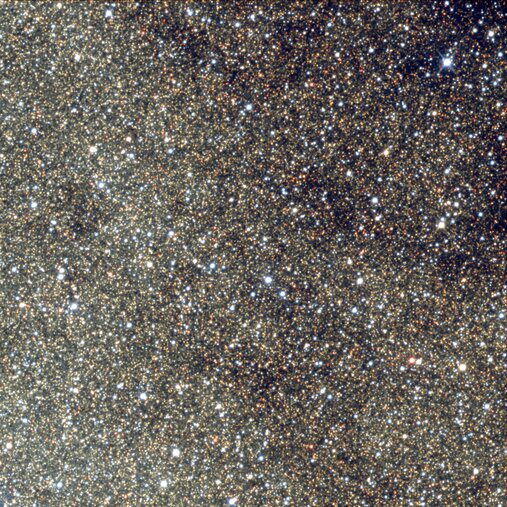
\includegraphics[width=0.5\linewidth]{../static/microlensing/crowded_field.jpg}
        \caption{
            Stellar field of a microlensing event GLE-2012-BLG-0406 (centered),
            imaged by one of Las Cumbres Observatory's 2m telescopes,
            showing the high density of stars typical in microlensing observations.
            Credit: Y. Tsapras. Taken from
            \url{http://microlensing-source.org/pictures/}.}
        \label{fig:crowded_field}
    \end{centering}
\end{figure}

That the same effect could be used to detect the presence of planets orbiting
around the lens star was first theorized by \citet{1964PhRv..133..835L} who
wrote that \emph{``the primary effect of planetary deflectors bound to stars
    other than the Sun will be to slightly perturb the lens action of these
    stars''} although he was also sceptical about the possibility of detection,
saying that \emph{``associated pulses would be so weak and infrequent and of
    such fleeting duration – perhaps a few hours – as to defy detection''}.
Gravitational lensing as a method for discovering exoplanets really took off
with the work of Paczy\'nski
\citep{1986ApJ...304....1P,1986ApJ...301..503P,1991ApJ...374L..37M} who also
coined the term \emph{microlensing}, which refers to gravitational lensing in a
regime where the images of the background object cannot be resolved but one can
nevertheless measure its magnification as a function of time. Microlensing as a
method for detecting exoplanets has some unique aspects. First, it is a one-off
event which happens on a timescale of a few minutes up to several months
depending on the distances to the background star and the lensing star and the
mass of the lens. In addition to the fact that there's only one chance to
observe such an event for it to happen at all requires extremely precise
alignment between the lens and the background star and the chance of observing
a stellar microlensing event is about one-in-a-million (CITE) for a typical
star within the Milky Way. To observe a planetary signal is about an order of
magnitude less likely than that. Hence, obtaining a decent sample of planetary
events requires continuous monitoring on the order of $10^{8}$ stars at the
time which way microlensing observations that to focus on the densest region of
the Milky Way -- the galactic bulge. Figure~\ref{fig:crowded_field} a picture
from of such a dense stellar field. Finally, in the vast majority of cases we
do not detect any light from the lens itself, the collected photons are from a
background star completely unrelated and distant from the lensing star. This is
very different from other exoplanet discovery methods and it means that we only
obtain dynamical properties of planets such their masses and periods.

The aspects that make microlensing events that make them difficult to observe
also mean that it provides a unique lens onto exoplanet systems. Relative to
other methods such as transits and radial velocity, microlensing is sensitive
to planets located at substantially greater distances, well outside of our
Solar System neighborhood and even potentially to Milky Way's satellite
galaxies such as the Magellanic Clouds and the nearby Andromeda galaxy (CITE).
Microlensing is also sensitive to very to very small planets and planets which
are further out from the star than those typically detected using transits and
radial velocity. Microlensing surveys such as OGLE \citep{1993AcA....43..289U}
and MOA \citep{1999PThPS.133..233M} have been continuously monitoring crowded
stellar fields in the Milky Way since the 90s\footnote{Initially the focus was
    on finding dark matter candidate particles -- so called MACHOs (Massive Compact
    Halo Objects).} discovering thousands of stellar events and dozens of planetary
events. In order to detect planetary deviations in the observed light curve it
essential to have high cadence observations of the source star. The way surveys
have traditionally worked is that once a particular star started to become
magnified many additional small telescopes would start observing it to obtain
denser coverage and sometimes space-based observatories get involved as well.
The vast majority of microlensing events analyzed so far consist of
observations from multiple observatories, each with its own unique aspects such
as noise properties, cadence and photometric quality.

Future surveys such as the ground based Rubin Observatory
\citep{2019ApJ...873..111I} telescope and the space based Roman Telescope
\citep{2019ApJS..241....3P} and Euclid \citep{2022arXiv220209475B} will detect
tens of thousands of events in total. Although most of past work in the field
focused on characterizing individual events binary lens events, answering
questions about \emph{populations} with these new (but also existing) datasets
requires scalable data analysis methods and algorithms and a clear set of
guidelines on how to interpret the analysis products. This is a substantial
challenge because microlensing events are notoriously difficult to model. Even
though the datasets are relatively simple, consisting of multiple time series
photometric light curves in different bands, the parameter space of even the
simplest models is highly non-linear, correlated, relatively high dimensional
and there are often near perfect degeneracies in the solutions.

The assumptions that existing methods for modeling microlensing events rely on
are often opaque and unquestioned. Discussions on model ``degeneracies''
\citep{2014MNRAS.437.4006S,2019AJ....157...23H,2018AcA....68...43S,2009MNRAS.393..816D},
correlated noise \citep{2015ApJ...812..136B,2019MNRAS.488.3308L} and model
comparison \citep{2018AJ....155..259H,2019MNRAS.484.5608D} have been ongoing in
the microlensing literature for decades without a clear solution and proper
framing of the issue. In this thesis I will revisit these kinds of questions
while taking into account many recent developments in the fields of
computational statistics and machine learning. My main contributions are the
following:
\begin{itemize}
    \item I wrote an open-source Python package \ssf{caustics} which enables fast and
          accurate computation of binary and triple lens microlensing light curves using
          contour integration. The code runs on both CPU and GPU architectures, and
          crucially, for reasons that I will elaborate in subsequent chapters, it
          supports \emph{automatic differentiation} of all outputs with respect to all
          input parameters which enables the use of statistical methods which are orders
          of magnitude more efficient than existing approaches. The code can easily be
          extended to support quadruple lensing and arbitrary intensity profiles for the
          source star.
    \item I have revisited the topic of degeneracies in the posterior probability
          distributions which appear in the context of microlensing and propose solutions
          to these problems.
    \item I have extended the complex polynomial root solver from \citet{Cameron2021}
          such that it can be executed on GPU architectures and that it supports
          automatic differentiation. This enables the evaluation of ~1M lens equation
          solutions for point source binary and triple lenses in seconds using a CPU and
          miliseconds using a GPU.
    \item I propose an approach to statistical inference on a population of microlensing
          events which different from existing methods and has some advantages.
    \item I briefly discuss the issue of correlated noise in microlensing light curves
          and propose ways to account for it using Gaussian processes.
\end{itemize}

\section{Occultation and phase curve mapping}
Interestingly, the second topic I will cover in this thesis has a history not
unlike that of microlensing. It was proposed in the early 20th century and it
was only much later that technology caught up with the idea. Back in 1906,
\citet{1906ApJ....24....1R} pointed out that certain features in light curves
of Solar System satellites may be attributed to inhomogeneities of their
surfaces. The key idea is that although at any given time we only observe the
total light from an unresolved satellite or planet, different portions of the
surface are visible at different times so we may expect that some of the
information about the surface intensity (be it emission from heat or reflected
Sunlight) gets imprinted onto the light curve. \citet{1906ApJ....24....1R} also
considered the inverse problem -- can we learn something about the surface of
these objects starting from a light curve? The method he proposed is now known
as \emph{phase curve mapping} and it was first attempted by
\citet{1972ApJ...174..449L} who analyzed photometric light curves of Pluto in
reflected light attempting to constrain variations in the \emph{albedo} of the
surface with inconclusive results.

Later works such as
\citet{1986AJ.....92.1201D,1992Icar...97..211B,1993Icar..102..134Y,1999AJ....117.1063Y}
went a step further by using not only phase curves but also light curves of
mutual \emph{occultations} of Pluto by its moon Charon to reconstruct albedo
maps with greater success. The major advantage of occultations relative to just
phase curves is that more information about the surface is encoded into the
light curve because of the sharp limb of the occultor sweeping over the disc of
an occulted body and blocking the reflected light. More importantly for this
thesis, \citet{1994Icar..107..195S} was the first to observe the occultations
of Jupiter's moon Io by another of Jupiter's moons -- Europa, and also
occultations of Io by Jupiter itself. These observations were conducted using
near-infrared telescopes such as NASA's Infrared Telescope Facility (IRTF) to
observe emitted light from Io's surface which is covered with many time-varying
and bright volcanic features. The observing campaign of Io has yielded insights
into the the nature of its volcanic activity and it continues to this day. I
will return to the subject of Io in great detail in
Chapter~\ref{ch:mapping_io}.

A natural question arises, can we do this with objects outside of the Solar
System? The answer is yes. \citet{2007Natur.447..183K},
\citet{2012ApJ...747L..20M}, and \citet{arXiv:1202.3829} used Spitzer
mid-infrared observations of secondary eclipses of the Hot Jupiter HD189733b
and found that surface emission is best described by the presence of a large
hot spot on the dayside of the planet which is longitudinally offset from the
substellar point. Similarly, \citet{2014Sci...346..838S}, produced temperature
maps of the Hot Jupiter WASP-43b, \citet{2013ApJ...776L..25D} mapped the Hot
Jupiter Kepler-7b in reflected light and \citet{2016Natur.532..207D} mapped the
thermal emission from the Super Earth 55 Cancri e. These studies were only able
to capture longitudinal variations in intensity. Real exoplanet atmospheres of
are certain to have three-dimensional spatial inhomogeneities in emission more
complex than a single hot spot due to the presence of clouds, zonal jets,
storms, waves etc. \citep{2020SSRv..216..139S}.

In recent years there have been significant advances in statistical modeling of
phase curves and eclipse light curves. Most notably,
\citet{2019AJ....157...64L} introduced the \ssf{starry} code which enables
analytic computation of phase curves and occultation light curves for bodies
with arbitrary emission maps expressed in a spherical harmonic basis (an idea
dating back to \citet{1906ApJ....24....1R} ) and \citet{2021arXiv210306275L}
expanded the algorithm for the (considerably more complicated) case of
reflected light. In this thesis, I will present the work I've done in
collaboration with other researchers from the planetary science and exoplanet
communities on using \ssf{starry} to map the surface of Io and investigate the
prospects for detecting fine spatial structure in the atmospheres of Hot
Jupiters using JWST phase curves and eclipse light curves. My contributions to
this area are the following:
\begin{itemize}
    \item I have developed a novel model for inferring emission maps of Io from
          occultation light curves. First part of this project is published in
          \citet{2022PSJ.....3...67B} though I haven't managed to complete the second
          part.
    \item I have investigated the problem of eclipse mapping of exoplanets using the
          \ssf{starry} framework, focusing in particular on the possibility of detecting
          planetary scale storms on Hot Jupiters using JWST. I found that it extremely
          difficult to infer maps of higher resolution than a dipole order but that
          should still be sufficient for detecting large scale weather and climate change
          in the atmospheres of these planets.
\end{itemize}
The application of the occultation/eclipse mapping method to Io can be seen as the
best case scenario for the application of the same method to exoplanets.
I will show that even in the case of observing a bright object right in our neighborhood,
this is by no means and easy task. Our ability to reconstruct the surface features of
Io sets a sort of upper limit on what is possible with exoplanets.

%\section{Outline}
%The outline of the thesis is as follows. Chapter~\ref{ch:theoretical_min}
%contains the theoretical background needed to understand the subsequent
%chapters, covering the theory behind microlensing and occultation mapping, a
%summary of Bayesian statistics in particular and statistical inference more
%generally, and probabilistic programming which ties everything together.
%Chapter~\ref{ch:microlensing_modeling} is the most extensive chapter in the thesis
%covering all of my work on microlensing. I start by discussing the case of
%single lens microlensing models, showing that it contains many of the
%properties of more complex models. In particular I focus on the issue of
%multi-modal posterior distributions which is a ubiquitous problem in
%microlensing. I propose several solutions to this and demonstrate their
%effectiveness. I then move on to the considerably more complex case of binary
%and triple lens models starting with numerical methods for solving the lens
%equation (finding roots of a complex polynomial equation). I demonstrate the
%advantage of the Ehrlich-Aberth algorithm over previous methods and explain how
%to make this algorithm differentiable and orders of magnitude faster through
%the use of GPUs. Next, I cover the contour integration algorithm for computing
%the magnification of a limb-darkened source star and its implementation in
%\ssf{caustics}.

% CHAPTER 2: The theoretical minimum
\chapter{The theoretical minimum}
\label{ch:theoretical_min}

\section{Gravitational microlensing}
\label{sec:microlensing}
Gravitational lensing is generally divided into multiple classes depending
on weather the effect is discernible at the level of individual objects or a
a statistical sample of object. The main division is between \emph{weak lensing}
and \emph{strong lensing}.
The former refers to lensing by galaxies and clusters of galaxies on cosmological
scales where the deflection  is impossible to detect in a single background source
but one can tease out the effect in a statistical sense.
Strong lensing refers to lensing of individual objects and it is further divided into
\emph{macrolensing} -- lensing of galaxies where the multiple images of the source
are resolved, and \emph{microlensing}  -- the images are generally not resolved,
and the observable is the total magnification of the source as a function of time (a light curve).
In case of microlensing the light source is either a quasar or a star (sometimes a binary star)
and the lenses are stars, brown dwarfs, planets, and compact objects such as black holes, neutron
stars and white dwarfs. In this thesis we focus specifically on microlensing
with stars as the light source instead of quasars\footnote{Quasar microlensing
    is a somewhat separate community from the rest of the microlensing community.}.

\subsection{Deflection of light by gravity}
Gravitational lensing is a phenomenon fully described by Einstein's General
Theory of Relativity (GR) in which light changes its direction of propagation
when passing close to a massive body. GR predicts the following:
\begin{itemize}
    \item the presences of mass changes the spacetime geometry from the flat (Minkowski)
          metric $\eta_{\mu\nu}$ to a curved metric, specified by the tensor $g_{\mu\nu}$
    \item massless particles such as photons follow the null geodesics -- minimum
          distance paths in curved spacetime which are obtained by solving the
          \emph{geodesic equation}
\end{itemize}
If we restrict ourselves to the regime where the metric is time independent
and the particles are allowed to travel at any velocity less than $c$,
also known as the \emph{weak field} or \emph{linearized approximation }
of GR, the metric tensor
can be written as
\begin{equation}
    g_{\mu\nu}=\eta_{\mu\nu}+h_{\mu\nu}\quad,
\end{equation}
where $h_{\mu\nu}=
    \textrm{diag}(-2\Phi,-2\Phi,-2\Phi,-2\Phi)$\footnote{Assuming the
    the metric sign convention $(-,+,+,+)$} \citep{carroll_2019}.
The (static) Newtonian gravitational potential $\Phi$ obeys the Poisson equation
\begin{equation}
    \nabla^2\Phi=4\pi G\rho\quad,
\end{equation}
where $\rho$ is the mass density of the distribution of mass located between the observer
and the light source.
The geometry of the lensing system consisting of a distant source of light, the
observer, and a distribution of mass with density $\rho$ located between the
source and the observer is shown in Figure~\ref{fig:deflection_angle}.
\begin{figure}
    \centering
    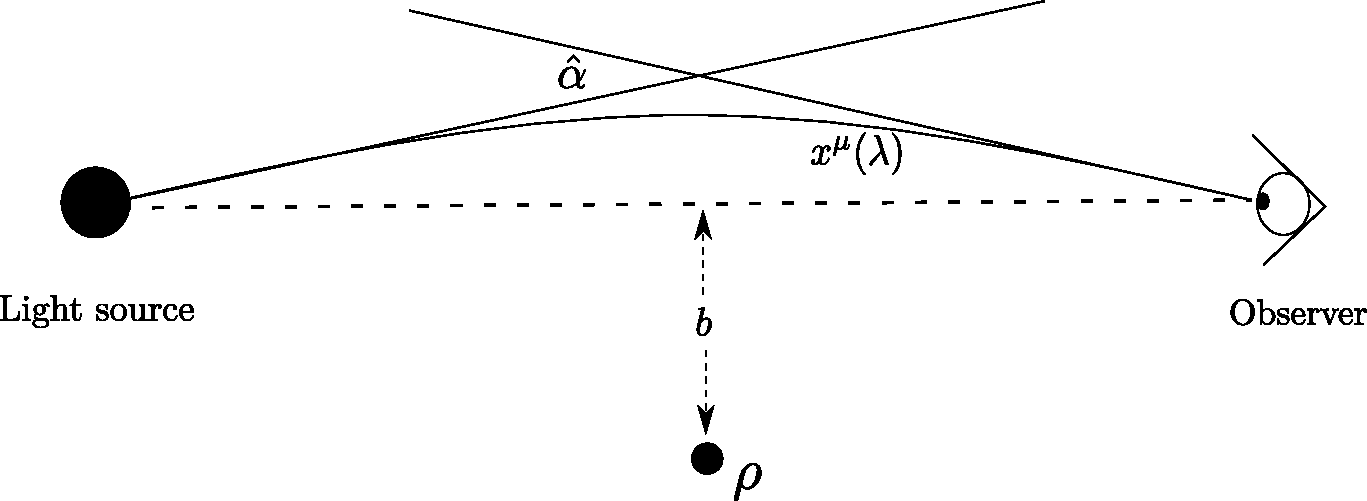
\includegraphics[width=0.6\linewidth]{../static/microlensing/deflection_angle.pdf}
    \caption{Geometry of gravitational lensing.
        A geodesic curve $x^\mu(\lambda)$ is deflected
        by an angle $\hat\alpha$ from its initial trajectory
        due to the presence of a massive body with mass density $\rho$. Figure
        adapted from \citet{carroll_2019}.}
    \label{fig:deflection_angle}
\end{figure}
A photon is deflected as it travels from a source to an observer by a
\emph{deflection angle} $\hat\alpha$, a vector in the
plane  perpendicular to the wave vector $\vec{k}$ pointing in the direction of
photon propagation.
The deflection angle is given by \citep{carroll_2019}
\begin{equation}
    \hat\alpha=2\int\nabla_\perp\Phi \ud s\quad,
    \label{eq:deflection_angle_general}
\end{equation}
where $\nabla_\perp\Phi$ is the gradient of the potential in the direction transverse
to the path of the photon and $s$ is the spatial distance traveled.
For a point mass $M$, the potential is given by the potential is
\begin{equation}
    \Phi=- \frac{GM}{(b^2+x^2)^{1/2}}\quad,
\end{equation}
where $x$ parametrizes the straight line distance between the observer and the lens and
$b$ is the impact parameter of the light ray.
Integrating from $-\infty$ to $\infty$ (i.e. assuming that both
the source and the observer are located far away from the deflecting mass), we obtain
the deflection angle:
\begin{equation}
    \hat\alpha= \frac{4GM}{c^2b}= \frac{2R_s}{b}\quad,
\end{equation}
where $R_s=2GM/c^2$ is the Schwarzschild radius.
$\hat\alpha$ is directly proportional to the mass of the lens and
it does not depend on the wavelength of the light. It also increases with the proximity of
the light ray to the lensing mass which is the opposite behavior to that of a
classical convex lens for which the deflection angle vanishes at the center of the lens.
The gravitational lens does not have a focal length and so it is not a lens in the usual
sense.
The resulting deflection angle is very small, for example, for the Sun we have
$GM/c^2=1.48\times 10^5\si{\centi\meter}$ (2.95 km), $R=6.96\times
    10^{10}\si{\centi\meter}$ and $\hat\alpha=1.75$ arc seconds. This is the angle
that was claimed to have been observed by Eddington when during the 1919 total
solar eclipse.

Equation~\ref{eq:deflection_angle_general} is only valid when the linearized
approximation of GR is sufficient. In this approximation, the deflection angles
are additive and the total deflection caused by a group massive bodies is just
the sum of the individual deflection angles. The linearized approximation
breaks down when the impact parameter $b$ approaches the Schwarzschild radius
of the lensing mass and the linearized metric is no longer sufficient. Except
for modeling lensing in the close vicinity of a black, the linearized
approximation is sufficient.

\subsection{The magnification of a point source by a point lens}
Consider a system consisting of an observer $O$, a point mass $M$, and a point
light source $S$. The geometry of this system is shown in
Figure~\ref{fig:lens_geometry}. The lens is located in the \emph{lens plane}, a
plane perpendicular to the observer--lens axis, at a distance $D_L$ away from
the source. The light source is located in the \emph{source plane}
perpendicular to the observer--source axis, at a distance $D_S$ away from the
observer, and the observer is in the \emph{observer plane}. The assumption that
the location of the source, observer, and the lens can be parametrized using
angular coordinates (or Cartesian coordinates if the distances to the lens and
the source are known) in their respective planes is justifiable because the
deflection angles involved are very small and the distance between the observer
and any point of interest in the lens plane is approximately constant.
\begin{figure}[!ht]
    \centering
    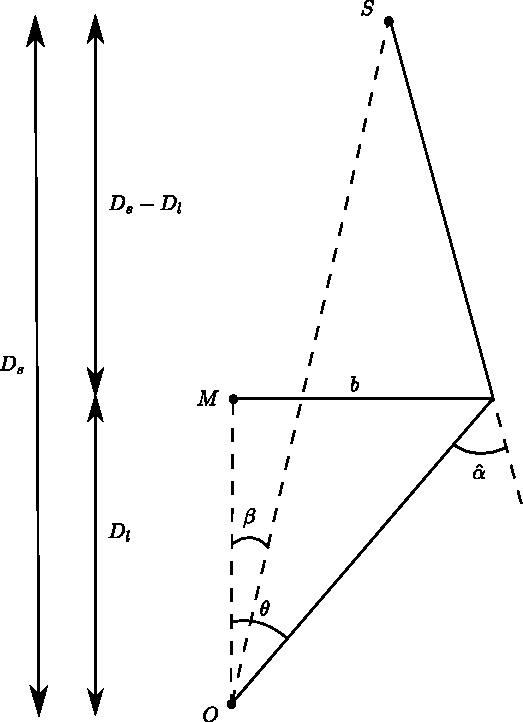
\includegraphics[width=0.4\linewidth]{../static/microlensing/lens_geometry.pdf}
    \caption{The geometry of a system consisting of a point mass lens $M$ located at distance
        $D_L$ at angular separation $\beta$ from the observer, and a single light source $S$ located at distance $D_S$, emitting a light ray which gets
        deflected by an angle $\hat\alpha$ from its
        original trajectory. As a result the observer sees the source at angular separation
        $\theta$. Figure adapted from \citet{1992grle.book.....S}.}

    \label{fig:lens_geometry}
\end{figure}
Let $\theta$ be the apparent angular position of the source in the sky with respect to the
observer--lens axis and $\beta$ be the actual angular position of the source.
Assuming a metric for spacetime in between the source and the observer that is
approximately Euclidian\footnote{This is a valid assumption for galactic sources but not for
    extragalactric source such as quasars and galaxies which require a cosmological
    model for the metric.} the distance from the lens to the
source is $D_S-D_L$.

From Figure~\ref{fig:lens_geometry} it follows that the relationship between
the observed and the actual location of the source is given by
\begin{equation}
    \beta=\theta-2 R_s \frac{D_S-D_L}{D_LD_S}
    \frac{1}{\theta}\quad,
    \label{eq:lens_equation}
\end{equation}
which is known as the \emph{lens equation} or sometimes also the \emph{ray-tracing}
equation. If the source and the lens are perfectly aligned with respect to the observer,
then $\beta=0$ and $\theta\equiv\theta_E$ where
\begin{equation}
    \theta_E= \sqrt{ \frac{4GM}{c^2} \left( \frac{1}{D_L} - \frac{1}{D_S} \right)}=
    \sqrt{\kappa M\pi_{LS}}
    \label{eq:angular_einstein_radius}
\end{equation}
where $\kappa \equiv \frac{4 G}{c^{2} \mathrm{au}} \simeq 8.1 \frac{\mathrm{mas}}{M_{\odot}}$
and
\begin{equation}
    \pi_{LS}\equiv\pi_L - \pi_S=\frac{1\mathrm{au}}{D_L}-\frac{1\mathrm{au}}{D_S}
\end{equation}
is the relative lens-source parallax.

The image of the source forms a ring (the Einstein ring) around the lens star
with angular radius $\theta_E$ -- the \emph{Einstein radius}. $\theta_E$
depends on the mass of the lens and the distances to the lens and the source.
The angular Einstein radius sets the characteristic scale of a microlensing
event, it is a natural unit for most microlensing parameters. For an M-dwarf
star lens in the galactic disc ($D_L\sim 3\,\textrm{kpc}$) and a source star in
the galactic bulge ($D_S\sim 8\,\textrm{kpc}$) we have $\theta_E\sim
    1\,\textrm{mas}$ so the typical scale of microlensing is on the order of
miliarcseconds. The images of the source star are only rarely observable using
the most advanced optical interferometers such as the GRAVITY instrument on
ESO's Very Large Telescope whose lower resolution limit is $2\,\textrm{mas}$
\citep{arXiv:1705.02345}. \cite{2019ApJ...871...70D} were the first to resolve
the images of a microlensing event, finding the value of
$\theta_E=1.87\,\textrm{mas}$ using the GRAVITY instrument.

We can rewrite Equation~\ref{eq:lens_equation} by defining new dimensionless
angular coordinates scaled by the angular Einstein radius:
\begin{equation}
    z\equiv \frac{\theta}{D_L\theta_E}, \quad w\equiv\frac{\beta}{D_S\theta_E}
\end{equation}
The lens equation then takes the very simple form
\begin{equation}
    z= w- \frac{ 1}{w}
    \label{eq:lens_equation_dimensionless}
\end{equation}
Equation~\ref{eq:lens_equation_dimensionless} is a nonlinear mapping between the
source plane $w$ and the image plane $z$.
If we solve for $z$, we obtain two solutions for the position of the images, given by

\begin{equation}
    z_\pm= \frac{1}{2} \left( w\pm\sqrt{w^2 +4}\right)
    \label{eq:images_location}
\end{equation}
For non zero $w$ the so called \emph{minor image} is always located
within the Einstein radius ($\lvert z_-\rvert<1$) while the \emph{major image}
is located outside of it ($\lvert z_+\rvert>1$).

Since gravitational lensing does not involve any additional emission or
absorption along a deflected ray of light and since the wavelength of the light
ray does not change when it encounters the lens, the \emph{surface brightness}
(flux density per unit angular area) $I$ of the source image is identical to
the surface brightness of the unlensed source. The flux of an infinitesimal
source is a product of the surface brightness and the solid angle $\Delta
    \omega$ subtended by the source in the sky which changes throughout the
microlensing event because the source and the lens are in motion relative to an
observer. The ratio of the original and the lensed source flux, the
\emph{magnification} $A$, is then given by the ratio of the two solid angles
\begin{equation}
    A= \frac{\Delta \omega}{(\Delta\omega)_0}\quad,
    \label{eq:magnification}
\end{equation}
where $0$ denotes the unlensed solid angle.
Assuming an infinitesimal source size at angular location
$\mathbf w \equiv (w_1,w_2)$ subtending an angle
$\Delta (\omega)_0$, and an image of the source at location
$\mathbf z\equiv(z_1,z_2)$ subtending an angle
$\Delta \omega$; the ratio between the solid angle of the source and the image
is given by the determinant of the Jacobian matrix of the
lens mapping $\mathbf{z}\rightarrow\mathbf{w}$, evaluated at the location of
the images
\begin{equation}
    \frac{(\Delta\omega)_0}{\Delta\omega} =\left\lvert\textrm{det}
    \frac{\partial \mathbf w}{\partial \mathbf z} \right\rvert
\end{equation}
The magnification $A$ is then given by the inverse Jacobian determinant
of the lens mapping:
\begin{equation}
    A= \left\lvert\det
    \frac{\partial \mathbf w}{\partial \mathbf z} \right\rvert^{-1} \label{eq:magnification_general}
\end{equation}
The images for which the determinant of the Jacobian of the lens mapping is
positive are said to have positive \emph{parity} and vice versa.

Looking at Equation~\ref{eq:magnification_general}, we see that the
magnification diverges when the Jacobian determinant of the lens mapping
vanishes. Curves in the lens plane for which the determinant of the lens
mapping vanishes, that is,
\begin{equation}
    \left\lvert\det
    \frac{\partial \mathbf w}{\partial \mathbf z} \right\rvert=0
\end{equation}
are called \emph{critical curves}.
The critical curves in the lens plane can be mapped to the source plane using
the lens equation $\mathbf{z}\rightarrow \mathbf{w}$ and these curves are
are called \emph{caustic curves}.
Although the magnification factor in Equation~\ref{eq:magnification_general} formally
diverges at the points of critical curves or caustics,
the divergence is not physical because light sources aren't truly point like.
If the finite angular size of the source is taken into
account, the magnification is an integral of Equation~\ref{eq:magnification_general} over the
extent of the source, weighted by the source brightness and that integral is always finite.
Both the critical and the caustic curves are closed and one can prove that \textbf{the
    number of images changes by two if and only if the source crosses a caustic curve}
\citep[][Chapter 6]{1992grle.book.....S}.

We can derive a simpler expression for Equation~\ref{eq:magnification} by
switching to polar coordinates $(v,\phi)$ in the lens plane. The lens equation
for the two vector components of the apparent source position is given by
\begin{align}
    w_1= & z_1- \frac{z_1}{z_1^2+z_2^2} \\
    w_2= & z_2- \frac{z_2}{z_1^2+z_2^2}
\end{align}
Introducing polar coordinates $z_1=v\cos\phi,\;z_2=v\sin\phi$, we have
\begin{equation}
    \left\lvert\textrm{det}
    \frac{\partial \mathbf w}{\partial \mathbf z} \right\rvert =1- \frac{1}{v^4}\quad,
\end{equation}
By substituting in the locations of the source images
Equation~\ref{eq:images_location} into the
above expression, we obtain the magnification of the source for both images
\begin{equation}
    A_\pm = \frac{1}{2}\left(\frac{u^{2}+2}{u \sqrt{u^{2}+4}} \pm 1\right)
    \label{eq:magnification_per_image}
\end{equation}
where $u = \sqrt{w_1^2+w_2^2}$ is the the magnitude of the position
vector of the source star.
The total magnification is then the sum of the two magnifications, and is given by
\citep{1936Sci....84..506E}
\begin{equation}
    A(u)=\lvert A_-\rvert+\lvert A_+\rvert= \frac{u^2+2}{u\sqrt{u^2+4}}\quad,
    \label{eq:magnification_point_lens}
\end{equation}
The critical curve of the point lens is the Einstein
ring corresponding to $v=\sqrt{z_1^2+z_2^2}=1$ and the caustic curve is mapped to a
a single point in the source plane at $u=0$.
For source separations much smaller than the angular Einstein radius ($u\ll 1$), the
magnification is approximately $A(u)\simeq 1/u$, in the opposite case ($u\gg 1$)
we have $A(u)\simeq 1+ 2/u^4$, that is, the magnification falls off rapidly the further
away the source is from the lens.

To be able to evaluate Equation~\ref{eq:magnification_point_lens} in practice
we have to parametrize the position of the source on the sky $u$ as a function
of time. To derive an expression for $u(t)$ we assume the the motion of the
observer, lens and the source is rectilinear (acceleration can be neglected).
We take $\vec{w}_S$ to be the angular position of the source star on the plane
of the sky and $\boldsymbol{\mu}_L$ to be its proper motion vector. Likewise
for the lens. We thus have
\begin{align}
    \vec{w}_S(t) & =\vec{w}_{S, 0}+
    \left(t-t_{0}\right) \boldsymbol{\mu}_S
    \label{eq:source_position}      \\
    \vec{w}_L(t) & =\vec{w}_{L, 0}
    +\left(t-t_{0}\right) \boldsymbol{\mu}_L\quad,
    \label{eq:lens_position}
\end{align}
where $t_0$ is some reference time.
The relative position vector of the lens with respect to the source is then
\begin{equation}
    \boldsymbol{u}(t) \equiv \frac{\vec{w}_L(t)
        -\vec{w}_S(t)}{\theta_E}=
    \frac{\vec{w}_{LS, 0}}{\theta_E}
    +\frac{t-t_{0}}{\theta_E} \boldsymbol{\mu}_{LS}
    \label{eq:relative_trajectory_no_parallax}
\end{equation}
where
$\vec{w}_{L S, 0}\equiv\vec{w}_{L,0}-\vec{w}_{S, 0}$
is the relative position at $t_0$ and
$\boldsymbol{\mu}_{LS}\equiv \boldsymbol{\mu}_{L}- \boldsymbol{\mu}_{S}$ is the
relative proper motion.
Since $\boldsymbol{\mu}_{LS}$ and $\vec{w}_{L S, 0}$ are
perpendicular to each other, it follows that the magnitude of the relative
separation is
\begin{equation}
    u(t)=\sqrt{u_0^2+ \left(\frac{t-t_0}{t_E}\right)^2}
\end{equation}
where we have defined $u_0\equiv |\vec{w}_{L S, 0}|/\theta_E$
and $t_E\equiv \theta_E/|\boldsymbol{\mu}_{LS}|$.
The magnification is a function of three parameters $(t_0, u_0, t_E)$
and the resulting curve as a function of time is often called the Paczy\'nski curve
\citep{1986ApJ...304....1P,1986ApJ...301..503P}.
The magnification as a function of time for different impact parameters $u_0$
is shown in Figure~\ref{fig:paczynski_curve}. Notice the very steep fall off in
magnification as as we move away from the Einstein ring ($A(u)\propto
    1+2u^{-4}$).
In the limits of $u_0\rightarrow 0$ and $u_0\gg 1$  there is a continuous
mathematical degeneracy between the parameters $t_0$, $u_0$ and $t_E$
\citep{1997ApJ...487...55W}.

\begin{figure}[t]
    \begin{centering}
        \includegraphics[width=0.7\linewidth]{figures/paczynski_curve.pdf}
        \caption{
            Magnification of a point source by a point lens as a function of time. The
            various magnification curves correspond to different impact parameters $u_0$.
            The inset figure
            shows the source trajectories in the lens plane, the dashed circle corresponds
            to the Einstein radius $v=1$.}
        \label{fig:paczynski_curve}
        \script{paczynski_curve.py}
    \end{centering}
\end{figure}

\subsection{Observed flux}
The magnification $A(t)$ is not a direct observable in microlensing events. We
can only measure the flux of the source star which is usually contaminated with
the flux of other nearby stars in the dense stellar field and potentially also
with light from the lens and possible companions to the lens. The observed flux
is thus given by
\begin{equation}
    F(t)=F_S\,A(t)+F_B
    \label{eq:flux_observed_micro}
\end{equation}
where $F_s$ is the flux of the source star and $F_B$ is the contamination flux also
called the \emph{blending flux}. To quantify the strength of the blending e can
define the emph{source flux fraction} $b_S$ as the fraction of total (unmagnified)
flux that is coming from the source star:
\begin{equation}
    b_S\equiv F_S/(F_S + F_B)
\end{equation}
For highly blended events $b_S\approx 0$ and in absence of blending $b_S=1$.
The source flux $F_S$ and the blending flux $F_B$ are generally highly correlated
and it is often preferable to use a slightly different parametrization proposed by
\citet{2009MNRAS.393..816D}. In this parametrization we use the
\emph{baseline flux} $F_\mathrm{base}$ and the difference between
the baseline flux and the flux at peak magnification $\Delta F\equiv F_S[A(u_0)-1]$
as the new parameters.
Equation~\ref{eq:flux_observed_micro} then takes the form
\begin{equation}
    f=\Delta F\frac{A(t) - 1}{A(t_0)-1}+F_\mathrm{base}
    \label{eq:flux_dominik}
\end{equation}
It is generally straightforward to measure the flux difference $\Delta F$, the
baseline flux $F_\mathrm{base}$ and the center of the curve $t_0$ but getting a
good estimate of $t_E$ even outside of the regime $u_0\rightarrow 0$ and
$u_0\gg 1$ requires good photometric sampling along the ``wings'' of the light
curve \citep{2009MNRAS.393..816D}.

\subsection{Astrometric microlensing}
\label{ssec:astrometric_microlensing}
\begin{figure}[t]
    \begin{centering}
        \includegraphics[width=0.7\linewidth]{figures/single_lens_astrometric_shift.pdf}
        \caption{
            Astrometric shift in the centroid of light for a point source point lens
            model.
            The various curves correspond to different impact parameters $u_0$.}
        \label{fig:single_lens_astrometric_shift}
        \script{single_lens_astrometric_shift.py}
    \end{centering}
\end{figure}

In addition to the photometric microlensing effect, there is the astrometric
effect -- the relative shift in the \emph{position} of the source star as the
star is being magnified. In case of a point source and a single lens we can
obtain the centroid of the two images by weighing their positions
(Equation~\ref{eq:images_location}) with their magnifications
(Equation~\ref{eq:magnification_per_image}):
\begin{equation}
    \vec w_c=\frac{A_+\vec w_+ + A_-\vec w_-}{A_+ + A_-}
\end{equation}
where $\vec w_c$ is the position of the centroid. It follows that the magnitude of the
shift is
\begin{equation}
    w_c=\frac{1}{2}\left(\frac{u(u^2 + 4)}{u^2+2}+u\right)
\end{equation}
and the magnitude $\delta w_c$ of the shift
$\delta \vec w_c\equiv\vec w_c - \vec u$ relative to the source star is
\begin{equation}
    \delta w_c = \frac{u}{u^2 + 2}
\end{equation}
The centroidal shift is plotted in Figure~\ref{fig:single_lens_astrometric_shift} for
different values of the impact parameter $u_0$. The trajectories trace out ellipses
\citep{1995ApJ...453...37W}.
Whereas the photometric effect is
strongest for
$u\ll 1$  the astrometric shift peaks at $u=\sqrt{2}$ with
$\delta w_{c,\max}\approx 0.354$ in units of the angular Einstein radius.
Importantly, the astrometric shift falls of as $1/u$ for $u\gg \sqrt{2}$  which is
much slower than $A\propto 1/u^4$ for the photometric effect.

\subsection{Magnification of an extended source}
\begin{figure}[t]
    \begin{centering}
        \includegraphics[width=\linewidth]{figures/single_lens_images.pdf}
        \caption{Images of an extended limb-darkened source star lensed by a single
            point lens for varying position of the source star. The top panels show the magnification map with a logarithmic scale
            colormap  consisting of a single point caustic. The semi-transparent circle
            is the source star disc with radius $\rho_\star=0.15$. The bottom row shows
            the two images merging into the Einstein ring as the source moves over the caustic.}
        \label{fig:single_lens_images}
        \script{single_lens_images.py}
    \end{centering}
\end{figure}
For a relatively small subset of microlensing events the source star passes
very close to the caustic and the variation of magnification over the extent of
the source star disc is non-negligible. For those events the point source
approximation breaks down and we have to take into account the finite angular
radius $\theta_\star$. This will generally happen when $u_0 \lesssim
    \rho_\star/2$ \citep{1997ApJ...477..580G} where
$\rho_\star=\theta_\star/\theta_E$. The effect of finite source effects on the
magnification curve thus matters only near the peak of an event and it results
in a rounder top of the curves shown in Figure~\ref{fig:paczynski_curve}.
Unfortunately there are no analytic solutions for the magnification of an
extended source lensed by a single point lens with a general surface brightness
profile. \citet{1994ApJ...421L..71G} derived an approximate solution valid for
uniform brightness sources with $\rho_\star\lesssim 0.1$ and
\citet{1994ApJ...430..505W} derived a general solution (also for a uniform
brightness source) involving solutions to elliptic integrals of the first,
second and third kinds. \citet{2009ApJ...695..200L} proposed a simple method for
numerically integrating the point source magnification over the extent of the source
disc which is fast and accurate for arbitrary intensity profiles.
Another solution involving Fast Fourier Transforms any source profile was
recently proposed by \citet{2022arXiv220306637S}.

In Figure~\ref{fig:single_lens_images} we show the magnification map and the
images of an extended limb-darkened source with $\rho_\star=0.15$ as it
approaches the point caustic for a single lens. The top panels show the
magnification map in the source plane using a logarithmic scale colormap. The
source disc is shown (semi-transparent grey circle) at different positions
relative to the caustic. The bottom panels show the resulting images in the
image plane, this is what we would see on the sky if we could resolve the
microlensing event. As the source moves closer to the caustic the area (and
hence the magnification) of the two images increases and eventually they merge
forming an Einstein ring.

To produce these plots I evaluated the lens mapping
(Eq.~\ref{eq:lens_equation_dimensionless}) on a regular grid in the image plane
and then plotted the surface brightness of the corresponding point on the
source disc in the source plane. I will discuss all of this in far greater
detail In Chapter~\ref{ch:microlensing_modeling} but for now I should mention a
few key points:
\begin{itemize}
    \item Every point inside the two images maps to a single point on the source disc via
          the lens equation. The inverse mapping is one-to-many because each point on the
          source disc maps to two points (point lens images) in the image plane. The
          points on the limbs of the two images correspond to the points on the limb of
          the source disc. We cannot predict the location of the images without inverting
          the lens mapping
    \item To numerically compute the magnification of an extended source, we could either
          integrate the magnification function convolved with the source brightness
          profile over the entire source disc (a two-dimensional integral), or we could
          do the same integral in the image plane. The first approach is highly
          numerically unstable because we would need to integrate over a function which
          diverges as $1/r$ approaching the caustic and this would require a very large
          number of lens equation evaluations. Hence it is much better to integrate in
          the image plane where the function is smooth.
    \item Decreasing the source radius $\rho_\star$ results in narrower arcs of the
          images (smaller radial extent).
\end{itemize}

\subsection{Annual parallax}
\label{ssec:single_lens_parallax}
In Equation~\ref{eq:relative_trajectory_no_parallax} we have assumed that the
relative motion of the lens with respect to the source on the plane of the sky
is rectilinear.
This is a reasonable approximation in a barycentric frame of
reference if the acceleration of the source and the lens can be neglected.
However, most microlensing events are observed from a non-inertial geocentric
frame (Earth) and sometimes also from multiple locations simultaneously. In those
cases we have to take into account parallax effects.
We differentiate between two kinds of parallax. First is the \emph{annual
    parallax} (sometimes also called the orbital parallax) which modifies the
lens-source relative motion vector $\boldsymbol\mu_{LS}$ due to the local
acceleration of Earth in its orbit. It is important for long timescale events
when the event timescale is equal to some substantial fraction of a year. The
effect of annual parallax is usually a slight modification of the shape of the
Paczy\'nski curve.

The second kind of parallax is the \emph{satellite parallax} which refers to a
difference in viewpoint when conducting simultaneous observations of the source
star from different locations separated by a substantial fraction of the
Einstein ring projected onto the observer plane $\tilde{r}_E\equiv
    D_{LS}\theta_E$ (where $D_{LS}^{-1}=D_L^{-1} - D_S^{-1}$). In practice this
means observing a microlensing event from Earth and a space based telescope
simultaneously. It was first proposed by \citet{1966MNRAS.134..315R}. There is
also the ``terrestrial parallax'' which is identical to the satellite parallax
except that it involves only ground-based observations separated by a large
fraction of Earth's diameter. A measurement of these parallax effects allows
for a partial breaking of the degeneracy in the event timescale $t_E$ by
providing a relationship between the mass and the distance to the lens
(assuming one can estimate the distance to the source star).

In this section I will describe the annual parallax effect. We start by
modifying Equations~\ref{eq:source_position} and \ref{eq:lens_position} to
include the projected motion of the Sun relative to the Earth on the plane of
the sky. We project $\mathbf s$ -- the position vector of the Sun relative to
Earth, onto a plane perpendicular to the line of sight towards the source star
(plane of the sky) which is defined by the unit vector $\boldsymbol{\hat n}$
normal to the plane. The unit vector $\boldsymbol{\hat n}$ depends on the sky
coordinates of the source star $(\alpha,\delta)$ (right ascension and
declination). We choose to work in geocentric equatorial coordinates defined by
the spherical unit vectors $\hat{\mathbf e}_n$, pointing North, and
$\hat{\mathbf e}_e$ pointing eastward such that the coordinate system is
right-handed. The unit vectors are defined by
\begin{align}
    \hat{\mathbf e}_e & = \hat{\mathbf z}\times \hat{\mathbf n}  \\
    \hat{\mathbf e}_n & = \hat{\mathbf n}\times\hat{\mathbf e}_e
\end{align}
The two components of $\mathbf s$ projected onto the plane of the sky are then
\begin{align}
    \zeta_e(t;\alpha,\delta)\equiv \mathbf s\cdot \hat{\mathbf e}_e \\
    \zeta_n(t;\alpha,\delta)\equiv \mathbf s\cdot \hat{\mathbf e}_n
\end{align}
In practice, we can retrieve $\mathbf{s}$ using NASA's JPL Horizons system and compute
the projected separation at any time $t$.
The angular positions of the source and the lens
(Equations~\ref{eq:source_position} and \ref{eq:lens_position}) then become
\begin{align}
    \vec{w}_S(t) & = \vec{w}_{S,0}+(t-t_0)\boldsymbol{\mu}_S
    +\pi_S\,\boldsymbol{\zeta}(t)                            \\
    \vec{w}_L(t) & = \vec{w}_{L,0}+(t-t_0)\boldsymbol{\mu}_L
    +\pi_L\,\boldsymbol{\zeta}(t)
\end{align}
where  $\pi_S\equiv 1\,\mathrm{au}/D_S$ is the source parallax, and $\pi_L$ is the
lens parallax.
The relative separation is then
\begin{equation}
    \boldsymbol{u}(t)= \frac{\boldsymbol\theta_{LS, 0}}{\theta_E}
    +\frac{t-t_0}{\theta_E}\boldsymbol{\mu}_{LS}+\pi_{E}\,\boldsymbol{\zeta}(t)
    \label{eq:relative_separation_parallax}
\end{equation}
where
\begin{equation}
    \pi_E\equiv \frac{\pi_{LS}}{\theta_E}
    \label{eq:pi_E}
\end{equation}

Since annual parallax is a higher order effect affecting the apparent
trajectory of the source on the sky, it makes sense to decompose the trajectory
as a sum of rectilinear motion plus a deviation due to parallax. Following
\citet{2004ApJ...606..319G} we define the position offset of the Sun on the
plane of the sky relative to its position at a particular time $t_0'$ as

\begin{equation}
    \delta\boldsymbol \zeta (t)=\boldsymbol \zeta (t)-\boldsymbol \zeta (t_0')-(t-t_0')
    \boldsymbol{\dot \zeta} (t_0')
\end{equation}
By construction, we have $\delta\boldsymbol \zeta (t_0')=0$ and
$\delta\dot{\boldsymbol \zeta} (t_0')=0$.
Equation~\ref{eq:relative_separation_parallax} then takes the form
\begin{equation}
    \boldsymbol{u}(t)=\mathbf{u}_0 + (t-t_0')\,\dot{\mathbf{u}}_0 +
    \pi_E\,\delta\boldsymbol \zeta(t)
    \label{eq:relative_separation_parallax_decomposed}
\end{equation}
where
\begin{align}
    \mathbf{u}_0       & \equiv \mathbf{u}(t_0) =\frac{\boldsymbol\theta_{LS, 0}}{\theta_E}
    + \frac{(t_0'-t_0)}{\theta_E}\boldsymbol\mu_{LS}+
    \pi_E\,\boldsymbol \zeta(t_0)                                                           \\
    \dot{\mathbf{u}}_0 & \equiv\dot{\mathbf{u}}(t_0)=
    \frac{\boldsymbol\mu_{LS}}{\theta_E}  + \pi_E\,\dot{\boldsymbol \zeta}
    (t_0')
\end{align}
In what follows, we set the reference time to $t_0'\equiv t_0$ in order to ensure that
the vectors $\mathbf{u}_0$ and $\dot{\mathbf{u}}_0$ are perpendicular to each other,
which is the case at $t=t_0$ because at $t_0$ the trajectory has a local extremum
\footnote{In CITE, $t_0'$ is fixed to a particular value. It is not clear
    to me how this ensures that the two vectors are perpendicular to each other
    (TODO: show that this is true).}

\subsubsection{$\mathbf{u}(t)$ in the $(\mathbf{\hat e}_\bot,
        \mathbf{\hat e}_\parallel)$ coordinate system}%

\begin{figure}
    \centering
    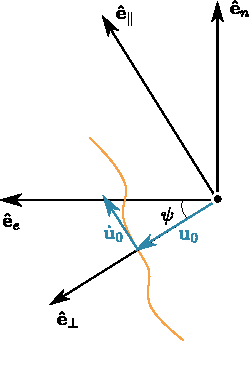
\includegraphics[width=0.3\linewidth]{../static/microlensing/microlensing_parallax_coordinates.pdf}
    \caption{A coordinate system
        $(\mathbf{\hat e}_\bot,\mathbf{\hat e}_\parallel)$ parallel to the source trajectory at time $t_0$. The orange curve
        represents the source trajectory relative to the lens at the origin. The
        coordinate system $(\mathbf{\hat e}_\bot,\mathbf{\hat e}_\parallel)$ is related to the equatorial coordinates $(\mathbf{\hat
                e}_e,\mathbf{\hat e}_n)$ by a rotation through an angle $\psi$.}
    \label{fig:parallax2}
\end{figure}

To evaluate Equation~\ref{eq:relative_separation_parallax_decomposed}, we need
to choose a suitable basis. A natural coordinate system for describing the
trajectory of the source relative to the lens is one defined by unit vectors
$(\mathbf{\hat e}_\bot,\mathbf{\hat e}_\parallel)$ where $\mathbf{\hat e}_\parallel$ is parallel to the trajectory $\mathbf{u}(t)$ at time $t_0$
(Figure~\ref{fig:parallax2}). We define the unit vectors as
\begin{equation}
    \mathbf{\hat e}_\bot\equiv \frac{\mathbf{u}_0}{|\mathbf{u}_0|}\quad,
    \mathbf{\hat e}_\parallel\equiv \frac{\mathbf{\hat n}\times\mathbf{u}_0}{|\mathbf{u}_0|}\quad
\end{equation}
and the coordinate system $(\mathbf{\hat e}_\bot,\mathbf{\hat e}_\parallel)$ is related to ecliptic coordinates via a simple rotation through an
angle $\psi$
\begin{equation}
    \begin{pmatrix}
        \mathbf{\hat e}_\bot \\
        \mathbf{\hat e}_\parallel
    \end{pmatrix}
    =
    \begin{pmatrix}
        \cos\psi & -\sin\psi \\
        \sin\psi & \cos\psi
    \end{pmatrix}
    \begin{pmatrix}
        \mathbf{\hat e}_e \\
        \mathbf{\hat e}_n
    \end{pmatrix}
    \label{eq:ecliptic_to_parallel}
\end{equation}
By construction, at time $t_0$ we have
$\mathbf{u}_0\,\bot\,\dot{\mathbf{u}}_0$ and the two components of
$\mathbf{u}(t)$ are then
\begin{align}
    u_\bot(t)      & \equiv \mathbf{u}(t)\cdot \mathbf{\hat e}_\bot= u_0 +
    \pi_E\,\delta\boldsymbol \zeta(t)\cdot\mathbf{\hat e}_\bot                                                                                                                                       \\
    u_\parallel(t) & \equiv \mathbf{u}(t)\cdot \mathbf{\hat e}_\parallel= (t-t_0)\,\dot{\mathbf{u}}_0\cdot\mathbf{\hat e}_\parallel+ \pi_E\,\delta\boldsymbol \zeta(t)\cdot\mathbf{\hat e}_\parallel
\end{align}
using the definitions of the unit vectors and
$\delta\boldsymbol \zeta(t)=
    \delta \zeta_e(t)\,\mathbf{\hat e}_e+\delta \zeta_n(t)\,\mathbf{\hat e}_n$, we have
\begin{align}
    u_\bot(t)      & = u_0 + \pi_E\,\cos\psi\,\delta \zeta_e(t) - \pi_E\,\sin\psi\,\delta \zeta_n(t)
    \label{eq:u_t_parallel1}                                                                         \\
    u_\parallel(t) & =(t-t_0)/t_E' + \pi_E\,\sin\psi\,\delta \zeta_e(t) +
    \pi_E\,\cos\psi\,\delta \zeta_n(t) \label{eq:u_t_parallel2}
\end{align}
where $t_E' =|\dot{\mathbf{u}}_0|=|\boldsymbol\mu_{LS}/\theta_E  + \pi_E\,\dot{\boldsymbol \zeta}(t_0')|$.
The model parameters which determine the magnification $A(t)$ are then
$\left(u_0,t_0,t'_E,\pi_E,\psi\right)$. Notice that $u_0$ in this case can also be negative.

An alternative parametrization which is more commonly used is obtained by
defining components of a "microlensing parallax vector" as
\begin{align}
    \pi_{E,N} & \equiv \pi_E\cos\psi \\
    \pi_{E,E} & \equiv \pi_E\sin\psi
\end{align}
in which case we have
\begin{align}
    u_\bot(t)      & = u_0 + \pi_{E,N}\,\delta \zeta_e(t) - \pi_{E,E}\,\delta \zeta_n(t) \\
    u_\parallel(t) & =(t-t_0)/t_E' + \pi_{E,E}\,\delta\zeta_e(t) +
    \pi_{E,N}\,\delta\zeta_n(t)
\end{align}
and the model parameters are $\left(u_0,t_0,t_E',\pi_{E,E},\pi_{E,N}\right)$.

For reference, we can also write down the components of $\mathbf{u}(t)$ in
equatorial coordinates by inverting the rotation matrix in
Equation~\ref{eq:ecliptic_to_parallel} and applying it to
Equations~\ref{eq:u_t_parallel1} and \ref{eq:u_t_parallel2}, the two components
are then
\begin{align}
    u_e & =u_0\cos\psi + (t-t_0)/t_E'\sin\psi + \pi_E\,\delta\zeta_e(t)  \\
    u_n & =-u_0\sin\psi + (t-t_0)/t_E'\cos\psi + \pi_E\,\delta\zeta_n(t)
\end{align}

\subsubsection{$\mathbf{u}(t)$ in the $(\mathbf{\hat e}_\parallel, \mathbf{\hat e}_\bot)$ coordinates using acceleration parameters} There
exist another parametrization of the trajectory in which we fit for the local
acceleration of the lens at $t_0$ instead of $\pi_E$ and the angle $\psi$. We
define the position, velocity and acceleration such that at $t=t_0$ we have
\begin{align}
    \mathbf{u}(t_0)       & \equiv \widetilde{u}_0 \,\hat{\mathbf e}_\bot
    \label{eq:u_primed_def}                                               \\
    \dot{\mathbf{u}}(t_0) & \equiv \frac{1}{\widetilde{t_E'}}\,
    \hat{\mathbf e}_\parallel \label{eq:u_dot_primed_def}                 \\ \ddot{\mathbf{u}}(t_0) & \equiv
       a_\bot\,\hat{\mathbf e}_\bot + a_\parallel\,\hat{\mathbf e}_\parallel \label{eq:u_ddot_primed_def}
\end{align}
where $a_\parallel$ and $a_\bot$ are the two components of the instantaneous acceleration of
the lens at $t_0$. From Equations~\ref{eq:u_t_parallel1} and
\ref{eq:u_t_parallel2} it follows that
\begin{align}
    \mathbf{u}(t_0)       & = u_0\,\hat{\mathbf e}_\bot                    \\
    \dot{\mathbf{u}}(t_0) & =\frac{1}{t_E'}\,\hat{\mathbf e}_\parallel     \\ \ddot{\mathbf{u}}(t_0) &
       =\left[\pi_E\cos\psi\,\delta\ddot{\zeta}_e(t_0)
    -\pi_E\sin\psi\,\delta\ddot{\zeta}_n(t_0)\right]\,\hat{\mathbf e}_\bot \\  &
       +\left[\pi_E\sin\psi\,\delta\ddot{\zeta}_e(t_0)
           +\pi_E\cos\psi\,\delta\ddot{\zeta}_n(t_0)\right]\,\hat{\mathbf e}_\parallel
\end{align}
By equating the components of the position, velocity and acceleration vectors, we obtain the expressions for the old parameters in terms of the new parameters as
\begin{equation}
    \widetilde{u}_0=u_0,\quad \widetilde{t_E'}=t_E'\,\quad
    \pi_E=\sqrt{\frac{a_\parallel^2 + a_\bot^2}{1} \left[\delta\ddot{\boldsymbol{\zeta}}_e(t_0)\right]^2 +
        \left[\delta\ddot{\boldsymbol{\zeta}}_n(t_0)\right]^2}
\end{equation}
Similarly, we have
\begin{align}
    \pi_{E,N}=\pi_E\cos\psi & = \frac{a_\parallel\,\delta\ddot{\zeta}_n(t_0) + a_\bot\,\delta\ddot{\zeta}_e(t_0)
    }{[\delta\ddot{\zeta}_e(t_0)]^2 + [\delta\ddot{\zeta}_n(t_0)]^2}                                              \\
    \pi_{E,E}=\pi_E\sin\psi & = \frac{ a_\parallel\,\delta\ddot{\zeta}_e(t_0) - a_\bot\,\delta\ddot{\zeta}_n(t_0)
    }{[\delta\ddot{\zeta}_e(t_0)]^2 + [\delta\ddot{\zeta}_n(t_0)]^2}
\end{align}
To obtain the trajectory in terms of these new parameters, we plug in the above expressions
into Equations~\ref{eq:u_t_parallel1} and \ref{eq:u_t_parallel2}.
The new parameter set is then $\left(u_0,t_0,t_E',a_\parallel,a_\bot\right)$. This parametrization makes it obvious that the parallax
effect depends on the apparent local acceleration of the lens at time $t_0$.

\subsection{Measuring the lens mass}
Notice that only quantity of physical interest in single lens microlensing --
the lens mass $M$, is buried inside of the definition of the angular Einstein
radius $\theta_E$ which, when combined with the magnitude of the relative
proper motion $|\boldsymbol\mu_{LS}|$ forms the observable $t_E$. In practice,
depending on the microlensing event there are several possible channels which
enable an estimate of the lens mass. For example, a measurement of $\theta_E$
from finite-source effects or from a direct measurement of
$|\boldsymbol\mu_{LS}|$ can be combined with a measurement of $\pi_E$ to yield
(via Equations \ref{eq:angular_einstein_radius} and \ref{eq:pi_E})
\begin{equation}
    M = \frac{\theta_E}{\kappa \pi_E}
\end{equation}
With an estimate of the distance to the source star one can also obtain the distance
to the lens.
An alternative, less direct approach is to use a measurement of $\theta_E$ combined
with the measurement of the lens flux to estimate the mass and distance to the lens
\citep{2007ApJ...660..781B}.
It should be noted that either of these approaches is possible for only a small subset
of all detected microlensing events.

\subsection{A system with $N$ lenses}
\label{ssec:N_lenses}
Microlensing with more than one lens is considerably more complex than the case
of a single lens. Consider a system with $N$ point mass lenses with a total
mass $M=\sum_{i=1}^Nm_i$. As before, we have the angular source position in the
source plane, given by the the dimensionless vector
$\mathbf{z}=\boldsymbol\beta/(D_\textrm{S}\theta_E)$ and the position of the
images in the lens plane, given by given by
$\mathbf{w}=\boldsymbol\theta/(D_\textrm{L}\theta_E)$, where $\theta_E$ now
refers to the angular Einstein radius corresponding to the total mass $M$. The
lens equation then contains a sum over the deflection angles
$\boldsymbol\alpha_i$ corresponding to each point mass $m_i$\footnote{This is
    because we are working within the linearized GR framework so the deflection
    angles are additive.}:
\begin{equation}
    \mathbf{z}=\mathbf{w}-\sum_{i=1}^N\boldsymbol\alpha_i(\mathbf{w},\mathbf{w}_i)
\end{equation}
where $\boldsymbol\alpha_i$ is the deflection angle due to the $i$th lens.
Using Equation~\ref{eq:lens_equation_dimensionless}, we obtain
\begin{equation}
    \mathbf{z}=\mathbf{w}-\sum_{i=1}^N\epsilon_i\frac{\mathbf{w}-\mathbf{w}_i}
    {\lvert \mathbf{w}-\mathbf{w}_i\rvert^2}
    \label{eq:lens_equation_general}
\end{equation}
where $\epsilon_i\equiv m_i/M$.

It is useful to rewrite Equation~\ref{eq:lens_equation_general} in complex form
using complex variables instead of 2D vectors $\vec w$ and $\vec z$
\citep{1990A&A...236..311W}:
\begin{equation}
    w\equiv w_1+iw_2,\quad z\equiv w_1+iw_2
\end{equation}
The lens equation then takes the form
\begin{equation}
    w=z-\sum_{i=1}^N \frac{\epsilon_i}{\bar z-\bar z_i}
    \label{eq:lens_equation_complex}
\end{equation}
Throughout the rest of the thesis I will be using the complex  for of the lens
equation  for reasons that will become obvious shortly.

The mapping from the image plane $z$ to the source plane $w$ is one-to-one and
it is straightforward to compute using Equation~\ref{eq:lens_equation_complex}.
The inverse mapping is not as easy. It turns out that it is possible to rewrite
Equation~\ref{eq:lens_equation_complex} as a complex polynomial of degree $N^2
    + 1$ (see Appendix~\ref{app:complex_poly}). From the Fundamental Theorem of
Algebra, it follows that such a polynomial has exactly $N^2+1$ complex roots.
However, not all of these roots are necessarily solutions to the lens equations
so in practice one first has to compute all of the polynomial roots and then
discard those which do not satisfy Equation~\ref{eq:lens_equation_complex}. In
the case of binary lens, there are always either 3 or 5 real images and for
$N\geq 2$ the maximum number of images is $5(N-1)$
\citep{arXiv:astro-ph/0103463,astro-ph/0305166,arXiv:math/0401188v2}. As
before, the magnification is given by the inverse Jacobian determinant of the
mapping $z\rightarrow w$ evaluated at the images. We have
\begin{equation}
    \mathbf{J}=
    \renewcommand\arraystretch{2}
    \begin{pmatrix}
        \frac{\partial w}{\partial z} & \frac{\partial w}{\partial \bar{z}} \\ \frac{\partial \bar{w}}{\partial z} & \frac{\partial \bar{w}}{\partial \bar{z}}
    \end{pmatrix}
\end{equation}
and
\begin{equation}
    \mathrm{det}\,\mathbf{J}=\frac{\partial w}{\partial z}\frac{\partial \bar{w}}{\partial \bar{z}} - \frac{\partial w}{\partial \bar{z}}\frac{\partial \bar{w}}{\partial z} = \left|\frac{\partial w}{\partial z}\right|^2 - \left|\frac{\partial w}{\partial \bar{z}}\right|^2
\end{equation}
where we have used the identities
$\overline{\frac{\partial\bar a}{\partial{\bar b}}}=\frac{\partial a}{\partial{b}}$ and $a\bar a=|a|^2$. Finally, by evaluating the partial derivatives
using Equation~\ref{eq:lens_equation_complex} we obtain
\begin{equation}
    \mathrm{det} \,\mathbf J=1-\left|\sum_{i=0}^{N} \frac{\epsilon_{i}}{\left(\bar{z}-\bar{z}_i\right)^{2}}\right|^{2}
    \label{eq:lens_eq_det_jac}
\end{equation}
so the magnification is given by
\begin{equation}
    A = \sum_j \frac{1}{\left|\mathrm{det}\,\mathbf J\right|_j}
\end{equation}
where $j$ denotes the $j$-th image. The points in the image plane where the Jacobian determinant vanishes
($\mathrm{det}\,\mathbf J=0$) are the critical curves:
\begin{equation}
    \left|\sum_{i=0}^{N} \frac{\epsilon_{i}}{\left(\bar{z}-\bar{z}_i\right)^{2}}\right|^{2}=1
    \label{eq:critical_curves_complex}
\end{equation}
The points on the critical curve mapped to the source plane via
the lens equation (Equation~\ref{eq:lens_equation_complex}) are the caustic curves.
The difference compared to the case of a single lens lens equation is that the caustics are closed curves
rather than a single point. The caustic curves are comprised of concave segments called \emph{folds} which are connected
at points called \emph{cusps}.
Equation~\ref{eq:critical_curves_complex} can also be written as a complex polynomial, of
degree $2N$ (see Appendix~\ref{app:complex_poly_crit}) so there are at most $2N$ critical and caustic curves.
The complexity of microlensing events involving multiple lenses is a direct consequence of the
non-smooth nature of caustic curves.

\subsection{Binary lens}
\begin{figure}[ht!]
    \centering
    \includegraphics[width=0.8\linewidth]{figures/binary_lens_topology.pdf}
    \caption{The three different topologies of the binary lens. The left panels show the
        critical curves in the lens plane, the right panels show the caustic curves in the
        source plane. The figure shows all three topologies and the transitions between
        them for an equal mass binary lens with $q=1$. In this case the transition between
        the close and intermediate topology occurs at $s=1/\sqrt{2}$ and the one between
        the intermediate and wide topology at $s=2.0$. Figure adapted from
        \citet{dominik1999}.
    }
    \label{fig:binary_lens_topology}
    \script{binary_lens_topology.py}
\end{figure}
In this section we will focus specifically on the binary lens. We choose a
coordinate system whose origin is at the midpoint of the line connecting the
two lenses and both lenses are on the real axis. If the first lens is at
distance $a$ ($z_1=a$) then the second lens is at $-a$ and the lens equation
takes the form
\begin{equation}
    w=z+\frac{\epsilon_{1}}{\bar{z} - a}+\frac{1 - \epsilon_{1}}{\bar{z} + a}
\end{equation}
The above equation can be rewritten as a 5th order complex polynomial
(see Appendix~\ref{app:complex_poly}). Either 3 or 5 of the complex roots of that
polynomial are also solutions to the lens equation
(5 inside the caustics and 3 outside).
It is common to use the mass ratio $q\equiv \epsilon_2/\epsilon_1$ with
$\epsilon_2 \leq \epsilon_1$ instead  of $\epsilon_1$ as a parameter and the
separation between the lenses $s\equiv 2a$ instead of half the separation $a$.
As a reminder all angular quantities are expressed in the units of the angular Einstein
radius of the total mass of the system.

Depending on the separation between the two lenses, $s$, the critical and the
caustic curves can have three distinct topologies which are labeled
\emph{close}, \emph{intermediate}, and \emph{wide}. These are shown in
Figure~\ref{fig:binary_lens_topology} for a system with $q=1$ where on the left
we see the critical curves in the lens plane, and on the right the caustic
curves in the source plane. The critical and caustic curves are symmetric with
respect to the x-axis. The sharp structure of the caustic curves compared to
the smooth critical curves is due to the nonlinearity of the lens mapping. The
number of different topologies does not depend on the mass ratio.

\begin{figure}[t]
    \centering
    \includegraphics[width=\linewidth]{figures/planetary_caustics.pdf}
    \caption{Caustic structure for a binary lens with $q=0.003$, shown for different
        values of the separation $s$. The orange star denotes the position of the star and
        the blue dot designates the planet.
        The transition between the close and intermediate
        topologies occurs at $s\approx 0.92$ and the one between intermediate and wide
        topologies at $s\approx 1.21$. The vertical gray dashed line shows the angular
        Einstein radius at $y_1=1$. }
    \label{fig:planetary_caustics}
    \script{planetary_caustics.py}
\end{figure}

Caustics shown in Figure~\ref{fig:binary_lens_topology} corresponds to an equal
mass binary lens, systems with $q\ll 1$ are of more interest because these
correspond to planetary systems. The lower mass ratio does not change the
topological structure of the caustics (except for shifting the boundaries
between the different topologies) but it does change their shape and size. In
Figure~\ref{fig:planetary_caustics} we show point source \emph{magnification
    maps} (computed using the \ssf{caustics} code which is the subject of
Chapter~\ref{ch:microlensing_modeling}) for a binary lens with $q=5\times
    10^{-3}$, roughly corresponding to a gas giant planet orbiting an M dwarf. For
the close topology (first two panels from the top in
Figure~\ref{fig:planetary_caustics}) we see one caustic centered on the star
which is called a \emph{central caustic} and two additional caustics on the
opposite side of the planet, symmetric with respect to the star-planet axis,
which are called \emph{planetary caustics} because they are associated with the
planet rather than the star. Notice that the magnification in the vicinity of
these planetary caustics is significantly smaller than the magnification around
the central caustic. Because of this it is easier to search for binary events
with trajectory passing close to the central caustic rather than the planetary
caustics. As the separation $s$ approaches $s_c$, the critical value between
the close and wide topologies, the two planetary caustics merge with the
central caustic into a single caustic, often called the \emph{resonant
    caustic}, with a much larger cross section than either the central or the
planetary caustics (third panel from the top). Finally, as the separation $s$
increases further beyond the intermediate/wide boundary, the resonant caustic
separates into a smaller central caustic centered on the star and a single,
larger, planetary caustic located on the star-planet axis (bottom panel). The
size of this planetary caustic scales as $q^{1/2}s^{-2}$ \citep[see references
    in review by][]{Gaudi2012}.

Given caustics such as the ones shown in Figure~\ref{fig:planetary_caustics}
the magnification as a function of time depends on the source trajectory in the
source plane. Absent parallax, it is just a slice through the magnification map
convolved with the source star brightness profile. \textbf{Herein lies the
    complexity of microlensing. The trajectory of the source star over the caustic
    patterns is completely random and the magnification response is highly
    non-linear}. The consequence of this fact is there is a large variety of
possible light curve morphologies and the parameter space of the models is
highly complex.

\begin{figure}[t]
    \centering
    \includegraphics[width=\linewidth]{figures/close_wide_degeneracy.pdf}
    \caption{Illustration of the ``close/wide'' degeneracy in binary microlensing events.
        The two panels on the left show the magnification maps (on a logarithmic scale) for
        a binary lens with $q=5\times 10^{-3}$, $s=0.7$ (top panel), and $s=1/0.7$
        (bottom panel). The dashed grey line indicates the source trajectory. The panel
        on the right shows the corresponding magnification as a function of time.
        We see that trajectories through two very different configurations of the binary lens
        result in nearly identical magnification curves. In absence of good
        photometric coverage near the central caustic crossing this approximate degeneracy
        can become exact.}
    \label{fig:close_wide_degeneracy}
    \script{close_wide_degeneracy.py}
\end{figure}

One notable feature of the binary lens is that in the limit $q\ll 1$ and
$\lvert s-1\rvert \gg q$, the structure of the caustic curves are invariant to
the $s\rightarrow s^{-1}$ transformation \citet{dominik1999} which is known in
the literature as the \emph{close/wide degeneracy} and it often arises for
microlensing events involving planets. Figure~\ref{fig:close_wide_degeneracy}
illustrates this (approximate) degeneracy. The two panels on the left show the
magnification maps of a binary lens with $q=5\times 10^{-3}$ and two different
values of the separation $s$ related by the transformation $s\rightarrow
    s^{-1}$ . The dashed grey line shows the trajectory of the source passing close
to the central caustic. The panel on the right shows that the magnification as
a function of time is nearly identical for the two different configurations of
the binary lens. In the absence of good photometric coverage near the peak of
the event such approximate degeneracies can become exact. These kinds of data
dependent degeneracies (rather than exact mathematical symmetries) are a very
common feature of microlensing \citep{erdl1993}.

\subsubsection{Parametrizing the trajectory}
To parametrize the trajectory $\mathbf u(t)$ including annual parallax effect
we have use an additional angle to specify the orientation of the axis
containing both lenses. We can build on the work done in
Section~\ref{ssec:single_lens_parallax} and instead of interpreting the origin
of the coordinate system as the location of the single lens, we interpret it as
the midpoint between the two lenses which lie on the same axis. $\mathbf u_0$
is then the point on the trajectory closest to the midpoint and $\dot{\mathbf
        u}_0$ is the velocity vector at that point. To specify the trajectory of the
source in this new coordinate system we just need to rotate the coordinate
system $(\hat{\mathbf e}_\parallel, \hat{\mathbf e}_\bot)$ by $\alpha$ where $\alpha$ is the angle between
the $\hat{\mathbf e}_\parallel$ and the axis containing the two lenses. Using
Equations~\ref{eq:u_t_parallel1} and~\ref{eq:u_t_parallel2} we have
\begin{equation}
    \mathbf u(t)  =
    \mathbf R(\alpha)
    \begin{pmatrix}
        u_\bot (t) \\
        u_\parallel (t)
    \end{pmatrix}
    =
    \mathbf R(\alpha)
    \renewcommand\arraystretch{2}
    \begin{pmatrix}
        u_0 + \pi_E\,\cos\psi\,\delta \zeta_e(t) - \pi_E\,\sin\psi\,\delta \zeta_n(t) \\
        (t-t_0)/t_E' + \pi_E\,\sin\psi\,\delta \zeta_e(t) +
        \pi_E\,\cos\psi\,\delta \zeta_n(t)
    \end{pmatrix}
\end{equation}
where $\mathbf R (\alpha)$ is the rotation matrix  given by
\begin{equation}
    \mathbf R (\alpha)=
    \begin{pmatrix}
        \cos\alpha & -\sin\alpha \\
        \sin\alpha & \cos\alpha
    \end{pmatrix}
\end{equation}
The magnification of a binary lens is then fully parametrized by the following parameters
\begin{equation}
    (u_0,t_0,t'_E,\pi_E,\psi, a, q, \alpha)
\end{equation}

\subsection{Triple lens}
The first detected triple lens microlensing event was OGLE-2006-BLG-109Lb,c
\citep{2008Sci...319..927G,2010ApJ...713..837B}, a system consisting of two
massive planets and a star, similar to Jupiter and Saturn in the Solar System.
A circumbinary planet has also been detected \citep{2016AJ....152..125B} and
there is a also possibility of detecting exomoons although none have been
confirmed so far \citep{2010A&A...520A..68L}. To parametrize a triple lens
system, we use the same coordinate system as for the binary lens with the
addition of a third lens at an arbitrary location $z_3$ in the source plane.
The lens equation is then
\begin{equation}
    w=z+\frac{\epsilon_{1}}{\bar{z} - a}+\frac{\epsilon_{2}}{\bar{z} + a} +
    \frac{1 - \epsilon_1 - \epsilon_2}{\bar{z} - \bar{z}_3}
\end{equation}
The complex polynomial derived from the triple lens lens equation is a 10th degree
polynomial.

\begin{figure}[t]
    \centering
    \includegraphics[width=0.8\linewidth]{figures/triple_lens_caustics.pdf}
    \caption{Caustic structure for a triple lens with
        $\epsilon_1=0.9$, $\epsilon_2=\epsilon_e=0.05$, $s=0.8$ and $z_3=0.3-i0.8$.
        The caustics are considerably more complex than in the binary case and they
        can be nested and self-intersecting.
    }
    \label{fig:triple_lens_caustics}
    \script{triple_lens_caustics.py}
\end{figure}

The caustic/critical curve structure of a triple lens system is vastly more
complex than the binary lens system. \citet{2019ApJ...880...72D} investigate
three different kinds of systems: equal masses for all three lenses, two equal
mass lenses and a low-mass third component and a hierarchical combination of
the three masses. They find 11 different kinds of topologies of the caustics.
Depending on the mass ratios, there could even be more kinds of topologies. In
Figure~\ref{fig:triple_lens_caustics} we illustrate an example caustic
structure for a triple lens system with $\epsilon_1=0.9$,
$\epsilon_2=\epsilon_e=0.05$, $s=0.8$ and $z_3=0.3-i0.8$. The key features to
note are that the caustic pattern is no longer symmetric about the x-axis and
the caustics can be nested and self-intersecting.

\subsection{Other effects}
There are a few other effects which often need to be taken into account when
modeling real microlensing events. I won't cover these in detail except for the
first one because the focus on this thesis is on core but I describe them below
for completeness.
\begin{itemize}
    \item \textbf{Finite source effects:} accurately computing the magnification
          of a limb-darkened extended source is highly non-trivial, this is the subject
          of Chapter~\ref{ch:microlensing_modeling}.
    \item \textbf{Multiple sources:} instead of a single source star we could have
          a multiple source stars \citep{1998A&A...333..893D}.  Events with a binary source
          star can sometimes mimic binary lens events with a single source star.
          Modeling these events requires specifying the trajectory and separation of
          the binary and the total flux is then the sum of the flux from the primary and the
          secondary star.
          There is a paucity of binary source events in the microlensing literature, partly due to
          their intrinsic rarity \citep{1998MNRAS.301..231H} and partly because there is a
          bias in the community towards fitting binary lens models and
          simply not putting as much effort into testing binary source models as
          for the binary lens models \citep{2017AJ....153..129J,2019MNRAS.484.5608D}.
    \item \textbf{Orbital motion of the lenses:} if the orbital timescale of
          the lens in binary or triple lens systems is comparable to the event timescale
          (this is true for a small subset of events) then one needs to take into account
          the orbital motion of the lens projected onto the plane of the sky.
          In the general case of a Keplerian orbit five additional parameters are needed
          for the binary lens: the mass of the primary lens, the three components of the
          secondary's velocity relative to the primary and the projected separation
          of the secondary along the line of sight in units of $\theta_E$
          \citep{1998A&A...329..361D}. In practice only two additional parameters
          can be measured: the sky-projection of the two components of the velocity of
          the secondary relative to the primary. These are parametrized by
          $\gamma_\parallel\equiv \dot{s}/s$ -- the fractional rate of change of the projected
          separation between the two lenses, and $\gamma_{\perp} \equiv-\dot{\alpha}$ --
          the angular rotation rate of the projected separation axis. The effect of
          $\gamma_\perp$ is to simply rotate the magnification pattern on the sky while a
          nonzero value of $\gamma_\parallel$ changes the magnification pattern itself. These new parameters are
          partially degenerate with other parameters such as parallax and it is very
          rarely possible to constrain the full Keplerian orbit
          \citep{2011ApJ...738...87S,2020A&A...633A..98W}.
    \item \textbf{Orbital motion of the sources:} the effect of the orbital motion of a binary
          source star is less dramatic than for the orbital motion of lens stars because
          the caustic structure stays fixed. \citet{1998A&A...329..361D} showed that six
          additional parameters are needed to describe the full Keplerian orbit of a
          binary source star. \citet{1992ApJ...397..362G,1993ApJ...407..440G} pointed out
          that such events should be rare although it is not clear if that is still the
          case today with the advent of new microlensing surveys.
          There is also a possibility that the secondary source is not a star but a large
          planet resulting in subtle deviations in the primary
          source position as it orbits the barycentar. This is an alternative channel for
          detecting planets using microlensing and it is often
          called \emph{xallarap} (inverse parallax) in the literature
          \citep{2009MNRAS.392.1193R,2021AJ....162...59R,2021AJ....161...84M}.
    \item \textbf{Fine structure in the source profiles:} microlensing in principle allows for
          the measurement of the intensity and shape profile
          of source stars and their possible planets. \citet{1997ApJ...490...38H} investigates
          microlensing of elliptical sources by a single lens as a model for oblate stars and inclined
          accretion discs. \citet{1999ApJ...513..619G} discusses the sensitivity of binary and single lens
          caustic crossing events to spatial and spectral structure stellar atmospheres.
          \citet{2003ApJ...586..527G} focused specifically on the possibility of inferring
          intensity and shape profiles of caustic crossings \emph{planets} in the source plane. Deviations
          in the light curve due to a non-uniform surface brightness profile or shape of the planet are only
          resolved during a short time window when the planet is within about one radius from the caustic.
          \citet{2003ApJ...586..527G} find that there is a possibility of detecting ring-like structures
          around the planet with a $\sim 30$m class telescope and high cadence observations but
          detecting features such as spots and zonal bands will be very difficult to detect. Detecting
          differences in \emph{phase} of the planet may be easier \citep{2001MNRAS.325..305A}.
\end{itemize}

section{Occultation and phase curve mapping}
\label{sec:occultations}
In this section I will briefly review the theory behind modeling phase curves and
occultation light curves of spherical bodies for the case of emitted light
(isotropic blackbody emission from the body itself) and reflected light
(starlight scattered from the surface or atmosphere of the body). The following is
mostly a short summary of the papers introducing the \ssf{starry} framework
\citep{2019AJ....157...64L,2021arXiv210306275L}.
\subsection{The starry algorithm}
\begin{figure}[t]
    \begin{centering}
        \includegraphics[width=\linewidth]{figures/spherical_harmonics.pdf}
        \caption{Real spherical harmonics up to degree $l=5$ computed from
            Equation~\ref{eq:spherical_harmonics}. Figure adapted from Figure 1 in
            \citet{2019AJ....157...64L}.}
        \label{fig:spherical_harmonics}
        \script{spherical_harmonics.py}
    \end{centering}
\end{figure}
\subsubsection{Emitted light}
Consider a spherical body of unit radius emitting light isotropically (a
Lambertian emitter) at each point $(\theta,\phi)$ where $\theta$ is the
inclination angle and $\phi$ is the azimuthal angle. To compute a phase curve
or an occultation light curve we need to be able to integrate the flux over the
entire projected disc of the body given the distribution of specific intensity
$I(\theta, \phi)$, the 3D orientation of the body in space, and the location of
a possible occultor relative to the body. These two-dimensional integrals can
always be computed numerically (see for instance the approaches presented in
\citet{2018AJ....156..146F,2018MNRAS.477.2613L}) but
\citet{2019AJ....157...64L} showed that it is possible to compute them
analytically if the specific intensity is first expanded in a basis of
spherical harmonics and then mapped to a different basis more suitable for
evaluating the integrals.

Following \citet{2019AJ....157...64L}, we start by setting up a cartesian
coordinate system on the units sphere, such that
\begin{align}
     & x=\sin \theta \cos \phi \\
     & y=\sin \theta \sin \phi \\
     & z=\cos \theta
\end{align}
and the observer is located on the $z$-axis at $\infty$ such that the projected disc
of the body is centered at the origin of the $xy$ plane with the unit vector
$\hat{\mathbf{x}}$ pointing to the right and $\hat{\mathbf{y}}$ pointing up.
We introduce spherical harmonics $Y_{l m}(\theta, \phi)$ of degree $l\geq 0$ and order
$m\in [-l, l]$ defined  as
\begin{equation}
    Y_{l m}(\theta, \phi)= \begin{cases}\bar{P}_{l m}(\cos \theta) \cos (m \phi) & m \geqslant 0 \\ \bar{P}_{l|m|}(\cos \theta) \sin (|m| \phi) & m<0\end{cases}
    \label{eq:spherical_harmonics}
\end{equation}
When the spherical harmonics defined above are rewritten in terms of $x$, $y$, and $z$
they become polynomials in these variables (see Appendix A in \citet{2019AJ....157...64L}).
We can expand the specific intensity distribution $I(x,y)$ in a spherical harmonic basis
as
\begin{equation}
    I(x, y)=\tilde{\mathbf{y}}^{\intercal}(x, y) \mathbf{y}
    \label{eq:sh_expansion}
\end{equation}
where $\tilde{\mathbf{y}}$ is the basis vector of spherical harmonics  arranged in
increasing order:
\begin{align}
     & \tilde{\mathbf{y}}=\left(\begin{array}{lllll}
                                    Y_{0,0} & Y_{1,-1} & Y_{1,0} & Y_{1,1} & Y_{2,-2}
                                \end{array}\right. \\
     & \left.\begin{array}{lllll}
                 Y_{2,-1} & Y_{2,0} & Y_{2,1} & Y_{2,2} & \cdots
             \end{array}\right)^{\intercal} \quad,
\end{align}
and $\mathbf{y}$ is a vector of scalar \emph{spherical harmonic coefficients}.
$\mathbf{y}$ is a central quantity which defines the \emph{map} (the specific
intensity at every point) of the body.
\citet{2019AJ....157...64L} shows that we can represent $y$ in a polynomial basis (see
\citet{2019AJ....157...64L} for the general expression)
\begin{equation}
    \tilde{\boldsymbol{p}}=\left(\begin{array}{llllllllll}
        1 & x & z & y & x^{2} & x z & x y & y z & y^{2} & \cdots
    \end{array}\right)^{\intercal}
\end{equation}
such that
\begin{align}
    I(x, y) & =\tilde{\mathbf{p}}^{\intercal}(x, y) \mathbf{p}                    \\
            & =\tilde{\mathbf{p}}^{\intercal}(x, y) \mathbf{A}_1 \mathbf{y}\quad,
    \label{eq:intensity_poly_basis}
\end{align}
and also in the Green's basis
\begin{equation}
    \tilde{\boldsymbol{g}}=\left(\begin{array}{llllllllll}
        1 & 2 x & z & y & 3 x^{2} & -3 x z & 2 x y & 3 y z & y^{2} & \cdots
    \end{array}\right)^{\intercal}
\end{equation}
such that
\begin{align}
    I(x, y) & =\tilde{\mathbf{g}}^{\intercal}(x, y) \mathbf{g}              \\
            & =\tilde{\mathbf{g}}^{\intercal}(x, y) \mathbf{A}_2 \mathbf{p} \\
            & =\tilde{\mathbf{g}}^{\intercal}(x, y) \mathbf{A} \mathbf{y}
\end{align}
where $\mathbf{A}_1$ is the change-of-basis matrix from $\mathbf{y}$ to $\mathbf{p}$,
$\mathbf{A}_2$ is the change-of-basis matrix from $\mathbf{p}$ to $\mathbf{g}$, and
$\mathbf{A}\equiv \mathbf{A}_1 \mathbf{A}_2$.

To compute rotational light curves we also need to be able to specify the
orientation of a surface map with coefficients $\mathbf y$. We can rotate the
map using the Wigner rotation matrix $\mathbf{R}(\mathrm{I}, \Lambda, \Theta)$
that rotates $y$ given the body's inclination $\mathrm{I}$, obliquity $\Lambda$
and rotational phase $\Theta$. The rotated map is then $\mathbf{R}(\mathrm{I},
    \Lambda, \Theta) \mathbf{y}$ and Equation~\ref{eq:intensity_poly_basis} can be
rewritten more generally as
\begin{equation}
    I(x, y)=\tilde{\mathbf{p}}^{\intercal}(x, y) \mathbf{A}_1 \mathbf{R}\mathbf{y}
\end{equation}
The total flux measured by an observer is is given by an integral of the specific
intensity over a region S of the projected disc of the body:
\begin{align}
    F & =\oiint I(x, y) \ud S                                                                 \\
      & =\oiint \tilde{\mathbf{p}}^{\intercal}(x, y) \mathbf{A}_{1} \mathbf{R} \mathbf{y} d S \\
      & =\mathbf{r}^{\intercal} \mathbf{A}_{1} \mathbf{R} \mathbf{y}
\end{align}
where $\mathbf{r}$ is a column vector whose $n$-th element is \citep{2019AJ....157...64L}
\begin{equation}
    r_{n} \equiv \oiint \tilde{p}_{n}(x, y) \ud S
\end{equation}
When the entire disc is visible (no occultor)
\begin{equation}
    r_{n}=\int_{-1}^{1} \int_{-\sqrt{1-x^{2}}}^{\sqrt{1+x^{2}}} \tilde{p}_{n}(x, y) \mathrm{d}y \mathrm{d} x
\end{equation}
and the solution to this integral can be expressed in terms of Gamma functions
\citep[Equation 20 in ][]{2019AJ....157...64L}.
$\mathbf{r}$ and $\mathbf{A}_1$ are independent of the map coefficients $\mathbf{y}$
so they can be pre-computed.

Computing the occultation light curves is more complicated because the the body
is partially occulted by an occultor of radius $r$, centered at $(x_o, y_o)$
and the exposed portion of the disc is a function of $(r, x_o, y_o)$. The
general expression for the flux is
\begin{align}
    F & =\oiint I(x, y) \mathrm{d} S                              \\
      & =\mathbf{s}^\intercal  \mathbf{A} \mathbf{R} \mathbf{y} .
\end{align}
where the vector
\begin{equation}
    \mathbf{s}^\intercal \equiv \oiint \tilde{\mathbf{g}}^{\intercal}(x, y) \mathrm{d} S
\end{equation}
is defined to be the solution to the integral.
\citet{2019AJ....157...64L} solves this integral in two steps.  First, we rotate
the coordinate system about the  $z$-axis  so that the occultor lies at along the
$+y$ axis and its center is at
a distance $b=\sqrt{x_o^{2}+y_o^{2}}$ from the origin. This substantially simplifies
the limits of integration.
The second step is to use Green's theorem to express the surface integral of
$\tilde{\mathbf{g}}_n$ as a line integral of a vector function $\mathbf{G}_n$
along the boundary of the visible portion of the occulted disc.
The $n$-th element of the solution vector $\mathbf{s}^\intercal$ is
\begin{equation}
    s_{n}=\oiint \tilde{g}_{n}(x, y) \mathrm{d} S=\oint \mathbf{G}_{n}(x, y) \cdot \ud \mathbf{r}
\end{equation}
where
$\mathbf{G}_{n}(x, y)=G_{n x}(x, y) \hat{\mathbf{x}}+G_{n y}(x, y) \hat{\mathbf{y}}$
is constructed such that
\begin{equation}
    \mathbf{D} \wedge \mathbf{G}_{n}=\tilde{g}_{n}(x, y)
    \label{eq:G_n}
\end{equation}
were $\mathbf{D} \wedge \mathbf{G}_{n}$ is the exterior derivative of $\mathbf{G}_n$
given by
\begin{equation}
    \mathbf{D} \wedge \mathbf{G}_{n} \equiv \frac{\ud G_{n y}}{\ud x}-\frac{\ud G_{n_{x}}}{\ud y}
\end{equation}
in Cartesian coordinates.
\citet{2019AJ....157...64L} provides one possible expression for $\mathbf{G}_n$
which satisfies Equation~\ref{eq:G_n} and shows that the final solution can be written as
\begin{equation}
    s_{n}=\mathcal{Q}\left(\mathbf{G}_{n}\right)-\mathcal{P}\left(\mathbf{G}_{n}\right)
\end{equation}
where $\mathcal{P}(\mathbf{G}_n)$ is the  line integral along the arc of the occultor
of radius $r$ and $\mathcal{Q}(\mathbf{G}_n)$ is the line integral along the arc of the
occulted body of unit radius. Solutions to these integrals are long but they consist of
analytic functions such as sines, cosines and complete elliptic integrals and importantly
they only need to be evaluated once for an arbitrary map with fixed geometry of an
occultation \citep{2019AJ....157...64L}.

The final expression for the total flux for a particular geometrical
arrangement of the occulted body and the occultor can then be written
succinctly as
\begin{equation}
    f = \mathbf{s}^T\mathbf{A}\mathbf{R}'\mathbf{R}\mathbf{y}
    \label{eq:starry}
\end{equation}
Where $\mathbf{R}'$ is a rotation matrix which rotates the map such that the occultor
is placed symmetrically on the $+y$ axis at distance $b$.
Notice that Equation~\ref{eq:starry} defines a linear operation acting on a vector
of spherical harmonic coefficients $\mathbf{y}$.
It is also trivial to generalize this expression to a case of \emph{spectral map}. In
that case we define a matrix $Y$ whose columns are the spherical harmonic coefficients
at different wavelengths and the total flux (spectrum) is then
\begin{equation}
    \mathbf{f} = \mathbf{s}^T\mathbf{A}\mathbf{R}'\mathbf{R}\mathbf{Y}
    \label{eq:starry_mw}
\end{equation}
where $\mathbf{f}$ is a vector of fluxes, one per wavelength bin.

The formalism above can also be extended to account for limb-darkening which is
important when modeling transits of planets across stars or the light curves of
eclipsing binaries. \citet{2020AJ....159..123A} show how a limb-darkening
profile that is an order $l$ polynomial function of
$\mu=z=\sqrt{1-x^{2}-y^{2}}$ can be expressed in terms of the $m=0$ spherical
harmonics up to order $l$. In the case of quadratic limb-darkening
$(l_\mathrm{max}=2)$, the limb darkening profile is
\begin{equation}
    \frac{I(\mu)}{I(1)}=1-u_{1}(1-\mu)-u_{2}(1-\mu)^{2}
\end{equation}
which can be expressed as a sum of spherical harmonics
\citep[Equation 38 in][]{2019AJ....157...64L}. Limb-darkening needs to be
treated separately from the map coefficients $\mathbf{y}$ because it does not rotate along with the map
when rotations $\mathbf{R}$ and $\mathbf{R}'$ are applied. The limb-darkening
coefficients are applied to the map $\mathbf{y}$ as a multiplicative filter
following any rotations which results in another set of spherical harmonic
coefficients because products of spherical harmonics are also spherical
harmonics. Applying limb-darkening raises the degree of the map by the degree
of the limb-darkening.

\subsubsection{Reflected light}
The results derived in the previous section are valid only for light emitted
from the occulted body. Equation~\ref{eq:starry} is a good model for stellar
light curves and secondary eclipse light curves and phase curves of planets
observed in the mid to far infrared wavelengths where the contribution of
scattered starlight to total flux is negligible. Modeling reflected light phase
curves and occultations is far more complicated because one has to take into
account the the nonuniform illumination of the body and the possible presence
of a terminator line (boundary between day and night).
\citet{2021arXiv210306275L} extends the formalism described in the previous
section to the case of reflected light phase curves and occultations for a body
whose spatial \emph{albedo} (specifically the \emph{spherical albedo} -- the
fraction of power incident on a body at a given wavelength that is scattered
into space in all directions) distribution is expanded in a basis of spherical
harmonics. Thus, analogous to Equation~\ref{eq:sh_expansion} we have
\begin{equation}
    A(x, y)=\tilde{\mathbf{y}}^{\intercal}(x, y) \mathbf{y}
\end{equation}
where $A$ is the albedo. We work under the assumption of isotropic (Lambertian)
scattering of light at every point on the body which means that the illumination
profile $\mathcal{I}$ of the surface is given by Lambert's law:
\begin{equation}
    \mathcal{I}\left(\vartheta_{\mathrm{i}}\right)=\mathcal{I}_{0} \max \left(0, \cos \vartheta_{\mathrm{i}}\right)
\end{equation}
where $\vartheta_i$ is the angle between the incident radiation at the surface normal
and $\mathcal{I}_0$ is the maximum illumination. In case of, for example, a planet illuminated
by its host star \citep[Appendix A.2 in][]{2021arXiv210306275L}
\begin{equation}
    \mathcal{I}_{0}=\frac{f_{s}}{\pi r_{\mathrm{s}}^{2}}
\end{equation}
where $r_s$ is the distance between the planet and the star in units of planet's radius
and $f_s$ is the stellar flux measured at the observer in some arbitrary units.
We assume that $f_s=1$ so that all fluxes are defined as the fraction of the flux
of the illumination source at the observer.
It is the presence of the day/night terminator that complicates the calculation
of total flux the most. The limits of integration end up depending on a
solution to a quartic equation specifying the points of intersection between
the occultor and the day/night terminator line and the solution to those
integrals are a function of \emph{incomplete} elliptic integrals as opposed to
complete elliptic integrals as was the case for occultations in emitted light.
The full derivation of the total flux is provided by \citet{2021arXiv210306275L} and
I will only briefly summarize  the result here for completeness.

Under the Lambertian scattering assumption the observed intensity at any point
of the surface of the body is is proportional to the cosine of the angle
$\vartheta_i$ between the incident light rays and the surface normal. All
points for which $\vartheta_i\geq \pi/2$ have intensity of zero (they're
unilluminated). Let's assume that the point source is placed at sky coordinates
$\left(x_{\mathrm{s}}, y_{\mathrm{s}}, z_{\mathrm{s}}\right)$ in units of the
radius of the illuminated body. The day/night terminator on the body is a
half-ellipse with a semi-major axis equal to unity and a (signed) semi-minor
axis equal to
\begin{equation}
    b=-\frac{z_{\mathrm{s}}}{r_{\mathrm{s}}}
\end{equation}
where $r_{\mathrm{s}}=\sqrt{x_{\mathrm{s}}^{2}+y_{\mathrm{s}}^{2}+z_{\mathrm{s}}^{2}}$
is the distance to the source. The angle by which the semi-major axis of this ellipse is
rotated away from the $+x$-axis is  is
\begin{equation}
    \theta=-\arctan 2\left(x_{\mathrm{s}}, y_{\mathrm{s}}\right)
\end{equation}
Under the assumption that $rs \gg 1$, the illumination $\mathcal{I}$ at point
$(x,y)$ on the projected disc is \citep{2021arXiv210306275L}
\begin{equation}
    \mathcal{I}\left(b, \theta, r_{\mathrm{s}} ; x, y\right)=\max \left(0, I\left(b, \theta, r_{\mathrm{s}} ; x, y\right)\right)
    \label{eq:illumination}
\end{equation}
where
\begin{align}
    I\left(b, \theta, r_{\mathrm{s}} ; x, y\right) & =\frac{1}{\pi r_{\mathrm{s}}^{2}} \cos \vartheta_{\mathrm{i}}                                                      \\
                                                   & =\frac{1}{\pi r_{\mathrm{s}}^{2}}\left(-b_{\mathrm{c}} \sin \theta x+b_{\mathrm{c}} \cos \theta y-b z(x, y)\right)
\end{align}
with  $b_{\mathrm{c}} \equiv \sqrt{1-b^{2}}$  and $z(x, y)=\sqrt{1-x^{2}-y^{2}}$.
The illumination $\mathcal{I}$ is a dimensionless quantity normalized such that the
integral of $A\,\mathcal{I}$ over the units disc is equal to the flux measured by the
observer as a fraction of the flux of the illumination source.
To compute the total flux, we need to weigh each of the terms in the Green's basis
and integrate them over the visible portion of the body's disc to obtain
the reflected light solution vector $\mathbb{s}^\intercal$.
Evaluating these integrals is unfortunately intractable because of the piecewise
function in Equation~\ref{eq:illumination}. It is more tractable to weight the basis
terms by the function $I$ and modify the limits of integration such that the nightside
of the body is excluded. \citet{2021arXiv210306275L} shows that $I$ can be expressed
in the form of a linear operator $\mathbf{I}$ to weight a map vector  in the polynomial
basis $\tilde{\mathbf{p}}$ by the illumination profile. The total flux is then
\begin{equation}
    f=\mathbb{s}^\intercal\left(b, \theta^{\prime}, b_{\mathrm{o}}, r_{\mathrm{o}}\right) \mathbf{A}_{\mathbf{2}} \mathbf{I}\left(b, \theta^{\prime}, r_{\mathrm{s}}\right) \mathbf{A}_{\mathbf{1}} \mathbf{R}^{\prime}\left(x_{\mathrm{o}}, y_{\mathrm{o}}\right) \mathbf{R}(\mathrm{I}, \Lambda, \Theta) \mathbf{y}
\end{equation}
where
\begin{equation}
    \theta^{\prime}=\arctan 2\left(x_{\mathrm{o}}, y_{\mathrm{o}}\right)-\arctan 2\left(x_{\mathrm{s}}, y_{\mathrm{s}}\right)
    \label{eq:starry_ref}
\end{equation}
is the angle of the terminator in frame $\mathcal{F}^\prime$.
In case the illuminated body is not occulted we have
\begin{equation}
    f_{0}=\mathbb{r}^{\intercal}(b) \mathbf{I}\left(b, \theta^{\prime \prime}, r_{\mathrm{s}}\right) \mathbf{A}_{\mathbf{1}} \mathbf{R}^{\prime \prime}\left(x_{\mathrm{s}}, y_{\mathrm{s}}\right) \mathbf{R}(\mathrm{I}, \Lambda, \Theta) \mathbf{y}
    \label{eq:starry_ref_phase}
\end{equation}
where $\theta^{\prime\prime}=0$ is the angle of the terminator in frame
$\mathcal{F}^{\prime\prime}$ by construction. $\mathbf{R}^{\prime\prime}$ rotates the
body through an angle $\arctan 2\left(x_{\mathrm{s}}, y_{\mathrm{s}}\right)$ so the
semi-major axis of the terminator is aligned with the $x^{\prime \prime}$ axis.
The solutions to integrals
$\mathbb{r}^{\intercal}(b)$ and $\mathbb{s}^{\intercal}\left(b, \theta^{\prime}, b_{\mathrm{o}}, r_{\mathrm{o}}\right)$
are anything but trivial, they are derived in the appendices of
\citet{2021arXiv210306275L}. The key point is that the model is once again linear and
the matrices in Equations~\ref{eq:starry_ref} and \ref{eq:starry_ref_phase} need to be
computed only once for a specific occultation/illumination geometry.
\citet{2021arXiv210306275L} also derives a solution for the total flux in case the
light source is extended (the assumption that $r_s\gg 1$ is not satisfied) and
in case the body is not a perfect Lambertian reflector.

\subsection{The starry code}
The method described in the previous section is implemented in the
\ssf{Python} package
\ssf{starry}\footnote{\url{https://starry.readthedocs.io/en/latest/}}.
\ssf{starry} is many orders of magnitude faster and more accurate than
similar codes which rely on numerical integration. It enables computation of
rotational light curves, planetary transits, secondary eclipse light curves and
planet-planet occultations in both emitted and reflected light. Recent
extensions to \ssf{starry}, not mentioned in Section~\ref{sec:occultations},
extended the spherical harmonic formalism to the problem of Doppler imaging
\citep{2021arXiv211006271L} and add support for computing occultation light
curves of oblate bodies \citep{2022ApJ...925..185D}. In
Chapters~\ref{ch:mapping_io} and \ref{ch:mapping_exoplanets} we make extensive
use of \ssf{starry} to explore solutions to the \emph{inverse problem} --
how can we obtain an estimate of the map coefficients $\mathbf{y}$ which best
explain the observed light curve? \ssf{starry} abstracts the complexities of
computing the total flux and allows us to treat this problem as a linear
problem of the form
\begin{equation}
    f = \mathbf{X}\mathbf{y}
    \label{eq:starry_linear_model}
\end{equation}
where  $\mathbf{X}$ is computed by \ssf{starry} depending on the geometry of an
occultation or transit event. The inverse problem is highly degenerate
and making progress requires  imposing some prior structure on the solution
$\mathbf{y}$.

In Chapter~\ref{ch:mapping_io} we use \ssf{starry} to model occultation
light curves of a Solar System object -- Jupiter's moon Io, as it is occulted
by Jupiter. Thanks to the comparatively close distance to Io relative to
objects outside of the Solar System, these light curves are very high quality
we are able to fit very high order maps $l=20$ and test our models in a high
signal-to-noise regime. We also discuss how possible approaches to modeling
time-dependent maps in which case the spherical harmonic coefficients are
time-dependent: $\mathbf{y}=\mathbf{y}(t)$. In
Chapter~\ref{ch:mapping_exoplanets} we tackle a very similar problem but in a
very different regime of exoplanet eclipse mapping where the signal-to-noise is
orders of magnitude worse than in the case of Io. In both cases we mostly focus
on thermal light curves rather than light curves in reflected light.

\section{Statistical inference -- introduction}
\label{sec:inference_intro}
Having covered the basic physics behind gravitational lensing and occultation mapping I
now turn to the subject of statistical inference in general and more specifically --
Bayesian statistical inference. Bayesian (as opposed to frequentist)
provides a straightforward and elegant theoretical framework for solving inverse
problems of the kind we mentioned
in Sections~\ref{sec:microlensing}  and \ref{sec:occultations}. These are problems
where we have little data per object of interest, the data is very noisy,
the physical models are relatively well understood but their parameters don't map
to observables in a straightforward way and there are multiple competing, sometimes
physically  quite different, models which provide a good explanation for the data.
Having said that, I am not particularly dogmatic about the use of Bayesian methods
and I will occasionally steer away from the classical approach and point out where
a less Bayesian approach is often superior in practice.  What is most important is the
use of \emph{probabilities} for encoding uncertainty about the physical world.

I start by reviewing basic probability theory and briefly mention the
frequentist interpretation. I then introduce two key concepts, the likelihood
function -- a recipe for generating plausible datasets given model parameters,
and priors -- what we know about the model parameters prior to gathering any
data. Next, I briefly summarize fundamental concepts such as the curse of
dimensionality and the no-free-lunch-theorem. Finally I end the section by
comparing machine learning to statistical inference within the physical
sciences.

\subsection{Probability theory}
There are two different interpretations of probability. In the
\emph{frequentist} interpretation probabilities are \emph{frequencies of
    events} which are repeated in a large number of trials (think of a repeated
coin tosses). An alternative to the frequentist interpretation is the
\emph{Bayesian} interpretation in which probabilities represent \emph{degrees
    of belief} about the subject of interest. In both cases probabilities are
necessarily positive numbers between zero and one. The major advantage of the
Bayesian interpretation is that it allows one to reason about the probability
of one-off events such as ``person X wins the election'' or ``this microlensing
event is a binary lens event''. The differences between the two interpretations
are not just philosophical because which interpretation one subscribes to can
determine how one approaches a particular statistical inference problem and
which sets of tools one uses. Both approaches are commonly used within the
physical sciences depending on the field and the problem at hand. For instance,
in case of particle physics frequentist methods are much more common because
particle physics experiments often involve billions of repeated experiments in
particle accelerators. One the other hand, Bayesian methods are more popular in
astronomy because we cannot do true repeated experiments with astrophysical
objects.

The mathematical rules for manipulating probabilities are quite
straightforward. In probability theory we use \emph{random variables} which can
be either discrete or continuous and their possible values are described with
probability distributions over all possible values the variable is allowed to
take. For discrete random variables we can talk of probabilities that a given
variable assumes a particular value, say $5$, but with continuous random
variables we can only talk of probabilities that a given variable is in a
particular range of values, say $[0,1]$. Now let's consider a continuous
\emph{random variable} $x$ with an associated probability density function
(pdf) $p(x)$\footnote{The notation $p(x)$ we use is somewhat overloaded. In
    statistics, the proper notation for a probability density function is
    $p_{X}(x)$ where $X$ is a random variable and $x$ is a particular realization
    of that random variable.} Since $x$ has to take on \emph{some values} within
its domain we have the requirement that
\begin{equation}
    \int p(x)\,\ud x=1
    \label{eq:normalization_condition}
\end{equation}
where the integral is taken over the entire domain of $x$.
In order for Equation~\ref{eq:normalization_condition} to hold,
$p(x)$ has to have units of $x^{-1}$ so that
the integral is a dimensionless number.

In general, we are usually dealing with several parameters at once in which
case we are interested in \emph{joint} probability distributions over all the
parameters. Consider random variables $x_1$ and $x_2$ with a joint probability
density function $p(x_1,x_2)$ which when integrated over a particular interval
gives the probability that both $x_1$ and $x_2$ are contained within that
interval. These joint probabilities can be decomposed into \emph{conditional
    probabilities} using the so called product rule:
\begin{align}
    p(x_1,x_2) & =p(x_1)\,p(x_2\lvert x_1) \\
    p(x_1,x_2) & =p(x_1\lvert x_2)\,p(x_2)
    \label{eq:product_rule}
\end{align}
where $p(x_2\lvert x_1)$ is a pdf for $x_2$ \emph{conditional on
    $x_1$ assuming a certain value.} $p(x_2\lvert x_1)$ is every bit as
valid pdf as $p(x_2)$, it has the same units and it has to integrate to 1.
Combining \ref{eq:product_rule} results in the famous \emph{Bayes's theorem}:
\begin{equation}
    p(x_1\lvert x_2)= \frac{p(x_2\lvert x_1)\,p(x_1)}{p(x_2)}
    \label{eq:bayes_theorem}
\end{equation}
Bayes's theorem is simply a rule for converting one kind of a conditional probability
into another.
Given a pdf $p(x_1,x_2)$, we can \emph{integrate out} or
\emph{marginalize} parameters that we are not interested in to obtain a distribution over
parameters of interest:
\begin{equation}
    p(x_1)=\int p(x_1,x_2)\textrm{d}x_2=\int p(x_1\lvert
    x_2)\,p(x_2)\textrm{d}x_2
    \label{eq:marginalization}
\end{equation}
where we applied Bayes's theorem in the second inequality.
In cases where the parameter space is high dimensional these integrals might be
impossible to calculate analytically but they can (sometimes) be estimated using sampling
algorithms as we shall se in subsequent sections.
In some cases, we may be able to factor out $p(x_1,x_2)$ as
If $x_1$ and $x_2$ are \emph{statistically independent} we can factor out $p(x_1,x_2)$ as
\begin{equation}
    p(x_1,x_2)=p(x_1)\,p(x_2)\,.
\end{equation}
Independence is a very common assumption in statistical modelling. For instance, when modeling light curves
of microlensing events or planetary transits we often assume that flux $f_i$ measured at time $t_i$ is independent
of flux $f_j$ measured at time $t_j$  for all measurement times $t_i,t_j$ so that
\begin{equation}
    p(\{f\}_{i=1}^N)=\prod_{i=1}^Np(f_i)
    \label{eq:likelihood_indep}
\end{equation}
If the pdf-s $p(f_i)$ also happen to be equal, we say that the data is independent and
identically distributed (``iid''). If the data is independent but not identically distributed
we say that the uncertainties are \emph{heteroscedastic}.
The iid assumption is not that common in astronomy because we tend to have some idea of per-data-point
uncertainties.

\subsubsection{Expectation values and the mode}
The \emph{mean} or the \emph{expected value} of a distribution $p(\vec{x})$,
usually denoted by $\mu$, is a measure of the ``center'' of a distribution and
it is defined as
\begin{equation}
    \mathbb{E}[x] \equiv\int x \,p(x) \ud x
\end{equation}
Similarly, the \emph{variance} is a measure of the ``spread'' of a distribution:
\begin{align}
    \mathbb{V}[x] & \equiv\mathbb{E}\left[(x-\mu)^{2}\right]=\int(x-\mu)^{2} p(x) d x                                           \\
                  & =\int x^{2} p(x) \ud x+\mu^{2} \int p(x) \ud x-2 \mu \int x p(x) \ud x=\mathbb{E}\left[x^{2}\right]-\mu^{2}
\end{align}
The variance is usually denoted by $\sigma^2$ and the square root of $\sigma^2$ is the
\emph{standard deviation}.
For a \emph{multivariate} random variable with $D$ dimensions then the variance generalizes to
a symmetric, positive semi definite matrix called the \emph{covariance matrix}:
\begin{align}
    \operatorname{Cov}[\vec{x}] & \equiv\mathbb{E}\left[(\vec{x}-\mathbb{E}[\vec{x}])(\vec{x}-\mathbb{E}[\vec{x}])^{\intercal}\right] \equiv \boldsymbol{\Sigma}                                                                                                                                                                           \\
                                & =\left(\begin{array}{cccc}
                                             \mathbb{V}\left[x_{1}\right]                & \operatorname{Cov}\left[x_{1}, x_{2}\right] & \cdots & \operatorname{Cov}\left[x_{1}, x_{D}\right] \\
                                             \operatorname{Cov}\left[x_{2}, x_{1}\right] & \mathbb{V}\left[x_{2}\right]                & \cdots & \operatorname{Cov}\left[x_{2}, x_{D}\right] \\
                                             \vdots                                      & \vdots                                      & \ddots & \vdots                                      \\
                                             \operatorname{Cov}\left[x_{D}, x_{1}\right] & \operatorname{Cov}\left[x_{D}, x_{2}\right] & \cdots & \mathbb{V}\left[x_{D}\right]
                                         \end{array}\right)
\end{align}

In the general case, we can compute expectation values of an arbitrary function
$g(\vec{x})$ under the probability distribution $p(\vec{x})$:
\begin{equation}
    \mathbb{E}\left[g(\vec{x})\right]=\int g(\vec{x})\,p(\vec{x})\ud x
    \ud\theta
\end{equation}
Some examples of $g$ include higher moments of the distribution, the median and
quantile estimates. The \emph{mode} of $p(\vec{x})$
\begin{equation}
    \vec{x}^{*}=\underset{\vec{x}}{\operatorname{argmax}}\,p(\vec{x})
\end{equation}
on the other hand is not an expectation value. It is the global maximum of the
function $p(\vec{x})$.
Estimating the mode involves computing the \emph{derivatives} of the density
$p(\vec{x})$, whereas expectation values require computing
\emph{integrals} over the space $\vec{x}$. Computing either
the mode or expectation values
for nontrivial densities $p(\vec{x})$ is a very hard and often impossible problem
(more on this in Section~\ref{sec:inference_practice}).

\subsubsection{Central Limit Theorem}
Consider $N$ \emph{independent and identically distributed} random variables
with pdf's $p_n(x)$ which are not necessarily Gaussian. Let $S_N$ be the sum
the random variables. The \emph{Central Limit Theorem} (CLT) says that as $N$
increases, the distributions of this sum approaches the Gaussian distribution
\begin{equation}
    p\left(S_{N}=u\right)=\frac{1}{\sqrt{2 \pi N \sigma^{2}}} \exp \left(-\frac{(u-N \mu)^{2}}{2 N \sigma^{2}}\right)
\end{equation}
and the distribution of the quantity
\begin{equation}
    Z_{N} \equiv \frac{S_{N}-N \mu}{\sigma \sqrt{N}}=\frac{\bar{x}-\mu}{\sigma / \sqrt{N}}
\end{equation}
where $\bar{x}$ is the \emph{sample mean} $\frac{1}{N}\sum_{i=1}^Nx_i=S_N/N$
converges to the Gaussian distribution with zero mean and unit variance.
Because lots of random variables representing real world processes can be seen as sums
of i.i.d. independent random variables the Gaussian distribution is all over the place
in statistics. One should keep in mind that the assumptions underlying the CLT are
not always satisfied and also the convergence towards a Gaussian is
more rapid in the bulk of the distribution around the mean than in the tails of the
distribution.

\subsubsection{Change of variables}
Given a univariate random variable $x$ the effect of some deterministic
transformation $y(x)$ is to stretch and shift the distribution $p(x)$. For an
infinitesimal interval the \emph{probability mass} is the same in both
variables so $p(x) \ud x=p(y) \ud y$ which yields the \emph{change of variables
    formula}
\begin{equation}
    p_{y}(y)=p_{x}(x)\left|\frac{\ud x}{\ud y}\right|
\end{equation}
In the multivariate case, if $\vec{f}$ is an invertible function mapping $\mathbb{R}^n$
to $\mathbb{R}^n$ with inverse $\vec{g}$, the pdf of $\vec{y}=\vec{f}(\vec{x})$ is
\citep{murphy_book_2022}
\begin{equation}
    p_{y}(\vec{y})=p_{x}(\vec{g}(\vec{y}))\left|\operatorname{det}\mathbf{J}_{g}(\vec{y})\right|
\end{equation}
where $\vec{J}_{g}=\frac{\ud \vec{g}(\vec{y})}{\ud \vec{y}^{\intercal}}$ is the Jacobian of $\vec{g}$
and $\operatorname{det}|\mathbf{J}(\vec{y})|$ is the determinant of the Jacobian.

\subsubsection{Kullback Leibler divergence}
A common way of measuring ``similarity'' between two distributions $p(x)$ and
$q(x)$ is using the \emph{Kullback-Leibler divergence} (KL divergence for
short):
\begin{equation}
    D_{\mathrm{KL}}(p \| q)=\int_{-\infty}^{\infty} p(x) \ln \left(\frac{p(x)}{q(x)}\right) \ud x
    \label{eq:kl_divergence}
\end{equation}
where $D_{\mathrm{KL}}(p \| q)$ should be read as ``the KL divergence from p to q''.
This is not a measure of ``distance'' between the two distributions because
it is not a symmetric quantity. The KL divergence is best understood as a quantity which
quantifies \emph{how surprised one would be if one expected to encounter distribution $p(x)$
    but instead saw distribution
    $q(x)$}\footnote{\url{https://wiki.santafe.edu/images/a/a8/IT-for-Intelligent-People-DeDeo.pdf}}.
This quantity is important in the context of variational inference which is covered in
Section~\ref{sec:inference_practice}.

\subsection{Bayes' theorem in practice}
\label{ssec:likelihood_function}
Consider a general inference problem where we collect some data $\mathcal{D}$ and we are interested
in the joint probability distribution for parameters $\boldsymbol\theta$ of particular model.
We can then rewrite Bayes' theorem as
\begin{equation}
    p(\vec{\theta} | \mathcal{D})=\frac{p(\vec{\theta}) p(\mathcal{D} | \vec{\theta})}{p(\mathcal{D})}=\frac{p(\vec{\theta}) p(\mathcal{D} | \vec{\theta})}{\int p\left(\vec{\theta}^{\prime}\right) p\left(\mathcal{D} |\vec{\theta}^{\prime}\right) d \vec{\theta}^{\prime}}
    \label{eq:bayes_theorem2}
\end{equation}
In Equation~\ref{eq:bayes_theorem2} the term $p(\mathcal{D}|\vec{\theta})$  is a probability
distribution over the data $\mathcal{D}$ given the parameters of the model $\vec{\theta}$.
When this term is seen as a function of the parameters given a fixed dataset, it is
called the \emph{likelihood function }  or the \emph{likelihood} for short. $p(\boldsymbol\theta)$
is to so called \emph{prior} distribution over $\vec{\theta}$ and it represents our beliefs
about $\vec{\theta}$ prior to having observed the data $\mathcal{D}$. When the prior distribution is
multiplied by the likelihood we obtain, up to a normalizing constant $p(\mathcal{D})$, the posterior
distribution over $\vec{\theta}$ given the data $\mathcal{D}$.
The best way to think about Equation~\ref{eq:bayes_theorem2} is seeing at as a rule
for updating beliefs. Our prior beliefs about the parameters of the model
$p(\mathrm{parameters})$ should be updated to posterior beliefs $
    p(\mathrm{parameters} | \mathrm{data})$ by making use of the likelihood
$p(\mathrm{data} | \mathrm{parameters})$. If the data is useful, the likelihood is generally
much narrower than the prior pdf and the choice of priors does not significantly
influence the final results.

\subsubsection{The likelihood}
Let's cover each of these three terms in more detail, starting with the most
important one -- the likelihood. The likelihood can be seen as a \emph{recipe
    for generating plausible datasets $\mathcal{D}$} (a \emph{generative model})
given a specific realization of the parameters $\vec{\theta}$. For the kinds of
models we work with in astronomy, the likelihood consists of two parts. The
first part is (usually deterministic) function which describes the physical
system of interest. This is for instance the predicted flux for a binary
microlensing event with a particular trajectory. The second part is the
\emph{noise model} which describes the statistical properties of the noise
inherent in any physical measurement. We often assume that the noise is
independent and Gaussian. It is very common to use the likelihood as is and
optimize it with respect to the model parameters $\vec{\theta}$ in a procedure
called \emph{maximum likelihood estimation} (MLE) to find a single point in the
parameter space $\vec{\theta}^\star$ which maximizes the likelihood (more on
this in Section~\ref{ssec:mle_estimation}).

We can also marginalize the likelihood over a subset of parameters. Say that we
have a likelihood function $p(\vec{\theta} ,\vec{\alpha}|\mathcal{D})$ where
$\vec{\alpha}$ is a set of \emph{nuisance parameters} which we are not
particularly interested in. To marginalize over these nuisance parameters we
need to introduce a prior\footnote{Not introducing a prior leads to a
    dimensionally incorrect result.} $p(\vec{\theta}|\vec{\theta})$ which may
potentially also depend on the $\vec{\theta}$ and the marginalized likelihood
is then
\begin{equation}
    p(\mathcal{D} | \vec{\theta})=\int p(\mathcal{D} | \vec{\theta}, \vec{\alpha})\,p(\vec{\alpha} |\vec{\theta}) \ud \vec{\alpha}\quad .
\end{equation}
The problem structure where where $\vec{\alpha}$ is some set of parameters
we don't particularly care about such and $\vec{\theta}$ are the physical
parameters of interest is very common in astronomy. For instance, in single lens gravitational microlensing estimating
the distribution $p(t_E)$ over the parameter of interest $t_E$ requires marginalizing over
parameters such as $F_S, F_B, t_0$ and $u_0$.

Not all statistical models can be written in terms of the likelihood function.
Most machine learning models for example do not have a simple probabilistic
interpretation\footnote{Indeed, finding probabilistic interpretations of
    complex machine learning models such as deep neural networks is an active
    research area.}. If we can write down the likelihood function for a certain
problem, we say that we have a \emph{generative model for the data} because the
likelihood can be used to generate mock data sets.

\subsubsection{Priors}
The second term of interest is the prior $p(\vec{\theta})$. In principle, the
prior pdf-s should capture all of the prior information we might have about the
model parameters prior to gathering new data; in practice, we don't want to
bias our results so we often try to use ``weakly informative'' priors -- priors
that are informative enough that they exclude unreasonable parameter values but
aren't so narrow that they rule out sensible values which may be favored by the
likelihood. For example, we might have prior information such as ``the mass of
the planet should be positive'' in which case a suitable weakly informative
prior on the mass parameter should first of all exclude negative values but
also potentially exclude values which are nonsensically large for the problem
at hand. There are also the so called ``non-informative prior'' such as
Jeffrey's prior and maximum entropy priors. Although these priors can be of use
in some cases, in general \textbf{there no such thing as a truly non
    informative prior}. Although a prior for a particular parameter $\theta$ might
be uninformative in one set of coordinates, it is often informative for a
certain transformation of the parameter $g(\theta)$. For example, a uniform
prior in $\theta$ is not uniform in $\ln\theta$. Having said that, it is often
worth the effort to construct priors which respect certain symmetries of the
problem the we know to be true.

Priors should not be seen in isolation, rather, they should be seen in the
context of the likelihood \citep{arXiv:1708.07487}. To see that this is the
case consider drawing samples from the prior $\vec{\theta}\sim
    p(\vec{\theta})$, plugging those values into the likelihood distribution
$p(\mathcal{D}|\vec{\theta})$ and then generating mock datasets, a process
called \emph{prior predictive checking}. This process makes it easy to spot
priors which in combination with the likelihood yield predictions of what the
data should like like which do not match our expectations. An excellent highly
in depth study on choosing priors is available
\href{https://betanalpha.github.io/assets/case_studies/prior_modeling.html}{here}.

Depending on how informative the data is we differentiate between two different
regimes. We say that the inference process is \emph{data driven} if the data
constrains the model parameters so well that the choice of the priors is
effectively irrelevant. The other regime is said to be \emph{prior driven},
when the data is so weakly informative that the shape of the posterior pdf-s is
similar to the prior pdf. In general, in any statistical analysis involving
priors, one should check the sensitivity of the scientific conclusion to
assumptions of different priors. No statistical inference procedure is free of
assumptions but the use of priors and likelihoods makes those assumptions more
explicit.

Priors are sometimes the goal of the inference. For example, if the prior on
the prior pdf $p(\vec{\theta})$ itself depends on some other set of parameters
$\vec{\beta}$, then we can marginalize out all of the $\vec{\theta}$ parameters
and we are left with a likelihood for the parameters $\vec{\beta}$ of the
prior.
\begin{equation}
    p(\mathcal{D}\lvert\vec{\beta})=\int p(\mathcal{D}\lvert\vec{\theta})\,p(\vec{\theta}\lvert
    \vec{\beta})\ud \vec{\theta}
\end{equation}
This can then be used, using Bayes's theorem, to calculate the posterior
over the prior parameters $\bm\beta$.
\begin{equation}
    p(\bm\beta\lvert\mathcal{D})\propto p(\mathcal{D}\lvert\vec{\beta})
    \,p(\bm\beta)
\end{equation}
The parameters $\bm\beta$ characterizing the prior are usually called
\emph{hyperparameters} or \emph{population level parameters}. Similarly, the priors
for those parameters are called \emph{hyperpriors}.
The whole process is called \emph{hierarchical Bayesian inference}
(in astronomy literature),  or \emph{multilevel modelling, hierarchical modelling,
    nested modelling, mixed models or random effects models}
(in statistics and adjacent fields).
Hierarchical modelling is an very useful method for estimating
population-wide properties given data about individual objects. For example,
in microlensing observations of exoplanets the individual parameters could be the
masses of individual planets while the hyperparameters would describe the
population the shape of the planetary mass function. We shall return to this topic
in Chapter~\ref{ch:microlensing_modeling}.

\subsubsection{The evidence}
The final component of Equation~\ref{eq:bayes_theorem2} is the normalization
constant $ p(\mathcal{D})$ in the denominator:
\begin{equation}
    \mathcal{Z}\equiv p(\mathcal{D})=\int p(\mathcal D\lvert\boldsymbol\theta)\,p(\boldsymbol\theta)\textrm{d}\boldsymbol\theta
    \label{eq:evidence}
\end{equation}
is often called the \textsl{fully marginalized likelihood} because
it is a likelihood marginalized over all of the parameters of the model.
Sometimes
it is also called the \emph{Bayesian evidence}.
$\mathcal{Z}$ is general extremely difficult to calculate because it is an
integral over a potentially very high dimensional parameter space $\vec{\theta}$.
Fortunately, in most cases, we can obtain the posterior distribution without having
to calculate $\mathcal{Z}$.

%% mention the likelihood principle

\subsection{Maximum likelihood estimation}
One of the most popular inference methods is called \emph{maximum likelihood
    estimation} (MLE). Maximum likelihood estimation answers the question:
\textbf{what choice of parameters $\vec{x}$ makes my data most likely} as
opposed to the question \textbf{what are the most likely values of the
    parameters $\vec{x}$ having observed the data $\mathcal{D}$}\footnote{The
    distinction between the two questions is subtle, but important. The parameters
    which maximize the likelihood might be very different from those which are most
    ``sensible'' and which best describe the data.} which necessitates the
multiplication of the likelihood with a prior. Since we don't incorporate the
prior, it is not a Bayesian method. The output of MLE is a \emph{point
    estimate} of the parameters $\hat{\vec{\theta}}$. In a Bayesian viewpoint, the
MLE is equivalent to MAP estimation under a uniform prior $p(\vec{\theta})$.
The MLE estimate is obtained by maximizing the logarithm\footnote{Because
    probabilities in most region of the parameter space are very small numbers we
    always use the log transform when optimizing likelihoods or posteriors.} of the
likelihood $p(\mathcal{D}\lvert\vec{\theta})$ (or equivalently, minimizing the
negative log likelihood) with respect to the parameters $\vec{\theta}$:
\begin{equation}
    \hat{\boldsymbol{\theta}}_{\mathrm{mle}}=\underset{\boldsymbol{\theta}}{\operatorname{argmax}}
    \ln p\left(\mathcal{D}\lvert \boldsymbol{\theta}\right)
\end{equation}

\subsubsection{MLE for a multivariate Gaussian}
The log-likelihood of multivariate Gaussian distribution without the
unnecessary constants is
\begin{equation}
    L L(\boldsymbol{\mu}, \boldsymbol{\Sigma})=\ln p(\mathcal{D} \lvert \boldsymbol{\mu}, \boldsymbol{\Sigma})=\frac{N}{2} \ln |\vec{\Sigma}^{-1}|-\frac{1}{2} \sum_{n=1}^{N}\left(\boldsymbol{y}_{n}-\boldsymbol{\mu}\right)^{\intercal} \vec{\Sigma}^{-1}\left(\boldsymbol{y}_{n}-\boldsymbol{\mu}\right)
\end{equation}
where $\vec{y}_n$ are the data points and $\vec{\Sigma}^{-1}$ is
the inverse covariance matrix, also knowns as the \emph{precision matrix}.
The MLE for the mean parameter $\hat{\vec{\mu}}$
is given by the sample mean (empirical mean) of the data \citep{murphy_book_2022}:
\begin{equation}
    \hat{\boldsymbol{\mu}}=\frac{1}{N} \sum_{n=1}^{N} \boldsymbol{y}_{n}=\overline{\boldsymbol{y}}\quad .
\end{equation}
Similarly, the MLE of the the covariance matrix $\hat{\vec{\Sigma}}$ is equal to
the empirical covariance matrix
\begin{equation}
    \hat{\boldsymbol{\Sigma}}=\frac{1}{N} \sum_{n=1}^{N}\left(\boldsymbol{y}_{n}-\overline{\boldsymbol{y}}\right)\left(\boldsymbol{y}_{n}-\overline{\boldsymbol{y}}\right)^{\intercal}
\end{equation}
Thus, whenever we compute an empirical mean and the covariance for a given datasets we
are implicitly assuming that the data is normally distributed and obtaining an MLE
estimate of that distribution.

\subsection{Least squares linear regression}
\label{ssec:least_squares}
In this section we cover the classical non Bayesian formulation of linear
regression, also known as \emph{least squares regression} and in the next
section we generalize to the Bayesian case. In a (multiple) linear regression
model we have (noisy) measurements $\vec{y}\in \mathbb{R}^n$ (\emph{dependent
    variable}), an $n\times p$ matrix $\vec{M}\in \mathbb{R}^{n\times p}$ of inputs
(\emph{design matrix} consisting of \emph{independent variables},
\emph{covariates}, or \emph{features}) and a vector of \emph{regression
    coefficients} or \emph{weights} $\vec{w}\in \mathbb{R}^p$. This is a very
general model because the matrix $\vec{M}$ can consist of basis functions such
as polynomials, spherical harmonics, Fourier modes, wavelets etc. so although
the model is linear in the parameters (regression coefficients), it is not
generally linear in the raw input data. If we assume that the observations
$\vec{y}$ have Gaussian noise we can write down the likelihood of this model as
\begin{equation}
    p(\vec{y}\lvert \vec{w})=\mathcal{N}(\vec{y}\lvert\vec{M}\vec{w}, \vec{C})
\end{equation}
where $\vec{C}$ is the data covariance matrix and $\mathcal{N}$ is shorthand notation for
the multivariate normal distribution. In astronomical application it is usually
assumed to be diagonal and we might have some idea for the scale of the variance
of the diagonal elements (the ``errorbars'').
The negative log likelihood (NLL) is then equal (ignoring constants)  to
\begin{equation}
    \operatorname{NLL}(\vec{w})=\frac{1}{2}(\vec{M} \vec{w}-\vec{y})^{\intercal}\vec{C}^{-1}(\vec{M} \vec{w}-\vec{y})
\end{equation}
which is just the well known least squares objective or (half the) $\chi^2$ as it is known
in astronomy.

\subsubsection{Underdetermined case ($p < n$)}
For now, let's assume that the inverse data covariance matrix $\vec{C}^{-1}$ is
a diagonal matrix with the the same variance $\sigma^2$ for every data point.
In that case the MLE solution for the weights $\vec{w}$ is the solution to the
following (convex) optimization problem:
\begin{equation}
    \hat{\vec{w}}=
    \underset{\boldsymbol{w}}{\operatorname{argmin}}\left|\vec{y}-\vec{M} \vec{w}\right|^{2}
    \label{eq:ols_objective}
\end{equation}
There is a closed form solution for Equation~\ref{eq:ols_objective} as long as the number
of parameters and features $p$ is less than the number of data points $n$ and the solution
is \citep{arXiv:2101.07256}
\begin{equation}
    \hat{\vec{w}}=(\vec{M}^{\intercal} \vec{M})^{-1} \vec{M}^{\intercal} \vec{y}
    \label{eq:ols_solution}
\end{equation}
under the assumption that $\vec{M}\vec{M}^\intercal$ is invertible which is usually the case.
Equation~\ref{eq:ols_solution} is called the \emph{ordinary least squares} (OLS) solution.
For a nontrivial data covariance matrix $\vec{C}$ Equation~\ref{eq:ols_solution} generalizes
to
\begin{equation}
    \hat{\vec{w}}=(\vec{M}^{\intercal}\vec{C}^{-1}\vec{M})^{-1} \vec{M}^{\intercal}\vec{C}^{-1} \vec{y}
    \label{eq:wls_solution}
\end{equation}
which is the solution to the \emph{weighted least squares} (WLS) problem.
It is common to modify the least squares objective functions with the addition of a
\emph{regularization} term to prevent overfitting. For instance, we can modify the OLS
objective (Equation~\ref{eq:ols_objective}) by adding an \emph{L2 regularization} term:
\begin{equation}
    \hat{\vec{w}}=
    \underset{\boldsymbol{w}}{\operatorname{argmin}}\left|\vec{y}-\vec{M} \vec{w}\right|^{2} + \lambda \left|\vec{w}\right|^2
    \label{eq:ols_objective_l2}
\end{equation}
where $\lambda >0$ is a regularization parameter
which penalizes large magnitudes of the coefficients $\vec{w}$. This is also a convex
optimization problem and the solution is
\begin{equation}
    \hat{\vec{w}}=(\vec{M}^{\intercal} \vec{M} + \lambda\vec{I})^{-1} \vec{M}^{\intercal} \vec{y}
    \label{eq:ols_solution_l2}
\end{equation}
where $\vec{I}$ is the identity matrix. Regularized OLS regression with this particular
regularization term is also known as \emph{ridge regression} in the statistics
literature\footnote{One of the many things that make statistics confusing is that very
    similar methods often have special names wich obscures the big picture. The vast majority
    of statistical methods can be seen as a linear model with the data represented in a particular
    basis, and with a particular choice of the likelihood (noise model), priors (regularization)
    and  a method for obtaining the solution (usually a convex optimization problem).}
L2 regularization (as well as most other forms of regularization terms) can be seen
as a particular choice of priors for the regression coefficients in the Bayesian paradigm.
The above also naturally generalizes to the case of weighted least squares.

\subsubsection{Overdetermined case ($p > n$)}
Contrary to popular belief within the astronomy community it is possible and
often desirable to have a model with more parameters than data points (see
Chapter~\ref{ch:mapping_io} for a real world example). In the overparametrized
case of linear regression $(p > n)$ there are multiple choices for $\vec{w}$
which perfectly fit the data. The solution in that case is defined to be a
minimum-norm parameter vector $\vec{w}$ that interpolates the data
($\vec{y}=\vec{M} \vec{w}$), out of possibly many degenerate solutions. The OLS
objective in Equation~\ref{eq:ols_objective} can be modified such that it is
valid for both the $p<n$ and the $p>n$ case by making use of a limit in which
an L2 regularization term tends to zero \citep{arXiv:2101.07256}:
\begin{equation}
    \hat{\vec{w}}=\lim _{\lambda \rightarrow 0^{+}}\left[
    \underset{\boldsymbol{w}}{\operatorname{argmin}}\left|\vec{y}-\vec{M} \vec{w}\right|^{2} + \lambda \left|\vec{w}\right|^2\right]\quad .
\end{equation}
In this case the OLS solution becomes
\begin{equation}
    \hat{\vec{w}}=\vec{M}^{\intercal} (\vec{M} \vec{M}^{\intercal})^{-1} \vec{y}
    \label{eq:ols_solution_overdet}
\end{equation}
Equations~\ref{eq:ols_solution} and \ref{eq:ols_solution_overdet} can be unified into a
single equation by making use of the \emph{Moore-Penrose pseudoinverse} $\vec{M}^\dagger$.
The pseudoinverse is defined by taking the singular-value decomposition (SVD)
of $\vec{M}$:
\begin{equation}
    \vec{M}\equiv\vec{U} \vec{S} \vec{V}
\end{equation}
Then $\vec{M}^\dagger =  \vec{V}^{\intercal} \vec{S}^{\dagger} \vec{U}^{\intercal}$.

\subsection{Bayesian linear regression}
In the Bayesian paradigm we can write down the posterior over the regression
weights $\vec{w}$ assuming a Gaussian likelihood and a Gaussian prior over the
weights. The posterior is then
\begin{align}
    p(\vec{w}|\vec{y}) & = \frac{p(\vec{y}\lvert \vec{w})\,p(\vec{w})}{\int p(\vec{y}\lvert \vec{w})p(\vec{w}) \ud\vec{w}}                                                                                                                                                 \\
                       & = \frac{    \mathcal{N}(\vec{y} \lvert\vec{M} \vec{w}, \vec{C}) \,\mathcal{N}(\vec{w} \lvert\vec{\mu}, \vec{\Lambda})}{\int \mathcal{N}(\vec{y} \lvert\vec{M} \vec{w}, \vec{C}) \,\mathcal{N}(\vec{w} \lvert\vec{\mu}, \vec{\Lambda}) \ud\vec{w}}
    \label{eq:bayes_lin_regression}
\end{align}
where $\vec{C}$ is the data covariance matrix as before, $\vec{\mu}$ is the mean
of the Gaussian prior on coefficients and $\vec{\Lambda}$ is the the prior covariance matrix.
Using the fact that the product of two multivariate Gaussian distributions is also a
multivariate Gaussian distribution, one can show that
the solution to Equation~\ref{eq:bayes_lin_regression} is
\citep[see for example][]{arXiv:2005.14199}
\begin{equation}
    p(\vec{w}|\vec{y}) =\mathcal{N}(\vec{w} \lvert\vec{a}, \vec{A})
    \label{eq:linear_regression_posterior}
\end{equation}
where
\begin{align}
     & \vec{A}^{-1}   =\vec{\Lambda}^{-1}+\vec{M}^{\intercal} \vec{C}^{-1} \vec{M}                                                     \\
     & \vec{a}     =\vec{A} \left(\boldsymbol{\Lambda}^{-1} \boldsymbol{\mu}+\vec{M}^{\intercal} \mathbf{C}^{-1} \boldsymbol{y}\right) \\
\end{align}
Since all \ssf{starry} models for occultation light curves are linear
(Equation~\ref{eq:starry_linear_model}) we can use Equation~\ref{eq:linear_regression_posterior}
to directly obtain the posterior over the map coefficients $\mathbf{y}$ but the cost
of doing so is imposing a Gaussian prior on the map coefficients.

\subsection{Marginalizing a likelihood over linear parameters}
A model structure which is quite common in astronomy and physics is a model
which depends on some linear, and some nonlinear parameters. This is the
structure of the equation for the observed flux in microlensing
(Equations~\ref{eq:flux_observed_micro} or \ref{eq:flux_dominik}) where the
flux parameters are linear and the magnification parameters are nonlinear. The
likelihoods for such models can be written as
\begin{equation}
    p(\vec{y}\lvert \vec{w}, \vec{\theta})
\end{equation}
where $\vec{w}$ are the linear parameters and $\vec{\theta}$ are the nonlinear parameters.
In some circumstances, it is possible to analytically marginalize over the linear
parameters $\vec{w}$. Doing so is often advantageous because it reduces the size of the
parameter space  and the computational cost of doing inference.
The marginalized likelihood is given by (Equation~\ref{eq:marginalization})
\begin{equation}
    p(\vec{y}\lvert \vec{\theta})=\int p(\vec{y}\lvert \vec{w}, \vec{\theta})p(\vec{w}\lvert \vec{\theta}) \ud\vec{w}
\end{equation}
Marginalization requires the introduction of a prior  $p(\vec{w}\lvert \vec{\theta})$
which can potentially also depend on the nonlinear parameters $\vec{\theta}$.
The alternative to doing this integral is re-factorizing the expression in the integrand
using Bayes' theorem:
\begin{equation}
    p(\vec{y}\lvert \vec{w}, \vec{\theta})p(\vec{w}\lvert \vec{\theta})  = p(\vec{w}\lvert \vec{y},\vec{\theta})\,p(\vec{y}\lvert \vec{\theta})
\end{equation}
which yields the marginalized likelihood without us having to do the integral:
\begin{equation}
    p(\vec{y}\lvert \vec{\theta}) = \frac{    p(\vec{y}\lvert \vec{w}, \vec{\theta})p(\vec{w}\lvert \vec{\theta})}{p(\vec{w}\lvert \vec{y},\vec{\theta})}
    \label{eq:likelihood_factorization}
\end{equation}
If both the prior and the likelihood are multivariate Gaussians with the following form:
\begin{align}
    p(\vec{y}\lvert \vec{w}, \vec{\theta}) & = \mathcal{N}(\vec{y}\lvert \vec{M}\vec{w},\vec{C})  \\
    p(\vec{w}\lvert \vec{\theta})          & = \mathcal{N}(\vec{w}\lvert \vec{\mu},\vec{\Lambda})
\end{align}
then Equation~\ref{eq:likelihood_factorization} becomes
\citep[for the proof see][]{arXiv:2005.14199}
\begin{equation}
    \mathcal{N}(\vec{y} \lvert \vec{M} \vec{w}, \vec{C})\, \mathcal{N}(\vec{w} \lvert\vec{\mu}, \vec{\Lambda})=\mathcal{N}(\vec{w} \lvert\vec{a}, \vec{A})\, \mathcal{N}(\vec{y} \lvert\vec{b}, \vec{B})
\end{equation}
where
\begin{align}
     & \vec{A}^{-1}   =\vec{\Lambda}^{-1}+\vec{M}^{\intercal} \vec{C}^{-1} \vec{M}                                                     \\
     & \vec{a}     =\vec{A} \left(\boldsymbol{\Lambda}^{-1} \boldsymbol{\mu}+\vec{M}^{\intercal} \mathbf{C}^{-1} \boldsymbol{y}\right) \\
     & \mathbf{B}=\mathbf{C}+\vec{M} \vec{\Lambda} \vec{M}^{\intercal}                                                                 \\
     & \vec{b}=\vec{M} \vec{\mu}
\end{align}
Thus the marginalized likelihood is
\begin{equation}
    p(\vec{y}\lvert \vec{\theta}) = \mathcal{N}(\vec{y} \lvert \vec{b}, \vec{B})
    \label{eq:likelihood_lin_params_marginalized}
\end{equation}

\subsubsection{Application to microlensing}
Let's apply this trick to the microlensing models
(Equation~\ref{eq:flux_dominik}). In the general case, the dataset consists of
$J$ flux vectors $\vec{f}_j$, each of lengths $N_j$ where $j$ indexes different
spectral bands, often from different observatories as well.
Equation~\ref{eq:flux_dominik} can then be written in vector form as
\begin{equation}
    \vec{f}_j=\vec{M}_j\vec{w}_j
    \label{eq:microlensing_flux_general}
\end{equation}
where the matrix $\vec{M}$ is defined as
\begin{equation}
    \vec{M}_j\equiv \begin{pmatrix}
        \tilde{A}(t_1;\vec{\theta})     & 1      \\
        \tilde{A}(t_2;\vec{\theta})     & 1      \\
        \vdots                          & \vdots \\
        \tilde{A}(t_{N_j};\vec{\theta}) & 1
    \end{pmatrix}
\end{equation}
and $t=t_1,\ldots, t_{N_j}$ are the times of observations in band $j$,
$\tilde{A}(t_i) \equiv (A(t_i)-1) /(A\left(t_{0}\right)-1)$, $\vec{\theta}$ are the
nonlinear parameters, and the weights vector $\vec{w}_j$ is defined as
\begin{equation}
    \vec{w}_j\equiv    \left( \Delta F_j\; F_{\mathrm{base},j}\right)^\intercal
\end{equation}
Equation~\ref{eq:microlensing_flux_general} is general enough to encompass
either single or multiple lens microlensing models. Assuming independence of
noise properties between observations in different spectral bands\footnote{This
    is certainly true if we have observations from different telescopes. It is not
    strictly true if the observations are from the same telescope in different
    spectral bands but it is often a good enough assumption.} the likelihood for
the complete dataset
$\mathcal{D}=\left\{f_{j}\right\}_{j=1}^{J}$ factorizes as
\begin{equation}
    p(\mathcal{D}\lvert \vec{w}, \vec{\theta})=\prod_{j=1}^J p(\vec{f}_j\lvert \vec{w}_j, \vec{\theta})
\end{equation}
Using Equation~\ref{eq:likelihood_lin_params_marginalized} we can then write down the
negative log-likelihood (ignoring constants) for the $j$-th band as
\begin{align}
    \operatorname{NLL}(\vec{\theta}) & =\frac{1}{2}\left( \vec{f}_j-\vec{M}_j\vec{\mu}\right)^\intercal\left(\vec{C}_j + \vec{M}_j\vec{\Lambda}\vec{M}_j^\intercal\right)^{-1}
    \left( \vec{f}_j-\vec{M}_j\vec{\mu}\right)                                                                                                                                 \\
                                     & + \frac{1}{2}\ln\left| \vec{C}_j + \vec{M}_j\vec{\Lambda}\vec{M}_j^\intercal\right|
    \label{eq:ll_marginalized_microlensing}
\end{align}
where we have assumed a common mean $\vec{\mu}$ and covariance $\vec{\Lambda}$ for the
prior for the linear flux parameters.
To avoid computing an inverse and a determinant of $J$ matrices with shape $N_j\times N_j$,
we can simplify the terms in Equation~\ref{eq:ll_marginalized_microlensing} using the
matrix inversion lemma \citep[see for example Appendix A3 in][]{rasmussen2006}
\begin{align}
     & \left(\mathbf{C}_j+\vec{M}_j \boldsymbol{\Lambda} \vec{M}_j^{\intercal}\right)^{-1}=\mathbf{C}_j^{-1}-\mathbf{C}_j^{-1} \vec{M}_j\left(\boldsymbol{\Lambda}^{-1}+\vec{M}_j^{\intercal} \mathbf{C}^{-1} \vec{M_j}\right)^{-1} \vec{M}_j^{\intercal} \mathbf{C}_j^{-1} \\
     & \ln\left|\mathbf{C}_j+\vec{M}_j \vec{\Lambda} \vec{M}_j^{\intercal}\right|=\ln|\mathbf{C}_j| +\ln|\vec{\Lambda}| + \ln\left|\boldsymbol{\Lambda}^{-1}+\vec{M}_j^{\intercal} \mathbf{C}_j^{-1} \vec{M}_j\right|
\end{align}
In most cases we can assume that $\vec{\mu}=\vec{0}$, $\vec{\Lambda}$ is diagonal, and
in absence of correlated noise all matrices $\vec{C}_j$ are also diagonal so the expression
in Equation~\ref{eq:ll_marginalized_microlensing} isn't usually expensive to compute.

Although Equation~\ref{eq:ll_marginalized_microlensing} is the formally correct
way to marginalize the linear parameters of a general microlensing model, it is
not used in the microlensing literature. What most people do instead is using
MLE to maximize the joint likelihood $p(\vec{f}\lvert\vec{w},\vec{\theta})$
with respect to the linear parameters by solving a least squares problem at
every MCMC step in the nonlinear parameters (we'll cover MCMC in the next
section). This procedure is approximately equivalent to using the marginalized
likelihood from Equation~\ref{eq:ll_marginalized_microlensing} with two
important caveats. The first it that one shouldn't optimize for the maximum
likelihood flux parameters conditional on nonlinear parameters, but rather the
MAP values of those parameters under Gaussian priors (although, the difference
between the MLE and MAP estimates is negligible under broad priors). The second
caveat is that the optimization can be cast as a linear least squares problem
under the assumption that the covariance matrix $\vec{C}$ for the data is
diagonal. This is a fairly restrictive assumptions because it implies that
there is no correlated noise in the light curve which isn't true for most real
world microlensing datasets.

Although we have marginalized the likelihood over the linear parameters which
substantially reduces the complexity of the inference problem we can still
compute the posterior distribution for those parameters \emph{conditional on
    the value of the nonlinear parameters}:
\begin{equation}
    p(\vec{w}\lvert \vec{y}, \vec{\theta})=\mathcal{N}(\vec{w}\lvert \vec{y}, \vec{\theta})
\end{equation}
which we can use to obtain the full posterior over the linear parameters if we happen
to have samples from the posterior over the nonlinear parameters $p(\vec{\theta}|\vec{y})$
(obtained using MCMC for example).

\subsection{Gaussian processes}
% https://peterroelants.github.io/posts/gaussian-process-tutorial/
\begin{figure}[t]
    \begin{centering}
        \includegraphics[width=\linewidth]{figures/gp_samples.pdf}
        \caption{A few samples from a Gaussian process prior with a squared exponential
            kernel function for two different values of the length scale parameter $l$.}
        \label{fig:gp_samples}
        \script{gp_samples.py}
    \end{centering}
\end{figure}
A final topic that we need to cover in this section is that of \textsl{Gaussian
    Processes}. In Section~\ref{ssec:least_squares} we have discussed linear
regression with $p$ components (basis functions) and we have mentioned that one
fit many more components than there are data points and that these models can
be quite useful. A Gaussian process (GP) is what happens when let the number of
components $p$ go to infinity\footnote{See \citet{arXiv:2101.07256} for a
    demonstration of this point.} which is why they belong to a class of methods
called \textsl{nonparametric regression} methods, although a better name would
perhaps be infinite-parameter regression methods. This is not the only
formulation of GPs. GPs can also be seen as \emph{prior distributions over the
    space of functions} such that each sample from that GP prior is a function.
More formally, \emph{a Gaussian process is a collection of random variables,
    any finite number of which have a joint multivariate Gaussian
    distribution} \citep{rasmussen2006}.

GPs are completely specified by a \textsl{mean function} $\mu (x)$ and a
positive-definite \textsl{covariance function} $k(x,x^\prime)$ which are
functions of the input locations $x\in \mathbb{R}^D$ (for example, a time
coordinate):
\begin{align}
    \mu (x)        & =\mathbb{E}[f(x)]                                                    \\
    k(x, x^\prime) & =\mathbb{E}\left[(f(x) -\mu (x))(f(x^\prime) -\mu (x^\prime))\right]
\end{align}
where $x$ and $x^\prime$ are any two different points in the input space.
We write
\begin{equation}
    f(x) \sim \mathcal{G} \mathcal{P}\left(\mu(x), k\left(x, x^{\prime}\right)\right)
\end{equation}
Usually the mean function $\mu(x)$  is taken to be zero for simplicity and all the
magic happens in the covariance function $k(x,x^\prime)$ which describes
\emph{how  any two points in the input space related to each other}.

One very popular choice for the kernel function is the \textsl{squared
    exponential} kernel:
\begin{equation}
    k(x, x^\prime) = \exp\left(-\frac{1}{2}\frac{\left|x-x^\prime\right|^2}{l^2}\right)\hquad .
    \label{eq:sqexp}
\end{equation}
The above choice of a covariance function implies that the covariance of the outputs
$f(x)$ evaluated at any two points  will decay exponentially with the square of
the distance between the two points.
In other words, function values evaluated at points close to each tend to go hand in hand
while function values evaluated at points far away from each other are practically
independent.
The parameters $l$ sets the length scale which determines how quickly the covariance decays
to zero with increasing distance between the two points.
Figure~\ref{fig:gp_samples} shows samples from a GP prior with the squared exponential
kernel function in the one-dimensional case for two choices of the length sale parameter
$l$. One special property of this kernel is that it is \textsl{stationary}, meaning
that the mean and the variance of the samples from the GP prior don't depend on the
absolute value of the input coordinate $x$, they are the same everywhere because
the covariance only depends on the difference between any two points $x$ and
$x^\prime$\footnote{Stationarity is also a general property of time series.
    A stationary  time series is one whose properties (mean, variance) do not depend
    on the time at which the series is observed. A GP with a stationary kernel is a very flexible
    model for stationary time series.}. Not all kernels are stationary. An example of
a non-stationary kernel would be a kernel similar to the squared exponential but with
a variance growing linearly with time.
Kernels can be combined in any number of ways through for example addition and
multiplication and the result is also a valid kernel.
\href{https://www.cs.toronto.edu/~duvenaud/cookbook/}{This} pages provides a
nice visualization of different kernels and their combinations.

The key property of a GP is that for any finite subset
$\vec{X}=\left\{\mathbf{x}_{1} \ldots \mathbf{x}_{n}\right\}$ of the domain of
$x$ (that is, any marginal distribution of $x$) is a multivariate Gaussian:
\begin{equation}
    f(\vec{x})\sim \mathcal{N}\,(\vec{\mu}(\vec{X}), \vec K(\vec{X}, \vec{X}))
\end{equation}
where $\vec K$ is a covariance matrix of shape $n\times n$ which is constructed by
evaluating  a kernel such as the one defined in Equation~\ref{eq:sqexp} elementwise.
This is precisely how we plotted
the functions in Figure~\ref{fig:gp_samples}, we simply chose a dense number of linearly
spaced grid points, computed the covariance matrix $K$ and then sampled the multivariate
Gaussian distribution.
\subsubsection{Predictions from posterior distribution}
\begin{figure}[t]
    \begin{centering}
        \includegraphics[width=\linewidth]{figures/gp_samples_conditioned.pdf}
        \caption{Samples from a Gaussian process with squared exponential kernel $l=1$
            conditioned on observations simulated from a simple sinusoid.
            The left panel shows the case when we assume that
            the observations are noiseless in which case the GP perfectly interpolates the data.
            The right panel shows the case when we assume that the observations are generated
            from the GP with the addition of some white Gaussian noise with variance $0.1^2$.}
        \label{fig:gp_samples_conditioned}
        \script{gp_samples_conditioned.py}
    \end{centering}
\end{figure}
We can go a step beyond drawing samples from the GP prior and condition the GP
on a set of observations in order fit the GP to data. Let $\vec{f}(\vec{X})$ be
the vector of observed data points evaluated at $\vec{X}$ with length $n_1$. If
we are interested in predicting the function values $\vec{f}^*(\vec{X}^*)$ at a
new vector of data points $\vec{X}^*$ with length $n_2$ (so we could, for
example, make a plot), then we need to compute the posterior distribution
$p(\vec{f}^*\lvert \vec{f}, \vec{X},\vec{X}^*)$. In order to compute the
conditional distribution, we start with the join distribution over $\vec{f}$
and $\vec{f}^*$. Since $\vec{f}$ and $\vec{f}^*$ both come from the same
multivariate Gaussian distribution, the joint distribution $p(\vec{f},
    \vec{f}^*)$ is also a multivariate Gaussian:
\begin{equation}
    \begin{pmatrix}
        \vec{f} \\
        \vec{f}^*
    \end{pmatrix} \sim \mathcal{N}\left[\begin{pmatrix}
            \vec{\mu} \\
            \vec{\mu}^*
        \end{pmatrix},\begin{pmatrix}
            \vec K(\vec{X},\vec{X})    & \vec K(\vec{X},\vec{X}^*)   \\
            \vec K(\vec{X}^*, \vec{X}) & \vec K(\vec{X}^*,\vec{X}^*)
        \end{pmatrix}\right]
\end{equation}
From this joint distribution, we can obtain the conditional  distribution
\citep[see appendix A2 in ][]{rasmussen2006} which is also a multivariate Gaussian\footnote{
    This is one of many special properties of Gaussians.
}:
\begin{align}
    p(\mathbf{f}^{*} \lvert \vec X^{*}, \vec X, \mathbf{f} )\sim \mathcal{N}( & \vec K\left(\vec X^*, \vec X\right) \vec K(\vec X, \vec X)^{-1} \mathbf{f}                                                          \\
                                                                              & \vec K\left(\vec X^*, \vec X^*\right)  -\vec K\left(\vec X^*, \vec X \right) \vec K(\vec X, \vec X)^{-1} \vec K (\vec X, \vec X^*))
    \label{eq:gp_posterior}
\end{align}

Samples from this posterior GP distribution given by
Equation~\ref{eq:gp_posterior} with a squared exponential kernel conditioned on
a set of simulated observations $\vec{f}$ generated from a simple sinusoid are
shown in the left panel of Figure~\ref{fig:gp_samples_conditioned}. Each draw
from the distribution perfectly interpolates all the data points. The variance
is naturally larger where the data is sparse and the variance of the
predictions grows rapidly in the extrapolative regime outside of the range of
the data. The squared exponential kernel is not a great choice here because the
covariance rapidly decays to zero with the distance from the first and last
data point so the predictions will look flat futher away from the range of the
data. A much better choice would be a kernel with a periodic covariance
structure which would not have this problem.

The predictions shown in the left panel assume that the observations are
noisless which is why each sample perfectly interpolates the data. It is more
common to assume that there is an additional white Gaussian noise component in
the observed data. In that case we add a diagonal matrix (because white noise
is independent Gaussian noise) to the covariance matrix
$\vec{K}(\vec{X},\vec{X})$ and we have
\begin{equation}
    \vec{K}(\vec{X},\vec{X}) + \sigma^2\vec{I}
\end{equation}
where $\vec{I}$ is the identity matrix. Predictions from a GP with this additional
noise are shown in the right panel of Figure~\ref{fig:gp_samples_conditioned}.

\subsubsection{Fitting for the parameters of a GP kernel}
We shown how to sample a GP prior and how to compute predictions from a GP
conditioned on a set of observations but we haven't discssed the parameters
which define the kernel function, such as the length scale $l$ in the squared
exponential kernel. These parameters are often called the
\textsl{hyperparameters} of the kernel. Given a set of observations $\vec{f}$
evaluated at $\vec{X}$ with length $n$, the likelihood of a GP model for the
kernel hyperparameters $\vec{\theta}$ is
\begin{equation}
    p(\vec{f}\lvert \vec{\theta})\sim\,
    \mathcal{N}(\vec{f}\lvert \vec{\mu}(\vec{\theta}),
    \vec{K}(\vec X, \vec X; \vec\theta))
    \label{eq:gp_marginal_likelihood}
\end{equation}
where $\vec{\theta}$ is a set of parameters which define the kernel function. We
can treat these kernel parameters as we would any other parameters, for example we
can optimize the likelihood in Equation~\ref{eq:gp_marginal_likelihood} and find the
MLE parameters $\hat{\vec{\theta}}_\mathrm{MLE}$. The likelihood is not linear in these
hyperaparamters and the the optimization problem is generally not convex.

The major challenge with GPs and the reason they still aren't as popular as for
instance linear regression is that sampling the GP prior or computing the
marginal likelihood (Equation~\ref{gp:marginal_likelihood}) requires an
inversion of a dense $n\times n$ covariance matrix, an operation which scales
as $\mathcal{O}(n^3)$. This operation becomes prohibitively expensive for
datasets with a few thousand data points. Thankfully, there has been a lot of
work on faster algorithms for inverting GP covariance matrices. Most of these
algorithms rely on the assumption of some special structure for the covariance
matrix which can be exploited to speed up the linear algebra operations. The
most notable example is the \ssf{celerite} algorithm
\citep{2017AJ....154..220F} which enables the use of 1D GPs with linear
$\mathcal{O}(n)$ scaling as long as we restrict ourselved to kernels which are
sums of complex exponential functions. These kernels are sufficiently flexible
for modeling physical time-series and the sums of complex exponentials also
have a physical interpretation as mixtures of stochastically drive, dampled
simple harmonic oscillators. Thanks to \ssf{celerite} it is possible to fit
GPs to astronomical light curves with thousands of datapoints.

\subsubsection{Use of GPs in astronomy}
The use of Gaussian process models within astronomy has skyrocketed in recent
years. GPs within astronomy are by far most commonly used to model correlated
noise in astronomical light curves. Practically, this is a small step from just
assuming independent Gaussian noise. All we have to do is to replace a
likelihood with a diagonal covariance matrix whose entries are given by the
variance estimates for individual data points (``errorbars'') with a dense
covariance matrix whose generated using some kernel function (while still
including the independent noise term). The mean of the multivariate Gaussian
likelihood is usually an astrophysical model such as a transit, a microlensing
flux prediction or a secondary eclipse prediction. In some cases, the mean is
set to zero and the hyperparameters of the kernel have physical meaning. For
instance, GPs have been used to model stellar rotation periods using a
quasi-periodic kernel specified with multiple parameters which describe the
stochastic variability of the star \citep{2018MNRAS.474.2094A}.
\citet{2021AJ....162..124L} went a step beyond, starting with properties of
distributions of stellar spots expressed in the \ssf{starry} formalism they
derived a closed-form expression for a GP which describes a light curve of a
rotating, evolving stellar surface conditioned on a distribution of stellar
spot sizes, contrasts and latitudes.

The advantage of GP models relative to alternatives such as linear regression
with a fixed number of basis functions is that they are far more flexible and
allow us to make less rigid assumptions about the phenomenon of interest. This
section was just a brief summary of their key properties and there is much more
to GPs that we haven't discussed (for example, fitting GPs to multi-dimensional
data). In Chapter~\ref{ch:mapping_exoplanets} we will show two very different
use cases of GPs in the context of occultation mapping.

\section{Statistical inference - computation}
\label{sec:inference_practice}
In the previous section I briefly summarized some key aspects of probability theory
and Bayesian statistics, I discussed maximum likelihood estimation and
linear models and GPs for which inference can be done analytically.
In most most cases, models of real world interest are not so well behaved and maximum
likelihood estimation or obtaining samples from the posterior
distribution becomes very challenging because of complex likelihood and posterior
landscapes. In those cases computation needs goes hand-in-hand with model building and it
is very important to understand how the strucuture of the model and the data maps to the
structure of the likelihood.
I start by introducing some very fundamental
concepts such as the \emph{curse of dimensionality} and the \emph{no free lunch theorems}.
Next, I discuss various computational inference methods such
as optimization methods, Markov chain Monte Carlo and Variational Inference.
Finally, I discuss model comparison through Bayes factors and cross validation.

\subsection{The curse of dimensionality and the no-free-lunch theorem}
The \emph{curse of dimensionality} refers to a phenomenon where the
\emph{volume} of \emph{possible} explanations for the data grows exponentially
with increasing dimension of the problem. Consider the following
example\footnote{ Taken from the excellent paper by \citet{arXiv:2104.00008}.
}. There are images consisting of $n$ pixels where each of the pixels is either
a black (0) or white (1). The number of possible images is $2^n$ which grows
exponentially. If each image out of the $2^n$ possible images is described by
one of two labels $A$, or $B$ then the total number of possible ways of
labeling the set of images is $2^{2^n}$ which is a stupidly large number. If
$n=9$, the number of ways to classify the set of all 9-bit black and white
images is greater than the number of atoms in the observable universe. If the
labels don't correlate with the properties of the images then one strategy for
solving this problem would be the lookup table approach -- memorize each image
with its label. The famous \emph{no-free-lunch theorem} (NFL) proved by the
mathematician David Wolpert \citep{wolpert1996} demonstrates that it is
impossible to construct an algorithm which does better than the lookup table
approach.

Of course the assumption that the labels aren't correlated to features in the
images is silly for any meaningful problem. For instance, all images of cats
have certain things in common as do images of galaxies. The no-free-lunch
theorem doesn't say that it is impossible to construct an algorithm to classify
images of cats, it only says that there is no best algorithm \emph{if we
    average over all possible inputs to the problem}. To construct an algorithm
which works in practice we need to impose structure on the problem, what
machine learning researchers call \emph{inductive bias}. A set of assumptions
which work in one domain may not work well in another domain and no single
model will work well in all domains.

\subsection{Sampling vs. optimization}
%When fitting a model to a scientific dataset we are usually interested in
%finding some ``best'' estimate of the parameters of that model\footnote{This is
%    opposed to machine learning where in the vast majority of cases the goal is
%    \emph{prediction} and the parameters of the model (for instance, weights of a
%    neural network) are not of interest.}. In science, simply having an estimate of
%the parameters is not sufficient, we also require estimates of the
%\emph{uncertainty} associated with those values. In the Bayesian formalism this 
%means estimating the posterior distribution $p(\vec \theta \lvert \mathcal{D})$.

Broadly speaking, in statistical inference we can differentiate between two
classes of methods for fitting models to data. Optimization methods cast the
problem of estimating the likelihood or the posterior as an (generally
non-convex) optimization problem. The goal in optimization problems is to find
a single point which minimizes or maximizes some scalar function called a
\textsl{cost function} or an \textsl{objective function}. The space of possible
cost functions is infinite but in probabilitic inference these will be (usually
unnormalized) probability distributions such as likelihood and posteriors. An
example would be MLE and MAP estimation, the Laplace approximation and
variational inference.

Sampling methods are a fundamentally different class of algorithms whose
purpose is accurately computing multidimensional integrals such as with the
goal of numerically computing \emph{integrals} such as expectation values over
the distribution $p(\vec{\theta})$:
\begin{equation}
    \mu\equiv \mathbb{E}_{p(\vec \theta)}[g(\vec \theta)]=\int g(\vec \theta) p(\vec \theta) \ud \vec \theta\hquad ,
    \label{eq:general_expectation}
\end{equation}
where $g(\vec \theta)$ is some arbitrary function such as the mean.
These integrals are intractable when the dimension of $\vec{\theta}$ is greater than
a few because  the volume of the parameter space grows exponentially and finding
the the regions in parameter space where the integral is nonzero becomes ever harder.
We can get around this problem by generating samples from the probability distribution
$\vec{\theta}^{(s)}\sim p(\vec{\theta})$ and computing the integral using
\textsl{Monte Carlo Integration} in regions where there is non-negligible probability:
\begin{equation}
    \hat{\mu}_\mathrm{MC}=\mathbb{E}_{p(\vec \theta)}[g(\vec \theta)] \approx \frac{1}{S} \sum_{i=1}^{S} g\left(\vec \theta^{(s)}\right)\hquad .
    \label{eq:monte_carlo_estimator}
\end{equation}
where $\hat{\mu}_\mathrm{MC}$ is the simple Monte Carlo estimator of the expectation
$\mu$.
It can be shown that if the expectation $\mu$ exists, the estimator
$\hat{\mu}_\mathrm{MC}$ is consistent (it asymptotically converges toward $\mu$ with
increasing $S$) and unbiased (the mean of the sampling distribution of the estimator
is equal to $\mu$). If the expectation of $g^2$ is also finite the central limit
theorem holds and the error of the simple  Monte Carlo estimator decreases as
$\sqrt{S}$. This error is independent of the dimension!
The major challenge is how to generate those samples from $p(\vec{\theta})$. This
is usually accomplished
sampling numbers from probability distributions that are easy to sample from
(most commonly multivariate normal distributions) and then reweighting those
samples at each iteration of the algorithm so that they match the target
distribution. Examples of sampling methods include Markov chain Monte Carlo
(MCMC), importance sampling and rejection sampling.

%The difference between optimization and sampling algorithms can often be fuzzy
%because sampling problems can sometimes be cast as optimization problems. In
%both cases the NFL theorem holds, meaning that no sampling or optimization
%method works best across all problems. The fundamental problem in both cases as
%that we can only evaluate the target density some finite number of times and
%the challenge is to find high probability regions in a multi-dimensional
%parameter space. Even in moderately high-dimensional spaces (on the order of 10
%dimensions) this is an extremely challening problem which is why methods which
%work well in low dimensions often fail spectacularly in high dimensions. Both
%classes of methods often use information about the gradient of target
%distribution to aid the exploration of the parameter space. In fact, optimizing
%or sampling high dimensional distributions is often impossible without access
%to (exacy) gradients of the target density.
%
\begin{figure}[t]
    \begin{centering}
        \includegraphics[width=\linewidth]{figures/typical_sets.pdf}
        \caption{Histograms showing the distance from the MAP point for a set of 
        samples from $D$-dimensional multivariate normal distribution with 
        zero mean and unit variance. With increasing number of dimensions the 
        probability mass concentrates in a thin shell centered at the MAP point 
        called the typical set. For $D=50$ the posterior samples are coming from 
        a region more than 5 sigma away from the MAP point.}     
               \label{fig:typical_sets}
            \script{typical_sets.py}
    \end{centering}
\end{figure}
Contrary to what we might intuitively think, in all but the lowest dimensional models
samples from the posterior distribution are not located anywhere 
near a point estimate such as the MAP point in the parameter space, despite the fact 
that this is where the posterior density is highest.
This happens because expectation values  depend not only on the density of the pdf 
$p(\vec\theta)$ but also on the volume term 
$\ud \vec\theta$ and the value of the integral is non-negligible only when both are 
jointly maximized. In high dimensions the volume grows exponentially and most 
of the volume ends up being concentrated far away from the mode so that 
the product of the density and the  volume, the \textsl{posterior mass}, ends up 
being concentrated in a thin shell around the mode called the \textsl{typical set} 
\citep[for a good overview of this issue see][]{arXiv:1701.02434}.
This point is illustrated in Figure~\ref{fig:typical_sets} using samples from 
a $D$-dimensional multivariate normal distribution with zero mean and unit 
variance. 
The reason this happens is that  although the most likely points are located 
in the neighbourhood of the mode, 
there are many more points further away in the typical set and those are the 
ones that contribute to the integral involved in the calculation of expectation 
values.
For a toy example shown in Figure~\ref{fig:typical_sets} the fact this does not 
matter much because the posterior has spherical symmetry but  for non Gaussian
posteriors we can get very different results  when computing the mean (via 
sampling) and the MAP point (via optimization).


\subsection{Optimization methods}
In this section we provide a brief overview of two most relevant methods for
estimating the posterior distribution $p(\vec{\theta}\lvert \mathcal{D})$ using
optimization algorithms.

\subsubsection{The Laplace approximation}
One of the simplest way of approximating a posterior distribution is the
\textsl{Laplace approximation}. We start with the general posterior density of
the form
\begin{equation}
    p(\vec{\theta}\lvert\mathcal{D})=\frac{1}{\mathcal{Z}}e^{-\mathcal{E}(\vec{\theta})}
\end{equation}
where $\mathcal{E}(\vec{\theta}) \equiv \ln\,p(\vec{\theta}, \mathcal{D})$
is called an \textsl{energy function} and $\mathcal{Z}$ is the fully marginalized
likelihood. Following \citet{murphy_book_2022}, we Taylor expand $\mathcal{E}(\vec{\theta})$ around the mode
$\hat{\vec{\theta}}$ as follows
\begin{equation}
    \mathcal{E}(\vec{\theta}) =\ln\,p(\vec{\theta}, \mathcal{D})\approx \mathcal{E}(\hat{\vec{\theta}})+(\vec{\theta}-\hat{\vec{\theta}})^{\intercal} \vec{g}+\frac{1}{2}(\vec{\theta}-\hat{\vec{\theta}})^{\intercal} \mathbf{H}(\vec{\theta}-\hat{\vec{\theta}})
\end{equation}
where $\vec{g}$ is the gradient at the mode (the Jacobian matrix), and $\vec{H}$
is the \textsl{Hessian} evaluated at the mode. The gradient term by definition
vanishes at the mode $\hat{\vec{\theta}}$ so we are left with
\begin{equation}
    \hat{p}(\vec{\theta}, \mathcal{D})=e^{-\mathcal{E}(\hat{\vec{\theta}})} \exp \left[-\frac{1}{2}(\boldsymbol{\theta}-\hat{\vec{\theta}})^{\intercal} \mathbf{H}(\vec{\theta}-\hat{\vec{\theta}})\right]
\end{equation}
from which it follows that
\begin{equation}
    \hat{p}(\vec{\theta} \lvert\mathcal{D})=\frac{1}{\mathcal{Z}}\, \hat{p}(\vec{\theta}, \mathcal{D})=\mathcal{N}\left(\vec{\theta} \lvert\hat{\vec{\theta}}, \mathbf{H}^{-1}\right)\hquad .
\end{equation}
Thus, we obtain the well known result that a Taylor expansion of an arbitrary
distribution  $p(\vec{\theta} \lvert\mathcal{D})$ around the mode $\hat{\vec{\theta}}$
truncated at the first non-vanishing term is simply a multivariate normal distribution
centered at the mode whose covariance matrix is given by the inverse Hessian (which specifies
the \emph{curvature} of the distribution) evaluated at the mode.

Laplace approximation works very well with posteriors which are well described
by a multivariate normal distribution. It is straightforward to compute because
we can use an optimizer to find the MAP point and then estimate the Hessian
numerically using finite difference approximation for the gradient or use
automatic differentiation to obtain the exact Hessian (we'll cover automatic
differentiation in the next section).

\subsubsection{Variational inference}
Another method which uses optimization to obtain an approximation to the true
posterior is \emph{Variational inference} (VI). The advantage of VI over the
Laplace approximation is that we can fit any distribution we like to the
posterior. The key idea is to model an intractable density $p(\vec{\theta}
    \lvert\mathcal{D})$ with some off-the-shelf distribution $q(\vec{\theta})$ such
that \emph{we minimize a measure of discrepancy between the two distributions}.
We optimize for the parameters of the distribution $q(\vec{\theta})$
$\vec{\psi}$ which are called the \textsl{variational parameters}. The most
common discrepancy measure is the KL divergence
(Equation~\ref{eq:kl_divergence})from $q$ to $p$. Thus, the optimization
problem is to find the parameters $\vec{\psi}^*$ which minimize the KL
divergence:
\begin{equation}
    \boldsymbol{\psi}^{*}=\underset{\boldsymbol{\psi}}{\operatorname{argmin}}\,D_{\mathbb{K} \mathbb{L}}(q(\boldsymbol{\theta} \lvert\boldsymbol{\psi})\, \|\, p(\boldsymbol{\theta} \lvert\mathcal{D}))
    \label{eq:variational_inference}
\end{equation}
Making use of Equation~\ref{eq:kl_divergence}, we can expand the above equation as \citep{murphy_book_2022}
\begin{align}
    \vec{\psi}^* & =\underset{\vec{\psi}}{\operatorname{argmin}}\, \mathbb{E}_{q(\boldsymbol{\theta} \lvert\boldsymbol{\psi})}\left[\ln q(\boldsymbol{\theta} \lvert\boldsymbol{\psi})-\ln \left(\frac{p(\mathcal{D} \lvert\boldsymbol{\theta}) p(\boldsymbol{\theta})}{p(\mathcal{D})}\right)\right]                           \\
                 & =\underset{\vec{\psi}}{\operatorname{argmin}} \,\underbrace{\mathbb{E}_{q(\boldsymbol{\theta} \lvert\boldsymbol{\psi})}[-\ln p(\mathcal{D} \lvert\boldsymbol{\theta})-\ln p(\boldsymbol{\theta})+\ln q(\boldsymbol{\theta} \lvert\boldsymbol{\psi})]}_{-\mathrm{ELBO}(\boldsymbol{\psi})}+\ln p(\mathcal{D})
\end{align}
Since the evidence $\ln\,p(\mathcal{D})$ is not a function of the variational parameters
$\vec{\psi}$, the problem of solving Equation~\ref{eq:variational_inference} reduces
to maximizing the term
\begin{equation}
    \mathrm{ELBO}(\boldsymbol{\psi}) \equiv \mathbb{E}_{q(\boldsymbol{\theta} \lvert\boldsymbol{\psi})}[\ln p(\mathcal{D} \lvert\boldsymbol{\theta})+\ln p(\boldsymbol{\theta})-\ln q(\boldsymbol{\theta} \lvert\boldsymbol{\psi})]
\end{equation}
which is called the \textsl{evidence lower bound} (ELBO) because
$D_{\mathbb{K} \mathbb{L}}(q \| p) \geq 0$ implies that
$\mathrm{ELBO}(\boldsymbol{\psi}) \leq \ln p(\mathcal{D})$.
The most common choice for the distribution $q$ is, unsurprisingly, a multivariate
Gaussian. VI with a multivariate Gaussian differs from  the Laplace aproximation
because  in VI we are optimizing for both the mean and the covariance matrix rather
than equating the covariance matrix to the inverse Hessian at the MAP point.
VI is most commonly used with very large datasets and high dimensional parameter
spaces because it is computationally cheaper than MCMC (although VI and MCMC are not
doing the same thing). It has seen little use within astronomy.

\subsection{Sampling methods}
\label{ssec:sampling_methods}
\subsubsection{Rejection sampling}
Rejection sampling is one of the simplest algorithms for generating samples
from a probability distribution. Consider a normalized pdf
\begin{equation}
    p(\vec{\theta})=\frac{\tilde{p}(\vec{\theta})}{\mathcal{Z}}
\end{equation}
where $\tilde{\vec{\theta}}$ is the unnormalized pdf and $\mathcal{Z}$ is normalization
constant which isn't necessarily known.
If a proposal distribution $q(\vec{\theta})$ (which we know how to sample from)
satisfies the inequality
\begin{equation}
    Cq(\vec{\theta})\geq \tilde{p}(\vec{\theta})
    \label{eq:rejection_sampling_constraint}
\end{equation}
for some constant $C$, the function $Cq(\vec{\theta})$ provides an upper envelope for
$\tilde{p}$. We can use the proposal distribution to generate samples from the target
distribution using the following algorithm:
\begin{itemize}
    \item Sample $\vec{\theta}_0\sim q(\vec{\theta})$ from the proposal distribution.
    \item Sample $u_0\sim \mathrm{Unif}(0, Cq(\vec{\theta}_0))$ which corresponds to
          uniformly drawing a height under the envelope.
    \item If $u_0>\tilde{p}(\vec{\theta}_0)$ reject the sample, otherwise accept
\end{itemize}
See \citet{murphy_book_2023} for the proof that this procedure works.
If $\tilde{p}$ is a normalized target distribution the acceptence probability at
each iteration is  $1/C$ (TODO: show this) so  $C$ should be as small as possible
while satisfying the constraint in Equation~\ref{eq:rejection_sampling_constraint}.
In practice, if the distribution $p(\vec{\theta})$ represents a posterior distribution
$p(\vec{\theta}\lvert \mathcal{D})$ rejection sampling can be accomplished by using
the prior as the proposal distribution, sampling a very large number of parameter
vectors from the prior, computing the value of the likeliood
$p(\mathcal{D} \lvert\vec{\theta})$ for each and then setting $C$ to be equal to the
maximum value of the likelihood across all samples.

The major drawback of rejection sampling is that it scales badly with
increasing dimensionality of the target distribution. For instance, if
$p(\vec{\theta})=\mathcal{N}(\vec{0}, \sigma_p^2\vec{I})$ and
$q(\vec{\theta})=\mathcal{N}(\vec{0}, \sigma_q^2\vec{I})$ we need to have
$\sigma_q^2\sigma_p^2>\sigma_p^2$ to satisfy the bound. In $D$ dimensions the
optimal value of $C$ is $C=(\sigma_q/\sigma_p)^D$ and since the acceptance
probability is $1/C$ this decreases exponentially fast with dimension $D$. If
the the proposal distribution $q(\vec{\theta})$ approaches $0$ in the tails at
a faster rate than $p(\vec{\theta})$ as $\vec{\theta}\rightarrow \infty$ than
their ratio $p(\vec{\theta})/q(\vec{\theta})$ approaches $\infty$ and the
constraint in Equation~\ref{eq:rejection_sampling_constraint} will not
satisfied. Thus, we must ensure that the target distribution does not have
heavier tails than the proposal distribution.

Even though it is the simplest sampling algorithm, rejection sampling can be
very useful for problems with small numbers of parameters and small data sets
because it can deal with very pathological distributions (for example highly
multi-modal distributions). The most notable application of rejection sampling
in astronomy is the \ssf{The Joker} sampler \citep{2017ApJ...837...20P} for
sampling posterior pdfs for with very sparse binary-star and exoplanet radial
velocity measurements. \citet{2020ApJ...895....2P} apply this sampler to obtain
posterior pdfs in Keplerian parameters for $232 495$ sources from the APOGEE
catalog. Becuase these measurements are very sparse (a few data points per
star), the posterior pdf over the period prameter is highly multi-modal. The
brute-force approach of rejection sampling works very well and produces
independent samples from the distribution. For any individual object this pdf
doesn't tell us much, however, when the analysis is repeated for thousands of
objects in the framework of \textsl{hierarchical Bayesian inference} it is
nevertheless possible to obtain very tight constrain on the population-level
parameters. This is because even a highly multi-modal posterior pdf represents
a major contraction of the prior parameter space and thus excludes certain
parameter values.

The radial veclocity model in \citet{2017ApJ...837...20P} interesting because
structurally it very closely models the single lens microlensing model with
parallax effects. Both models have few parameters 7 default parameters, two of
which are linear and in both cases the posterior can be multi-modal (see
Chapter~\ref{ch:microlensing_modeling} for more on this point). In
\citet{2017ApJ...837...20P} they use the marginalized likelihood over the
linear parameters and perform rejection sampling with the dimensionally reduced
model. However, this requires an extremely large number of prior samples, on
the order of hundreds of millions! Evaluating the likelihood this many times is
much more computationally expensive in the microlensing case primarily because
microlensing light curves have a lot more data points than stellar RV
measurements. Neverthless, as I will show in Chapter~\ref{ch:microlensing_modeling}
rejection sampling is intractable with the parallax microlensing model but it
is tractable with the classic Paczynski model with 3 nonlinear parameters
$(t_0, t_E, u_0)$.

\subsubsection{Importance sampling}
\textsl{Importance sampling} is not a an algorithm for generating samples from
$p(\vec{\theta})$ but rather a method for estimating expectations
$\mathbb{E}_p[g(\vec{\theta})]$ given an existing set of samples from
some other distribution $q(\vec{\theta})$. We start by rewriting the integral 
in Equation~\ref{eq:general_expectation} as 
\begin{equation}
    \mu = \mathbb{E}_{p}[g(\vec \theta)]=\int g(\vec \theta)\,\frac{p(\vec \theta)}{q(\vec \theta)}\,q(\vec \theta) \ud \vec \theta\hquad ,
\end{equation}
where we have introduced some other distribution $q(\vec \theta)$.
The imporance sampling estimator of $\mu$ is then defined as
\begin{align}
    \hat{\mu}_{\mathrm{IS}}&=\frac{1}{S} \sum_{s=1}^{S} \frac{p\left(\boldsymbol{\theta}^{(s)}\right)}{q\left(\boldsymbol{\theta}^{(s)}\right)} g\left(\boldsymbol{\theta}^{(s)}\right)\\
    &=\frac{1}{S} \sum_{s=1}^{S} w^{(s)} g\left(\boldsymbol{\theta}^{(s)}\right)
\end{align}
where  $\boldsymbol{\theta}^{(s)} \sim q(\boldsymbol{\theta})$ are samples from the 
proposal distribution $q$ and $w^{(s)}$ are the \textsl{importance weights}. 
$w^{(s)}$  are the ratios between the target distribution $p(\vec \theta)$ and 
the proposal distribution $q(\vec \theta)$ evaluated at each $\vec{\theta}^{(s)}$.
As in the case of rejection sampling, the requirement for the proposal distribution $q$
is that it has support (is nonzero) wherever $p(\boldsymbol{\theta}) g(\boldsymbol{\theta})$
is nonzero.
Similarly to $\hat{\mu}_{\mathrm{MC}}$,  $\hat{\mu}_{\mathrm{IS}}$ is also a 
consistent and  unbiased estimator of $\mu$ but its variance is heavily dependent on 
how well the proposal distribution $q$ matches $p$. 
If we do not know the normalization constants of $p$ and $q$ we can instead use the 
self-normalized importance sampling (SNIS)  estimator 
\begin{equation}
    \hat{\mu}_{\mathrm{SNIS}}=\frac{\sum_{s=1}^{S} w^{(s)} h\left(\boldsymbol{\theta}^{(s)}\right)}{\sum_{s=1}^{S} w^{(s)}}
\label{eq:importance_sampling_estimator}
\end{equation}
which is also consistent but it has a small bias of order $\mathcal{O}(1/S)$.
There are also adaptive versions of importance sampling  which all rely on iteratively 
adapting the poposal distribution $q$ based on the importance weights at each iteration. 

When the proposal distribution $q$ is a poor approximation of $p$ the distribution of 
importance weights can have a heavy right tail which results in a large and 
large and possibly infinite variance of $\hat{\mu}_{\mathrm{IS}}$.
This is especially true in high dimensions when the importance weights $w^{(s)}$ can 
vary by several orders of magnitude and the estimator in 
Equation~\ref{eq:importance_sampling_estimator} becomes dominated by a few draws from 
proposal distribution. One solution to this  problem is to fit a generalized 
Pareto distribution\footnote{Pareto distributions are commonly used in \textsl{Extreme 
Value Analysis} (EVA). EVA is a branch of statistics dealing with heavy and fat-tailed 
distributions, a regime where many classical methods built around Gaussian assumptions 
fall apart.} 
to the distribution of importance weights and then use that distribution to produce 
a uniformly spaced set of importance weights. This procedure is called 
\textsl{Pareto Smoothed Importance Sampling} (PSIS) \citep{arXiv:1507.02646}.
PSIS forms the basis of a very popular \ssf{R} package \ssf{loo} for 
high-dimensional leave-one-out cross validation \citep{arXiv:1507.04544}.
The PSIS algorithm also reports the estimate of the smoothness parameter in the
generalized Pareto distribution (\textsl{Pareto $\hat{k}$}). $\hat{k}$ acts as a 
diagnostic  because the PSIS estimate is likely to be unstable  if $\hat{k}$ is 
too large \citep{arXiv:1507.02646}.

What if we are not just interested in computing expectations but also want to obtain 
posterior samples from $p(\vec{\theta})$ in order to, say, plot a historgram? We can 
use \textsl{importance resampling} which works by resampling the original samples 
$\vec{\theta}^{(1)} \dots \vec{\theta}^{(S)}$
with replacament with probabilities proportional to  the importance weights.
Practically, this meanse drawing a set of indices $i_1, \dots, i_S$ from a 
multinomial distribution  where the event probabilities are the normalized importance 
weights $\tilde{w}_{i}=w_{i} / \sum_{j} w_{j}$:
\begin{equation}
i_{1}, \ldots, i_{S} \sim \operatorname{Multinomial}\left(1, \tilde{w}_{1}, \ldots, \tilde{w}_{S}\right)\hquad .
\end{equation}
Samples with larger weights will appear more often than those with smaller weights. 
We can use Pareto smoothing when computing the weights. 

In the context of astronomy, one  interesting (and relevant for the work presented 
in thesis) application of importance sampling is for simplifying Bayesian hierarchical 
inference. \citet{2010ApJ...725.2166H} showed that given posterior samples for a 
collection of objects (obtained using MCMC for example) which were obtained with some 
set of vague priors on the parameters of interest, we can re-weight those samples using 
importance resampling under a different hierarchical prior which depends on some 
population level parameters and in the process obtain a posterior over the population 
level parameters. \citet{2010ApJ...725.2166H} applied this method to infer parameters 
describing the eccentricity  distribution for a catalog of $N$ exoplanets given 
posterior samples for the eccentricity for each individual planet. I will describe 
this method in more detail in Chapter~\ref{ch:microlensing_modeling} and show how it can be
applied to model the distribution of the $t_E$ parameter for a catalog of microlensing 
events.

\subsubsection{Rosenbluth-Metropolis-Hastings algorithm}
The most popular class of algorithms used for generating samples 
from a general pdf are 
\textsl{Markov Chain Monte Carlo} algorithms or MCMC for short. The simplest 
MCMC algorithm and the very first one that was developed is the
\textsl{Rosenbluth-Metropolis-Hasting algorithm} (RMH) (also known as the 
\textsl{Metropolis algorithm}). The RMH algorithm is one of 
the most famous algorithms developed in the 20th century. The original algorithm was 
published in \citet{1953JChPh..21.1087M} and it was extended by 
\citet{1970Bimka..57...97H}. The original version is extremely simple. 
Given a most recent sample $\vec\theta^{(s)}$, to generate the next sample
\begin{itemize}
    \item Draw a sample $\vec{\theta}^\prime$ from a proposal distribution $q(\bm\theta^\prime\lvert\vec\theta^{(s)})$ 
    \item Draw a uniform random number $r\sim\mathcal{U}(0,1)$
    \item If $\frac{p(\bm\theta^\prime)}{p(\vec\theta^{(k)})}$ then $\bm\theta^{(k+1)}\leftarrow \bm\theta^\prime$, else $\bm\theta^{(k+1)}\leftarrow\bm\theta^{(k)}$
\end{itemize}
The main characteristic of this algorithm is that it defines a biased random walk
through the parameter space (usually moving in only one parameter at the time) 
in such that the amount of time spent at a particular location $\vec\theta$ is 
proportional to the target density $p(\vec\theta)$.
These samples can then be used to approximate some expectation value of interest 
by means of Equation~\ref{eq:monte_carlo_estimator}. The samples are always correlated 
to en extent so estimates of the expectations don't converge as quickly with increasing 
number of samples as they would if the samples were independent.

The reason this algorithm works is because it defines a process called a 
\textsl{Markov Chain} in which the probability of moving from a current state to a
a successive state in the chain depends only on the current state and not any
past states.
Markov chains have stationary probability distributions over states and the stationary
distribution for the Markov chain defined by the RMH algorithm turns out to be
the target distribution $p(\bm\theta)$.
For this to happen, the proposal distribution $q$ must satisfied a property
called \textsl{detailed balance} which is defined as
\begin{equation}
    q(\bm\theta^\prime\lvert\bm\theta)=q(\bm\theta\lvert\bm\theta^\prime)\hquad .
\end{equation}
That is, the proposal has to be reversible so that the probability of going in either 
direction is the same. 

The proposal distribution $q$ is one of the main tunable parameters
of the RMH algoritm.
The simplest choice for $q$ is a multivariate Gaussian distribution
 $q(\bm\theta^\prime\lvert\bm\theta)\sim\mathcal{N}(\bm\theta,\vec \Sigma)$.
 The covariance matrix $\vec \Sigma$ sets a characteristic 
\textsl{step size} in the parameter space. If the step size is
too large most proposals will get rejected and the chain might miss regions with high
probability mass.
If on the other hand the step size is too small, most steps are likely to be accepted
but we might not explore the parameter space fully.
RMH (and MCMC samplers in general) don't converge to the stationary distribution  
of the target distribution immediately, instead there is always an initial exploration 
phase before the chain reaches the relevant parts of the parameter space 
(typical set).  The time it 
takes to reach stationarity is called the \textsl{mixing time} of the sampler 
or the \textsl{burn-in} period.

All MCMC algorithms have the same goal, namely, generating samples from a
target pdf such that the least number of samples $S$ are needed to accurately
approximate the integral in Equation~\ref{eq:general_expectation}. Metrics
used to judge the quality of different samplers include 
\begin{itemize}
    \item Efficiency -- what is the acceptance rate of the proposals?
    \item Coverage -- is the target distribution explored completely?
    \item Correlation -- how correlated are individual samples with past samples?
    \item High dimensions -- can the sampler handle high dimensional spaces?
    \item Derivatives -- does the sampler require gradients of the target density? 
\end{itemize}
In real world problems MCMC samplers require very careful tuning and initalization 
to work well. Although RMH and other MCMC samplers should in principle converge to the posterior distribution 
independent of the initialization point in the parameter space and the particular 
choice of parametrization; in practice intialization, careful tuning of the proposal 
distribution and how we parametrize the model is crucial for the performance 
of the sampler. It is not an usual that a minor reparametrization of a given model leads 
to an increase in sampling efficiency of several orders of magnitude\footnote{For this
reason it is often much better to invest time into making a given model more friendly 
to MCMC than to improve the evaluation time of the model by a factor of a few.}.


\subsubsection{Hamiltonian Monte Carlo}
Hamiltonian Monte Carlo (HMC) \citep{1987PhLB..195..216D,arXiv:1206.1901} is a 
variant of  Markov Chain Monte Carlo which uses the gradient of the target 
density to substantially  improve the sampling efficiency compared to 
gradient-free samplers such as the RMH sampler, especially in high dimensions.
The gradient information is especially useful for high-dimensional densities 
because it enables the sampler to better 
explore the typical set of parameter space by making proposals along the 
the thin shell comprising the typical set\footnote{In high dimensions and 
petrurbation away from the thin shell of the typical sets is likely to be 
outside the tpical set which is why samplers which are not aware of the 
geometry of the target density such as RMH work very poorly in high dimension.}.

HMC works by transforming the sampling problem to a classical mechanics 
problem expressed using the theory of Hamiltonian mechanics. 
We start by transforming the parameter space $\boldsymbol{\theta}$ into phase space by 
introducing a set of momentum parameters $\vec{p}$ (thus doubling the number of 
parameters) and define a \textsl{Hamiltonian} of the system to be the negative logarithm 
of the  joint density over $p(\vec{\theta}, \vec{p})$:
\begin{equation}
    \mathcal{H}(\boldsymbol{\theta},\mathbf p)\equiv -\ln p(\boldsymbol{\theta},\mathbf p)=-\ln p(\boldsymbol{\theta})-\ln p(\mathbf p\lvert\boldsymbol{\theta})\hquad .
\end{equation}
We can rewrite this Hamiltonian as
\begin{equation}
    \mathcal{H}(\boldsymbol{\theta},\mathbf p)= \mathcal{U}(\boldsymbol{\theta})  + 
    \mathcal{K}(\boldsymbol{\theta},\mathbf p)
\end{equation}
where $\mathcal{U}(\boldsymbol{\theta})=-\ln p(\vec \theta)$ is a potential energy term,
 $\mathcal{K}(\boldsymbol{\theta},\vec p)$ is a kinetic energy term and 
 $p(\vec\theta)$ is the target  density.
By mapping a posterior density to a physical system, we can use the machinery of 
classical mechanics by first sampling the momenta conditional on the parameters 
$\mathbf{p}\sim p(\mathbf{p}\lvert\boldsymbol{\theta})$
 and then solving Hamilton's equations
\begin{align}
  \dot{\theta}_i&=\frac{\partial\mathcal{H}}{\partial p_i}=\frac{\partial\mathcal{K}}{\partial p_i}\\
  \dot{p}_i&=-\frac{\partial\mathcal{H}}{\partial q_i}=-\frac{\partial\mathcal{U}}{\partial q_i} - 
  \frac{\partial\mathcal{K}}{\partial q_i}
\end{align}
\textsl{Symplectic integrators} (integrators which respect Liouville's theorem of 
classical mechanics) are used to integrate Hamilton's equation because of their 
high accuracy. The most common choice for an integrator is the symplectic 
(and reversible) \textsl{Leapfrog integrator}, which is defined by 
\begin{align}
\vec{p}_{t+1 / 2} &=\vec{p}_{t}-\frac{\eta}{2} \frac{\partial \mathcal{U}\left(\boldsymbol{\theta}_{t}\right)}{\partial \boldsymbol{\theta}} \\
\boldsymbol{\theta}_{t+1} &=\boldsymbol{\theta}_{t}+\eta \frac{\partial \mathcal{K}\left(\boldsymbol{p}_{t+1 / 2}\right)}{\partial \boldsymbol{p}} \\
\vec{p}_{t+1} &=\boldsymbol{p}_{t+1 / 2}-\frac{\eta}{2} \frac{\partial \mathcal{U}\left(\boldsymbol{\theta}_{t+1}\right)}{\partial \boldsymbol{\theta}}
\end{align}
where $\eta$ is the \textsl{step size}. The Leapfrog integrator works by performing a
half-update of the momentum, followed by a full update of position and another half-update 
of momentum.
Because no integrator t preserve energy perfectly an RMH acceptence criterion of the form 
$\alpha=\mathrm{min}\{1,\exp (\mathcal{H}(\boldsymbol{\theta}, \mathbf p) -\mathcal{H}(\boldsymbol{\theta}^\prime, \vec p^\prime))\}$ 
is needed at the end of the inegration step in order to restore the detailed balance 
property of Markov chains.
For the pseudocode of a complete algorithm using the Leapfrog integrator see 
for example \citet{murphy_book_2023}.


The most challenging part of implementing HMC is tuning the various hyperaparamters of 
the algorithm, namely, the number of leapfrog integration steps $L$, the step size
$\eta$ and the kinetic energy term $\mathcal{K}$.
The most common choice for the kinetic energy term is the Euclidian-Gaussian kinetic 
energy distribution where  the conditional momentum distribution is simply a 
multivariate normal distribution independent of the position:
\begin{equation}
\mathcal{K}(\vec\theta, \vec p) = \mathcal{N}(\mathbf p ; 0, \mathbf M)
\end{equation}
where the covariance matrix $\mathbf M$ is usually called the \textsl{mass matrix}.
The choice of the mass matrix $\mathbf{M}$ is important for efficient sampling because 
every transformation of the parameter space induces an inverse transformation on 
momentum space \citep{arXiv:1701.02434}. Consider for example a a cigar shaped target 
density.
We can either transform the posterior such that it looks more Gaussian and make it
 easier to sample from, or equivalently we can choose the momentum distribution such 
 that the momenta are aligned with the shape of the cigar by having higher velocity 
 proposals along the longer axis.
The optimal choice for $\mathbf{M}$ is to choose the matrix to be as close as 
possible to the covariance matrix of the parameter space.
The mass matrix is usually estimated empirically from the covariance matrix of the 
parameters during a burn-in phase of the sampling. 

As for the leapfrog parameters, we want to choose the number of leapfrog steps $L$ to be 
large enough so that the algorithm explores large swathes of the parameter space.
The most popular variant of HMC, the No U-Turn Sampler (NUTS) algorithm 
\citep{arXiv:1111.4246} adaptively chooses $L$ such that Leapfrog integration is 
automatically halted when the trajectory starts going back to its starting point (the
the momentum vector points in the direction of the starting point).
This trick ensures that parameter space updates are as large as possible and it 
reduces autocorrelation between successive samples.
In addition to automatically selecting $L$, \citet{arXiv:1111.4246} also propose a 
scheme for adapting the step size $\eta$ on the fly. Adding the automatic adaptation
of the mass matrix by running short chains during the burn-in period means that 
NUTS removes any need to tuning. The lack of complicated tuning parameters and 
the fact that NUTS works very well across a large set of problems are one of the 
reasons why NUTS (and its derivations) is the work-horse algorithm 
in many popular statistical modeling packages such as \ssf{Stan}
\footnote{\url{https://mc-stan.org/}} \citep{2017JSS....76....1C}, 
\ssf{PyMC}\footnote{\url{https://www.pymc.io/welcome.html}}, \ssf{numpyro}
\footnote{\url{https://num.pyro.ai/}} and \ssf{TensorFlow Probability}
\footnote{\url{https://www.tensorflow.org/probability}}. 

How well MCMC works depends almost entirely on the geometry of the target density
(which is parametrization dependent). If the target density is non-Gaussian 
HMC requires lots of leapfrog integration steps per iteration. It is entirely 
possible to have a 3 dimensional density with poor geometry (for example 
a multi-modal density with well seperated modes) for which HMC will 
fail but if the geometry of the distribution is well behaved HMC can scale to 
even millions of parameters.


One other notable variant of Hamiltonian Monte Carlo which works better for 
densities with highly complex geometries is 
Riemannian Manifold Hamiltonian Monte Carlo (RMHMC) \citep{girolami2011}.
RMHMC uses a position dependent kinetic energy term $\mathcal{K}$ and second order 
gradient information (quantifying the curvature of the target density) to improve 
sampling efficiency with highly correlated densities by adapting to the local geometry 
of the target density at every point. RMHMC is very rarely used and there are no 
good open-source implementations of the algorithm. The reason for this is that 
it is  difficult to construct numerically stable integrators for RMHMC
\footnote{\href{https://discourse.mc-stan.org/t/riemann-manifold-hmc-in-stan/19466/5}{This}
discussion on the \ssf{Stan} forums is particularly illuminating}.
Instead of using RMHMC, we can find better parametrizations for the target density
and use NUTS to sample it which can end up being equivalent to RMHMC 
\citep{arXiv:1910.09407}.

For an excellent visualization of different MCMC samplers see 
\href{http://chi-feng.github.io/mcmc-demo/app.html}{here}.


\subsubsection{Diagnosing MCMC chains}
How can we tell that our MCMC chains have converged to target density?
Unfortunately there is no point at which we can say that the chain definitively
converged to the target density and that we are sampling from the typical set of 
the posterior density faithfully. At best, we can
tell when the chain has not converged. The prime diagnostic for the convergence
of MCMC chains is the \textsl{integrated autocorrelation time}.
Given $S$ independent samples, the variance $\sigma^2$ for a Monte Carlo 
estimate of an expectation value $g(\vec\theta)$  is 
\begin{equation}
    \sigma^2= \frac{1}{S} \mathbb{V}_{p}\left[g(\vec\theta)\right]
    \label{eq:mcmc_error_indep}
\end{equation}
and the standard deviation of this estimator will decrease
$\sim 1/\sqrt{S}$ with the number of samples.
However, samples from $p(\vec\theta)$ produced by MCMC are not truly independent.
The way we measure this correlation is by computing the integrated autocorrelation
time $\tau_f$. If the samples are correlated, the the variance in 
Equation~\ref{eq:mcmc_error_indep} becomes
\begin{equation}
    \sigma^2= \frac{\tau_f}{S} \mathbb{V}_{p}\left[g(\vec\theta)\right]
    \label{eq:mcmc_error}
\end{equation}
where $\tau_f$ is the average number of steps needed before the chain ``forgets''
its initial position. It is defined as
\begin{equation}
    \tau_f = \sum_{\tau=-\infty}^\infty\rho_f(\tau)
\end{equation}
where $\rho_f(\tau)$ is the normalized \textsl{autocorrelation function} (ACF) of 
the stochastic process which  generated the chain for
$f$ \footnote{See this blog post by Daniel Foreman-Mackey for more details on 
autocorrelation functions: \url{https://dfm.io/posts/autocorr/}.}.
Estimating integrated autocorrelation times is difficult and in general
requires long chains because the estimate of $\tau_f$ is slow to converge.

Using an estimate of integrated autocorrelation time  we can compute the 
\textsl{Effective Sample Size} (ESS) for a given chain \citep{sokal1997}
\begin{equation}
\mathrm{ESS}\equiv\frac{S}{\tau_f}
\end{equation}
The integrated autocorrelation time (and hence also the ESS) depends on the function 
$g(\vec\theta)$ and will be different depending which expectation value we 
are interested in.
For example if we are interested in calculating the mean and require a certain
fractional precision we need to know the integrated autocorrelation time to estimate 
how many effective samples are necessary to achieve this precision.
\citet{arXiv:1903.08008} suggest computing ESS for both the bulk of the distribution 
(captured by the median) and \textsl{tail-ESS} which they define to be the minimum 
of the ESS for the 5\% and 95\% quantiles of the distribution. Tail-ESS will generally 
be smaller  than the ESS for the median because MCMC converges at a slower rate 
in the tail of the distribution.

Since MCMC samples are correlated, some users discard all except every $n-th$ sample in a process called
\textsl{thinning} the chains. Except for reasons of storage in memory, this
procedure should be discouraged because discarding information never helps with
better estimates and the Monte Carlo error in Equation~\ref{eq:mcmc_error} 
already incorporates the fact that the samples are correlated.

Another popular statistic for the diagnostic of MCMC chains is the
\textsl{Gelman-Rubin} $\hat R$ statistic \citep{1992StaSc...7..457G} which uses 
information pooled from multiple chains to judge convergence. It is 
defined as
\begin{equation}
    \hat R= \frac{\hat V}{W}
\end{equation}
where $W$ is the sample variance within a single chain, and $\hat V$ is the
variance estimate pooled across several independent chains.
The $\hat R$ statistic converges to 1 when each of the chains accurately 
sample the target density. A value greater than 1 indicates that one or more 
chains have not yet converged.

Finally, the most sophisticated diagnostic for the convergence of MCMC chains
attempts to detect the the breakdown of the geometric ergodicity property of
MCMC. Geometric ergodicity is a necessary condition for MCMC estimators to
follow the central limit theorem ensures that the estimator in 
Equation~\ref{eq:monte_carlo_estimator} is consistent and unbiased.
HMC algorithms enable the detection of so called
\textsl{divergences} 
\footnote{\url{http://mc-stan.org/users/documentation/case-studies/divergences_and_bias.html}.}.
 in the parameter space -- points in the parameter space 
where the target density has very large gradient indicating 
a suspected  breakdown of geometric ergodicity.
The presence of a large number of divergences in a model can lead to 
biased estimators. 
Modern statistical modeling packages include functions for computing ESS 
estimators,  $\hat R$ and divergences. Without the use of these diagnostic 
tools we cannot be sure that the MCMC chains have converged and that our results 
are correct.



\subsubsection{Failure modes for samplers}
MCMC methods work really well for distributions with relatively well-behaved 
geometries but tend to fail with more complex distributions, particularlly 
multi-modal distributions with well seperated modes. 
 \citet{arXiv:2101.09675} lists 
key properties of densities for which MCMC methods tend to fail:
\begin{itemize}
    \item \textbf{Highly non-Gaussian distributions}: For example banana shaped
    distributions, distributions with heavy tails.
    \item \textbf{Multimodal distributions}: If there are multiple well 
    separated  modes in the target densities, even if each mode is individually 
    well described by a Gaussian MCMC methods will tend to get stuck in one of
    the modes and fail to jump between modes.
    \item \textbf{High dimensionality}: High dimensional problems can break pretty 
    much every algorithm, they are however less of a problem for HMC like algorithms.
    \item \textbf{Highly informative distributions}: If the data is particularly 
    informative the posterior occupies an extremely small portion of the total 
    prior volume and it may be challenging to discover those regions. Even HMC 
    can fail here if the posterior mass is concentrated  in a very narrow 
    ``canyon'' if the momentum of the proposals is too large.
    \item \textbf{Phase transitions}: These are abrupt changes in the structure 
    of the likelihood as we move up constant likelihod contours.
\end{itemize}
The first and second failure modes are particularly important for this thesis 
because likelihoods for microlensing models are highly non-Gaussian and 
multimodal. In the next section we cover a class of algorithms which (on paper!)
addresses almost all of these challenges.

\subsubsection{Nested Sampling}
\textsl{Nested sampling} \citep{2004AIPC..735..395S}  is fundamentally different 
from MCMC algorithms  because it was designed for the purpose  of estimating the
Bayesian evidence  $\mathcal{Z}$ (Equation~\ref{eq:evidence}) instead of drawing samples 
from  a target distribution.
Since $\mathcal{Z}$ is just a normalization constant, it is usually ignored 
in traditional MCMC algorithms such as RMH which don't require the target 
density to be properly normalized.
However, $\mathcal{Z}$  becomes important in the context of model comparison 
using \textsl{Bayes factors} (see Section~\ref{ssec:model_comparison}) which
are proportional to the ratios of the evidences of two models. 

In addition to estimating $\mathcal{Z}$ Nested Sampling produces samples 
from posterior $p(\vec\theta\lvert \mathcal{D})$ as a sort of byproduct. 
The major advantage of NS over MCMC methods is that acts as a sort of 
global search algorithm working from the outside-in which improves its 
performance on highly multi-modal distributions\footnote{
    The extent to which this claim is true will be investigated in 
    Chapter~\ref{ch:microlensing_modeling}.
}. Nested Sampling has been extensively used in cosmology in particular, mostly 
thanks to the popularity of the \ssf{MultiNest} package \citep{arXiv:0809.3437}. 
\citet{arXiv:2205.15570} is great introductory review to these methods while 
\citet{arXiv:2101.09675} goes into a lot more depth.

We start by rewriting the evience $\mathcal{Z}$ from Equation~\ref{eq:evidence}
as 
\begin{equation}
\mathcal{Z}=\int \mathcal{L}(\vec\theta) \pi(\vec \theta)\ud\vec\theta
\label{eq:evidence2}
\end{equation}
where  $\mathcal{L}\equiv p(\mathcal{D}\lvert\vec \theta)$ is the likelihood 
and $\pi(\vec \theta)$ is the prior. The key idea behind NS is that it is possible 
to replacec the high-dimensional integral in Equation~\ref{eq:evidence2} with 
a one-dimensional integral over the entire prior volume: 
\begin{equation}
    \mathcal{Z}=\int_{0}^{1} \mathcal{L}(X) \ud X
    \label{eq:nested_sampling}
\end{equation}
where $\ud X$ is the volume element of points in the parameters space which 
share the same likelihood $\mathcal{L}(X)$ weighted by the prior $\pi(\vec\theta)$:
\begin{equation}
X\left(\mathcal{L}^{\star}\right)=\int_{\mathcal{L}>\mathcal{L}^{\star}} \pi(\vec\theta) \ud \vec\theta\hquad .
\end{equation}
$\mathcal{L}=\mathcal{L}^\star$ defines a contour of constant likelihood and 
$X(\mathcal{L}^\star)$ is the prior volume enclosed by that contour.
\emph{Nested sampling thus replaces the original problem of sampling from the posterior 
to  sampling from prior with a likelihood constraint}.
For a derivation of Equation~\ref{eq:nested_sampling} see \citet{arXiv:2205.15570}.

The standard version of the NS algorithm works by drawing $K$ \textsl{live points} 
(points in the parameter space) from the prior at each iteration $i$, removing 
the point with the lowest likelihood value $\mathcal{L}_i$ and replacing it 
with a new live point sampled from the prior and subject to the 
constraint $\mathcal{L}_{i+1}>\mathcal{L}_i$ (see \citet{arXiv:2205.15570} 
for details). This process continuously shrinks the volume of the prior by an 
approximately constant factor, effectively scanning the parameter space from 
contours with a lowest likelihood to contours with a highest likelihood.
The algorithm terminates when some fractional error tolerance on the estimation 
of the evidence is reached. 
At the end of the iterative procedure we are left with 
estimates of the volume $X(\mathcal{L}^\star)$ at each iteration and we can 
estimate the integral in Equation~\ref{eq:nested_sampling} using the trapezoidal 
rule:
\begin{equation}
\mathcal{Z}=\sum_{i=1}^{K}w_i\,\mathcal{L}_i^\star\hquad ,
\end{equation}
where the weights $w_i$ are 
\begin{equation}
w_{i}=\frac{1}{2}\left(X_{i-1}-X_{i+1}\right)\hquad .
\end{equation}
The posterior samples can be obtained from the from the discarded live points 
by assigning weights $\hat{w}_i$ to each live point:
\begin{equation}
    \hat{w}_i\equiv \frac{\mathcal{L}_i\,w_i}{\hat{\mathcal{Z}}}
\end{equation}
To compute the ESS for these samples, we can use the exectation value dependent 
estimator provided by \citet{arXiv:1809.04129}:
\begin{equation}
    \widehat{\mathrm{ESS}}=\frac{1}{\sum_{s=1}^S\tilde{w}_i^2}
\end{equation}
where
\begin{equation}
\tilde{w}_{i}\equiv\frac{\left|g\left(\vec{\theta}^{(s)}\right)\right| \hat w_{s}}{\sum_{i=1}^{S}\left|g\left(\vec{\theta}^{(i)}\right)\right| \hat w_{i}}
\end{equation}


\cite{arXiv:2101.09675} identifies three distinct phases in the behavior 
of the NS algorithm. In the first phase the prior volume shrinks towards the 
bulk of the posterior (the typical set) and during this phase the live points 
vary in likelihood by many orders of magnitude. All of the probability mass is 
associated with a single live point because the live points are all associated 
with an equal volume. 
The typical set is resolved in the second phase and the live points have 
comparable wieghts.  In the final stage NS reaches the region around the MLE 
with large values of the likelihood but very small volume.
Unlike MCMC, NS has a well defined termination criterion and running the algorithm 
for a longer time does not produce more posterior samples (there are other ways 
of producing more samples after an NS run has terminated).
NS is different compared to HMC in that HMC explores level sets of energy where 
the Hamiltonian is constant while NS scans through a range of energy levels. 
It's this feature that enables it to discover multiple modes in the density.


Historically NS has been  extensively used by physicists and almost completely 
ignored by statisticians. This has been changing in recent years and there 
is now more work from both communities aimed at understanding and improving the 
algorithm and better diagnosing its failure modes (see for example 
\citet{ arXiv:1407.5459,arXiv:1804.06406,arXiv:1704.03459,arXiv:2101.09675}).
For example, a recent paper by \citet{arXiv:1805.03924}  reframes the NS 
algorithm as a special case of \textsl{Sequantial Monte Carlo}, a class of 
algorithms that have been extensively studied by statisticians for decades.
There are also lots of modern open-source implementations of NS such as 
\ssf{dynesty} \citep{arXiv:1904.02180}, \ssf{JAXNS} \citep{arXiv:2012.15286}
and \ssf{UltraNest} \citep{2021JOSS....6.3001B}. 
\ssf{UltraNest} in particular is the most developed modeling framework 
focused on correctness of posterior inferences. Ultimately, the only way 
to check whether NS is doing what it promises to do is to apply it to a real 
world problem. In Chapter~\ref{ch:microlensing_modeling} we do just that and compare 
the results and performance of NS to HMC.

\subsubsection{Ensemble samplers with affine invariance}
By far the most popular sampler in physics and astronomy is an MCMC method 
called \textsl{affine invariant ensamble sampler} (AIES)
\citep{2010CAMCS...5...65G} which was popularized by an excellent \ssf{Python}
implementation of the algorithm \ssf{emcee} 
\citep{arXiv:1202.3665,arXiv:1911.07688}. The method is similar 
to RMH  in the sense that it does not use gradient information and it requires 
only that the evaluation of the log-probability function. The special property 
of affine invariant MCMC is that it is invariante to 
\textsl{affine transformations} (linear transformations such as 
scale transformations and rotations) of the parameter space. It uses multiple 
MCMC chains (called \textsl{walkers}) to explore the parameter space which 
are correlated by construction. 

\ssf{emcee} is so popular that the 
original paper has been cited almost 8000 times so far.  
The success of \ssf{emcee} has less to do with its actual suitability 
to a wide range  of problems and more to do with the fact that it is very easy to use with the 
kinds of models astronomers and physicists work with. \ssf{emcee}  works with
black-box physics simulators and it is also easily parallelizable. 
This feature also makes it easy to misuse and apply to problems for which it is 
not suitable. For example, \citet{arXiv:1509.02230} showed that \ssf{emcee} 
does not work well in high dimensions (greater than about 10) and it can appear 
as if the sampler converged when in reality it has not. Nevertheless 
\ssf{emcee} can still be very useful and fast for very low dimensional 
problems. As with other MCMC samplers, it will fail with multi-modal 
likelihoods.


\subsubsection{Other methods}
That there are many many algorithms in the  literature besides the ones I've covered here. 
The vast majority of these  algorithms are variants of RHMC, HMC or  
NS. Most of these algorithms don't have well tested opens-source implementations, 
the examples presented in the papers are usually low-dimensional toy 
problems, and the algorithms require very careful tuning to work at all. This 
is why the development of general purpose statistical modeling 
(probabilistic programming) packages such as \ssf{Stan} and 
\ssf{PyMC} has been so important. They demonstrated that methods such as 
NUTS work well for a wide variety of problems.

\subsection{Model validation and comparison}
\label{ssec:model_comparison}

So far I have discussed inference of model parameters using either optimization 
methods such as maximum likelihood or sampling methods such as MCMC and Nested 
Sampling.
Using these methods we can obtain some estimates of the parameters of a specific  
model but this  does not tell us if the model is any good in the first place.
Every time we are doing parameter inference we assume that the particular model
is true.
A major challenge in statistical inference is comparing different 
models which can explain the same dataset, so called \textsl{model comparison}.
What we mean by different models is somewhat fuzzy. We could for example have 
a model specified by the same likelihood function and a set of continous 
parameters and then call different realizations of those parameters different 
models. This does not make much sense in the Bayesian context. In most cases
when a model comparison problem can be cast as a parameter inference problem it 
is easier to treat it as a parameter inference problem\footnote{Although, as we
will see in Chapter~\ref{ch:microlensing_modeling} it may be advantageous  to use model 
comparison methods when comparing different modes in a multi-modal posterior.}.
This happens when two \emph{models are nested}, meaning they share one or 
several parameters.
For example, let's say we are fitting a microlensing model and trying to decide 
whether  or not to include the finite source effect parametrized by a continuous 
parameter $\rho_\star$.
We could fit two separate models, a model which uses a point source 
aproximation for the magnification and one which includes the finite source 
effects via the $\rho_\star$ parameter and then decide which model better 
describes the data. The alternative is to simply fit the more complex model, 
obtain a posterior for the $\rho_\star$ parameter and check if it differs from 
zero in a meaningful way. Although the former approach is more elegant sometimes
it is practically intractable because we might end up having trouble sampling 
the posterior if the additional parameter is not well constrained by the data\footnote{In those
cases is may nake sense to put a strong prior pushing the parameter to zero which 
helps with inference. If the parameter is well constrained by the data the 
likelihood will push the posterior away from zero.} or if the model with the 
extra parameter is much more computationally expensive. 
If the models are nested but the paramer which differentiates between models is 
discrete it is sometimes still possible to cast the comparison problem as a parameter 
inference problem using \emph{dimension jumping} methods such as 
\textsl{Reversible-jump MCMC} (RJ-MCMC)
\citep[See][for an application of a method similar to RJ-MCMC to an 
astronomy problem]{2015MNRAS.448.3206B}.
However, these methods are computationally very difficult to implement.

When the models are not nested we have no choice but to do model comparison. 
An example would be fitting a single lens microlensing model vs. a binary lens 
or a binary source star model. Statistics alone does not tell us what to put in the 
abstract of a paper after we have completed the analysis for multiple competing 
models\footnote{This is the subject of decision theory which relies on 
specifying \textsl{utility functions} (which depend on our posterior beliefs) 
to quantify expected loss given a certain decision}. Best we can hope for is 
assigning probabilities to each of the models taking into account how well they 
fit the data and how parsimonious they are. Model 
comparison is one of the key problems with analyzing microlensing light curves 
because there are often multiple very different models which make near-identical 
predictions  
\citep[see][for examples from microlensing]{ 2017AJ....153..129J,2020AJ....160...17H,2021AJ....162...59R}.
Especially problematic is the fact that when multiple models equally well 
describe the data, \emph{some models will be more interesting than others}.
For example one model might be a triple lens model implying the discovery of 
an \textsl{exomoon} in a planetary system. The other model could be a binary 
source star model. The major issue here is that the incentives of researchers 
are not always aligned with truth-seeking and the outcome of a model 
comparison test can be a strong function of how much effort was invested into 
a given model\footnote{This is one of the causes of the replication crisis in 
many scientific disciplines.}. In the extreme case, if we only consider one interesting model then
there is no chance we can conclude that  a more mundane model describes the 
data equally well. This is why it is very important to have a clearly defined 
framework for assesing different models.

\subsubsection{Frequentist model comparison (hypothesis testing)}
The question of model comparison is different depending on whether
one uses the frequentist or Bayesian statistics. In classical frequentist
statistics, one has to form the \textsl{null hypothesis} $\textrm H_0$ which 
represents a baseline (null) model and an \textsl{alternative hypothesis} which is 
the hypothesis of interest. For instance, the two hypotheses could be
\begin{align}
    \textrm H_0: & \; \textrm{there is no planet in the data} \notag\\
    \textrm H_1: & \;\textrm{there is a planet in the data}\notag
\end{align}
We then form a \textsl{hypothesis test} under some \textsl{test statistic} 
and based on the outcome of that hypothesis test we either reject the null 
hypothesis or we don't, depending on an arbitrary threshold called the 
\textsl{p-value}.

The p-value is the probability of obtaining data equal to or more extreme than 
what is observed, \emph{assuming that the null hypothesis $\textrm H_0$ is true}.
It is the probability for obtaining the observed
dataset in an infinite set of draws of the data, \emph{it is not a statement 
about the probability of the hypothesis}\footnote{The definition of the p-value
is so confusing that even some statistics textbooks get it wrong.}.
All hypothesis testing does is answering the following question:
assuming there's nothing interesting in the data, how likely was I to observe 
the data I was given.
If a certain threshold p-value is reached ($0.05$ in most scientific disciplines, 
substantially less in physics and astronomy), the null hypothesis hypothesis 
is rejected.
The fact the null hypothesis is rejected cannot be interpreted as evidence in
favour of the alternative hypothesis because such a statement would involve
using Bayes' theorem to invert the probabilities. However, it is almost always
(mis)interpreted in that way.
Given a set of models $\{\mathcal{M}_1,\mathcal{M}_2,\dots,\mathcal{M}_n\}$, all
we are formally allowed to do is to  reject some of those models based on 
a p-value, and keep the rest.


One might wonder if there is as an absolute way of judging the quality of a
single isolated model. In astronomical literature, this usually falls under the term of
a \textsl{goodness of fit} statistic. These statistics implicitly use the 
hypothesis testing procedure described above, rejecting the null hypothesis 
under some p-value. Popular choices are the \textsl{Chi-squared test} 
(not to be confused with the $\chi^2$ loss function),
\textsl{Kolmogorov-Smirnov test}, \textsl{Anderson-Darling test}, etc.
These tests rely on strong assumptions about the data generating process 
and they are often misused. 
It is often preferable (if possible) to just use visual checks on the predictions 
of the model 
\citep[see][for a visualization guide in the Bayesian paradigm]{arXiv:1709.01449}. 
For example plotting the predictions of the model in data space, plotting 
the residuals, etc.  Probabilistic modeling is almost always an iterative 
process and visualization helps us spot where the model is failing to describe 
the data adequatelly.

\subsubsection{Bayesian model comparison using Bayes factors}
In the Bayesian paradigm, the most natural way of comparing different 
models is by making use of  Bayes' theorem. We can assign the probability of a 
given model $\mathcal{M}$ as 
\begin{equation}
    p(\mathcal{M}\lvert\mathcal D)\propto p(\mathcal{M})\,p(\mathcal D\lvert\mathcal{M})
\end{equation}
where $p(\mathcal{M})$ is the prior probability of the model $\mathcal{M}$ and
$p(\mathcal D\lvert\mathcal{M})$ is the Bayesian evidence. If we are comparing two 
models, $\mathcal{M}_o$ with a set of parameters $\vec\theta_0$ and
and $\mathcal{M}_1$ with a set of parameters $\vec\theta_1$, we can form the ratio of 
the their posterior probabilities given the data
\begin{equation}
    \frac{p(\mathcal{M}_0\lvert\mathcal D)}{p(\mathcal{M}_1\lvert\mathcal D)} =
    \frac{\mathcal{Z}_0}{\mathcal{Z}_1} \, \frac{p(\mathcal{M}_0)}{p(\mathcal{M}_1)}\hquad .
\end{equation}
The ratio of the two evidences on the right hand side is called the 
\textsl{Bayes factor}, and the ratio of prior probabilities is the 
\textsl{prior odds}.
Prior odds can be set to unity under the assmuption that both models are equally 
likely a priori.
A large Bayes factor $\textrm{B}_{01}\equiv \mathcal{Z}_0/\mathcal{Z}_1$ should 
be interpreted as evidence in favour of model 0 versus model 1, given the 
observed data $\mathcal D$.
As in the case of hypothesis testing, one can then define arbitrary criteria for
the strength of the evidence in favour of model 0 conditional on the specific value
of the Bayes factor.
The popular choice is using Jeffreys scale \citep{1939thpr.book.....J}.
Unlike the p-value, Bayes factors (multiplied by prior odds)
are actual probabilities for the models
themselves, rather than probabilities for the data in an infinite set of trials.
One useful aspect of Bayesian model comparison is the fact that it automatically
implements \emph{Occam's razor}, penalizing overly complicated models if there
is a simpler alternative \citep[see Chapter 28 of][]{2003itil.book.....M}.
The goal when using Bayes factor is to either select a single ``best'' model
$\mathcal{M}_i$ or, the more Bayesian option, to average over a set of 
multiple models using their  posterior probabilities 
$p(\mathcal{M}_i\lvert\mathcal D)$.

There are two major problems with Bayes' factor. The first one is the fact that
whereas the Bayesian evidence $\mathcal{Z}$ could often be ignored when inferring the 
parameters of the models, it is a crucial quantity in Bayesian model comparison. 
Computing $\mathcal{Z}$ is very computationally expensive, error prone, and it
 requires methods such as Nested Sampling.
The other problem with Bayes
factors is that the estimates of $\mathcal{Z}$ are particularly sensitive to the 
width and the shape of te prior distribution for the parameters. For example, if 
the prior for parameter $\theta_k$
in model $\mathcal{M}_0$ is $\theta_k\sim \mathcal{N}(0, s^2)$, where $s$ is
very large, the evidence will scale as $\mathcal{Z}\sim 1/s$ practically
independently of the data. This kind of dependence of the evidences on the
parameter priors is not unexpected, it means that models which ``waste'' prior
parameter space will be penalized, but it is often undesirable\footnote{See the 
excellent essay on Bayes factors by \citet{navarro_2020}.}. 

Thus, in order to use Bayes factors for model comparison, one has to be able to
compute evidences, and think very carefully about the choice of priors. Despite
these issues, Bayes factors have been used extensively in staistics and the 
natural sciences, most notably in cosmology. For example,\citet{arXiv:1312.3529} 
used Bayesian model comparison to estimate Bayes factors of 193 different 
inflation models using the Cosmic Microwave Background
data from the Planck satellite and Higgs inflation as the reference model. 

\subsubsection{Cross validation}
The more tractable and robust alternative to estimating Bayes factors is using 
\textsl{cross validation}. The key idea behind cross validation (CV) is to judge 
different models based on how well they predict unseen data\footnote{This is 
principle method of model comparison in machine learning. In machine learning 
it is customary to split the original dataset into a \textsl{training dataset} 
and a \textsl{validation dataset}. The training dataset is used to optimize 
the main parameters of the model and the loss function evaluated on the 
validation dataset is used to compare different models or set the hyperparameters
of a given model.}. 
CV can be used to assess the predictive power of a single model (as a sort of 
goodness of fit metric) to compare or average multiple models. 
The idea behind CV is to split the dataset into $K$ parts or \textsl{folds}, 
re-fit the model including $K-1$ folds, evaluate the objective function (log 
likelihood or posterior) and then repeat the procedure for each fold. We 
can then for example add up the $K$ values and compute an estimate 
the predictive performance of the model. 
If we set $K$ to be equal to the number of data points $N$, then we 
are talking about \textsl{leave-one-out cross validation} (LOO-CV).

One measure of the predictive performance of a given model $\mathcal{M}$ which has 
good theoretical properties is ther so-called 
\textsl{exptected log predictive density} (ELPD) 
\citep[see for example][]{10.1214/12-SS102}. It is defined as 
\begin{equation}
\operatorname{ELPD}(\mathcal{M})\equiv \int \ln p\left(\tilde{\vec y}_{i} \lvert \vec y, \mathcal{M}\right)\,p_{t}\left(\tilde{\vec y}_{i}\right) \ud \tilde{\vec y}_{i}
\end{equation}
where 
\begin{equation}
p(\tilde{\vec y}_i\lvert\vec y)=\int p\left(\tilde{\vec y}_{i} \lvert \vec \theta,\mathcal{M}\right)\,p(\vec\theta \lvert \vec y) \ud \vec\theta
\end{equation}
is the posterior predictive distribution for a new observation $\tilde{\vec y}_i$ that 
was generated from some unknown true distribution $p_t(\tilde{\vec y}_i)$.
ELPD captures the expected predictive performance of the model for some future data
$\tilde{\vec y}$.  It tells us how well the model will generalize to new data.

One method for estimating ELPD is using LOO-CV. In LOO-CV we compute $N$ leave-one-out 
posterior distributions $p(\vec\theta\lvert \vec{y}_{-i})$ where $\vec y_{-i}$ 
denotes all of the observations except the $i$-th observation. Using these 
posterior estimates we can estimate the ELPD as 
 \begin{align}
\mathrm{ELPD}_{\mathrm{LOO}} &\approx\frac{1}{N} \sum_{i=1}^{N} \ln p\left(\vec y_{i} \lvert \vec y_{-i},\mathcal{M}\right) \\
\label{eq:elpd_loo}
&=\frac{1}{N} \sum_{i=1}^{L} \ln\int p\left(\vec y_{i} \lvert \vec \theta, \mathcal{M}\right) p\left(\vec\theta \lvert \vec y_{-i},\mathcal{M}\right) \ud \vec\theta \\
\end{align}
where $p(\vec y_i\lvert \vec \theta)$ is the likelihood for the $i$-th observation 
and $p(\vec\theta\lvert \vec y_{-i},\mathcal{M})$ is the posterior for $\vec\theta$ 
obtained by fitting the full dataset except the held-out observation $\vec y_{-i}$.

A naive implementation LOO-CV is very computationally expensive because it 
involves re-fitting the model $N$ times. Fortunately, there are reliable methods for 
approximating it. 
The most popular approximation uses importance sampling such that the target 
distribution is the LOO posterior and the proposal distribution is the full
posterior. Given $S$ draws from the full posterior 
$\vec\theta\sim p(\vec\theta|\vec y, \mathcal{M})$ we can estimate 
$p(\vec y_i\lvert \vec y_{-i},\mathcal{M})$ as 
\begin{align}
\ln p\left(\vec y_{i} \lvert \vec y_{-i},\mathcal{M}\right)&\approx\ln\left(\frac{\frac{1}{S} \sum_{s=1}^{S} p\left(\vec y_{i} \lvert\vec \theta^{(s)},\mathcal{M}\right) w\left(\vec\theta^{(s)}\right)}{\frac{1}{S} \sum_{s=1}^{S} w\left(\vec\theta^{(s)}\right)}\right) \\
\label{eq:prob_loocv_pointwise}
w\left(\vec\theta_{s}\right)&=\frac{p\left(\vec\theta^{(s)} \lvert \vec y_{-i},\mathcal{M}\right)}{p\left(\vec\theta^{(s)} \lvert\vec y,\mathcal{M}\right)} \propto \frac{1}{p\left(\vec y_{i} \lvert\vec\theta^{(s)},\mathcal{M}\right)}
\end{align}
If particular observations are highly influential (removing one data point 
noticeably changes the results) the target LOO posterior can differ 
from the full posterior which is why Pareto smoothed importance sampling (PSIS) 
(see Section~\ref{ssec:sampling_methods}) is used to improve the estimate. 
Using Equation~\ref{eq:prob_loocv_pointwise} and Equation~\ref{eq:elpd_loo}
we define \citep{2015arXiv150704544V} 
\begin{equation}
\mathrm{ELPD}_\mathrm{PSIS-LOO}\equiv\sum_{i=1}^N\ln\left(\frac{\frac{1}{S} \sum_{s=1}^{S} p\left(\vec y_{i} \lvert\vec \theta^{(s)},\mathcal{M}\right) w\left(\vec\theta^{(s)}\right)}{\frac{1}{S} \sum_{s=1}^{S} w\left(\vec\theta^{(s)}\right)}\right) \hquad .
\label{eq:elpd_psis_loo}
\end{equation}
We can use the value of the Pareto $\hat k$ from PSIS to determine if the 
PSIS-LOO ELPD estimator of $p(\vec\theta\lvert\vec y_{-i})$ for the $i$-th data 
point potentially do a full re-fit of the model only for the most problematic 
points. \citet{arXiv:1004.2316} showed that LOO is a consistent and unbiased estimator of 
the ELPD.

Equation~\ref{eq:elpd_psis_loo} thus enables us to estimate the expected log pointwise 
predictive density for unseen data using only posterior samples without having 
to re-fit the model (unless Paretko $\hat k$ is large for certain data points). 
This equation forms the basis for the widely popular \ssf{loo} statistical package 
\citep{loo_package}.
$\mathrm{ELPD}_\mathrm{PSIS-LOO}$ is closely related to the WAIC information 
criterion \citep{arXiv:1004.2316} which is an alternative approach to estimating 
ELPD. LOO and WAIC are asymptotically equivalent but LOO is a more robust and less 
biased estimator with finite data \citep{arXiv:1507.04544}.
Other information criteria such as AIC, BIC and DIC are inferior to LOO and WAIC 
estimates of ELPD because they use point estimates (maximum likelihood) to assign 
a score to a model and they attempt to quantify model complexity in an ad-hoc 
way (by including a term proportional to the number of parameters in the model). 
LOO-CV is also less sensitive to the choice of priors and often more reliable 
for model comparison than Bayes factors \citep{10.1214/17-BA1091,arXiv:2003.04026}.

What if our model includes a Gaussian Process and the likelihood is not 
factorizable? In that case we cannot use Equation~\ref{eq:elpd_psis_loo} but 
\citet{arXiv:1810.10559} showed how to evaluate 
$\ln p(\vec y_i\lvert\vec y_{-i},\vec\theta,\mathcal{M})$ if the likelihood is 
multivariate normal with a dense covariance or a Student-t likelihood so it is 
still possible to use LOO-CV cheaply. 
If we are dealing with time-series data and we are only interested in predicting 
the next few points conditional on the previous data points then it may not 
much sense to use LOO-CV because we are using future data points when evaluating 
predictions on past data points. \textsl{leave-future-out cross validation} 
(LFO-CV) \citep{arXiv:1902.06281} is a generalization of LOO which takes into 
account the time-ordering of the data points in a time-series. 

For a more information about Cross Validation and its approximations see the excellent
\href{https://avehtari.github.io/modelselection/CV-FAQ.html}{Cross-validation FAQ}
by Aki Vehtari.
In Chapter~\ref{ch:microlensing_modeling} I will demonstrate the utility of these methods by applying 
them to very practical problems in the analysis of microlensing light curves.

\subsection{What about machine learning?}
How is \textsl{machine learning} (ML) different from the topics we have discussed so far? 
I would say the key difference is that ML and particularly \textsl{deep learning} (DL) 
\emph{ML is much more focused on predicting future data} conditional on observing 
past data  than on estimating the parameters of some model, which is the subject of 
statistical inference. Classic example is that of neural networks which 
today routinely consist of millions, even billions of parameters (weights) but 
the  values of these weights are not important, only the prediction error 
(on unseen data) is what matters. For this reason optimization methods such as 
\textsl{stochastic gradient descent} (SGD) which are computationally much 
cheaper to implement are dominant over sampling methods such as MCMC.

Despite the fact that the deep learning revolution started in 2012, 
deep learning has not had as much impact  in the physical sciences as many have 
expected  despite the fact that  there are many papers on the topic.
DL methods tend to be black boxes which are very efficient at 
the task they were trained to do, but their internal structure is usually 
illegible. This is not as much of an issue in industry applications as it is 
in the sciences where we care deeply about the precise values of very few 
parameters.
Nevertheless, all of this is changing rapidly and there is  a lot of work 
going on the boundary of physics and machine learning. One example is the field 
of \textsl{likelihood free inference} (LFI) which aims to emulate expensive 
physics simulators (such as massive hydrodynamics simulations) with neural 
networks so that one can do inference with much faster emulators 
\citep[see for example the review paper by]{2020PNAS..11730055C}. There has 
also been a lot of work on neural networks which respect certain physical 
symmetries (see for example Hamiltonian and Lagrangian neural 
networks\footnote{Or \textsl{geometric deep learning} more generally.})
and even automated discovery of succinct mathematical descriptions of 
the dynamical behavior of a physical system through observations of its 
behaviour \citep{arXiv:2006.11287}.

However, the biggest significance of the atmospheric rise of machine learning 
in my opinion is that the computational infrastructure developed for training 
large neural networks can also be used for scientific computing. In particular,
two of the key technologies responsible for the deep learning  revolution
are \textsl{Graphical Processing Units} (GPUs) and 
\textsl{automatic differentiation} (AD), are also very useful 
for building scientific models. 

\section{Automatic differentiation}
\label{sec:autodiff}
\textsl{Automatic differentiation} (AD or autodiff for short)\citep{10.1145/355586.364791} is an old idea 
that has revolutionized the fields of machine learning, AI and optimization in the 
recent decade. 
The key idea behind automatic differentiation 
is that any model implemented in computer code (such as \ssf{C++} or 
\ssf{Python}) is fundamentally a composition 
of simple functions such as additions, multiplications and trig functions 
which can be easily differentiated and these gradients evaluated at each step 
of the computation can be combined using the chain rule from calculus to 
yield the exact (up to machine precision) derivative of the complete model.
Specialized automatic differentiation libraries build a representation of the 
code as graph, evaluate the derivatives at each node and propagate them through 
the entire graph. 

A variant of automatic differentiation called reverse mode automatic differentiation 
is widely used in machine learning (where it goes under the name of 
\emph{backpropagation}) to differentiate scalar functions with respect to 
millions if not billions of parameters. 
Backpropagation and autodiff in general tells us how to change the inputs of a 
model (even if there are billions of inputs) to obtain a particular output.
Autodiff has been used to differentiate through all sorts of things, including 
molecular dynamics simulations, \citep{arXiv:1912.04232}, cosmological simulations 
\citep{2016MNRAS.463.2273F}, simulations of the magnetic field in nuclear fusion 
reactors \citep{arXiv:2009.00196}, ODE and PDE solvers etc. It has even been 
applied to differentiating code at 
 the level of a compiler using the LLVM compiler infrastructure \citep{arXiv:2010.01709}.
 Because the wide variatey of autodiff applications
the famous AI researcher Yann LeCun recently popularized the term 
\textsl{differentiable programming} to refer to any computer code which is 
automatically differentiable.

The reason why I am discussing this topic in the first place is that implementing AD 
for astrophysical models enables the use  of advanced MCMC methods such as 
Hamiltonian Monte Carlo and much faster and more stable numerical optimization  
(for obtaining the MLE estimate for example).

\subsection{Three ways of differentiating computer programs}
There are three ways of computing derivatives:
\begin{itemize}
    \item \textbf{Symbolic differentiation}: computing \emph{exact} derivatives of 
    functions using either a pen and paper or a computer algebra system such as 
    \ssf{Wolfram Mathematica} or \ssf{SymPy} \citep{10.7717/peerj-cs.103}.
    \item \textbf{Numerical differentiation}: computing \emph{approximate} derivatives 
    using \textsl{finite difference}  methods.
    \item \textbf{Automatic differentiation}: computing \emph{exact} derivatives of entire 
    computer programs containing things like conditionals, loops, etc.
\end{itemize}
Symbolic differentiation is familiar to everyone from basic calculus. Using either 
pen and paper  or Computer Algebra Systems (CAS) we can compute exact 
derivatives of functions. 
If our model is expressible as a straightforward closed-form function it is 
often not to difficult to compute the derivatives of interest and indeed this 
is what people have been doing for decades to improve the performance of their
models\footnote{Before the advent of easy to use open-source AD libraries 
the contribution of many papers in applied AI would be to compute the analytic 
derivatives for some specific model.}

The challenge with symbolic differentiation is that it is not always possible 
to easily compute the gradients, especially if the model is implemented in terms 
of a code which contains control flow constructs such as loops and conditionals, 
or iterative solvers. In those cases gradients of the output of the model 
are with respect to the input are usually computed using finite-difference 
methods. In finite-difference methods the derivative of some function $f(x)$
is defined as 
\begin{equation}
    f^\prime(x)=\lim _{h \rightarrow 0} \frac{f(x+h / 2)-f(x-h / 2)}{h}
\end{equation}
for some small step size $h$. Numerical gradients are easy to compute even with 
complicated models but they have two key drawbacks. First, obtaining a 
good approximation of the derivatives requires a small step size $h$ which is 
can lead to errors due to numerical cancellations.
The second is that if we want to evaluate the Jacobian of a function with lots 
of input parameters we would need to compute a finite difference gradient 
for each partial derivative which is prohibitively expensive in high dimensions.

Automatic differentiation solves these problems. If AD is properly implemented 
evaluating the exact gradient is only a factor of a few slower than evaluating 
the function itself, even for models with millions of parameters.
The drawback is that it is usually
necessary to express our model in terms of constructs which are implemented in 
specialized AD libraries. It also requires a slightly different programming style
than what most people are used to. Fortunately there are now lots very flexible 
and easy to use high performance AD libraries. 

\subsection{Forward and reverse-mode autodiff and the chain rule}
What follows is mostly a summary of the chapter on autodiff 
from \citet{murphy_book_2023}. First, we define the notation
\begin{equation}
\partial x_1 f\left(x_{1}, x_{2}, \ldots, x_{n}\right)
\end{equation} 
which denotes the partial derivative of function 
$f\,:\,\mathbb{R}^{n} \rightarrow \mathbb{R}$ with respect to argument $x_1$ 
evaluated at the point $(x_{1}, x_{2}, \ldots, x_{n})$.
We define the derivative operator $\partial$ and denote the derivative of a 
differentiable function $f\,:\,\mathbb{R}^{n} \rightarrow \mathbb{R}^m$ as 
\begin{equation}
    \partial f\,:\,\mathbb{R}^{n} \rightarrow \mathbb{R}^{m\times n}
    \label{eq:general_derivative}
\end{equation}
The function $\partial f$ is a \textsl{linear map} which maps a point 
$\vec x\in \mathbb{R}^n$ to the \textsl{Jacobian} of all partial derivatives 
evaluated at $\vec x$.  $\partial f$ evaluated at point $\vec x$,
$\partial f (\vec x)$ is the \textsl{linearization} of function $f$ at point $\vec x$.
The Jacobian can be be represent as a matrix $\vec J$ whose 
elements $J_{ij}$ are given by 
\begin{equation}
J_{i j}=\frac{\partial f_{i}}{\partial x_{j}}
\end{equation}
  To make this slighly less abstract, consider the case when
$m=n=1$, the function takes a scalar and returns a scalar, then 
Equation~\ref{eq:general_derivative} is just the familiar derivative $f'(x)$:
\begin{equation}
    f^\prime\,:\,\mathbb{R} \rightarrow \mathbb{R}
\end{equation}
If the $f$ takes a vector and returns a scalar ($m=1$) then derivative operator is 
the \textsl{gradient} $\nabla f$:
\begin{equation}
    \partial f\,:\,\mathbb{R}^{n} \rightarrow \mathbb{R}^{1\times n}
\end{equation}

We now introduce two key ingredients for an automatic differentiation framework 
which enable us to efficiently compute the Jacobian for functions of arbitrary 
complexity.

\subsubsection{Jacobian-vector products (JVPs)}
Now consider consider a perturbation $\vec v\in\mathbb{R}^n$ to the function input 
$\vec x$. The  mapping 
\begin{equation}
(\vec{x}, \vec{v}) \mapsto \partial f(\vec{x})\,\vec v
\label{eq:jvp}
\end{equation}
is called the \textsl{Jacobian-vector product} (JVP). For example, if $f=\cos(x)$ 
for a scalar $x$ and $v$ is also a scalar, the JVP would be 
\begin{equation}
(x, v) \mapsto \partial \cos (x) v=-v \sin (x)\hquad .
\end{equation}
Why is this useful? With a function $f\,:\,\mathbb{R}^n\rightarrow\mathbb{R}^m$
and a \textsl{one-hot} vector $\vec v=(1, 0, \ldots, 0)^\intercal$ we can use  the JVP to 
evaluate the Jacobian matrix one column at a time:
\begin{equation}
    \partial f(\vec x)\,\vec v = 
    \begin{pmatrix}
\frac{\partial f_{1}}{\partial x_{1}} & \cdots & \frac{\partial f_{1}}{\partial x_{n}} \\
\vdots & \ddots & \vdots \\
\frac{\partial f_{m}}{\partial x_{1}} & \cdots & \frac{\partial f_{m}}{\partial x_{n}}
    \end{pmatrix}
    \begin{pmatrix}
        1\\
        0\\
        \vdots\\
        0
    \end{pmatrix}
    = \begin{pmatrix}
        \frac{\partial f_{1}}{\partial x_{1}}\\
        \frac{\partial f_{2}}{\partial x_{1}}\\
        \vdots\\
        \frac{\partial f_{m}}{\partial x_{1}}
    \end{pmatrix}
\end{equation}
Evaluating one column of the Jacobian in this way costs about the same as one function evaluation
so this is efficient for fucntions with ``tall Jacobians'' (functions with many outputs and few
inputs) but innefficient for functions with ``wide Jacobians''.

\subsubsection{Vector-Jacobian products (VJPs)}
Similarly, if we consider 
a perturbation to $\vec u\in\mathbb{R}^m$ to the output of the $f$, we obtain
the \textsl{vector-Jacobian product} (VJP):
\begin{equation}
(\vec{x}, \vec{u}) \mapsto \partial f(\vec{x})^{\intercal}\,\vec u
\label{eq:vjp}
\end{equation}
Whereas JVPs are useful for computing the Jacobian matrix one column at a time, we can use VJPs
to compute the Jacobian one row at a time:
\begin{equation}
    \vec v^\intercal\,\partial f(\vec x)= 
    (1\,0\, \cdots \, 0)\,
    \begin{pmatrix}
\frac{\partial f_{1}}{\partial x_{1}} & \cdots & \frac{\partial f_{1}}{\partial x_{n}} \\
\vdots & \ddots & \vdots \\
\frac{\partial f_{m}}{\partial x_{1}} & \cdots & \frac{\partial f_{m}}{\partial x_{n}}
    \end{pmatrix}
        = \begin{pmatrix}
        \frac{\partial f_{1}}{\partial x_{1}}\\
        \frac{\partial f_{1}}{\partial x_{2}}\\
        \vdots\\
        \frac{\partial f_{1}}{\partial x_{n}}
    \end{pmatrix}
\end{equation}
For a scalar function $f\,:\,\mathbb{R}^n\rightarrow\mathbb{R}$, the VJP is simply the gradient 
$\nabla f$:
\begin{equation}
    \vec v^\intercal\,\partial f(\vec x)\equiv \nabla f(\vec x)=
    \left(1\right)\,\left(  \frac{\partial f}{\partial x_{1}} \,\cdots\,\frac{\partial f}{\partial x_{n}}   \right)
    =\begin{pmatrix}
        \frac{\partial f}{\partial x_{1}}\\
        \vdots\\
        \frac{\partial f}{\partial x_{n}}
    \end{pmatrix}
\end{equation}

\subsubsection{Chain rule}
Let's now consider a function $f\,:\, \mathbb{R}^n\rightarrow\mathbb{R}^m$ which is a composition
three functions $a$, $b$ and $c$:
\begin{equation}
f=c \circ b \circ a
\end{equation}
The \textsl{chain rule} from calculus says that we can differentiate $f$ if we know how to differentiate 
each of its constituent parts:
\begin{align}
\partial f(\vec{x})&=\partial c(b(a(\vec{x}))) \circ \partial b(a(\vec{x})) \circ \partial a(\vec{x})\\
&=\partial c(b(a(\vec{x})))[\partial b(a(\vec{x}))[\partial a(\vec{x})]]
\label{eq:chain_rule}
\end{align}
The idea behind AD is to decompose complicated functions $f$ into constituent parts (sometimes 
called \textsl{primitive functions}) which we know how to differentiate  and then use the chain 
rule to obtain the derivative of $f$.
Equation~\ref{eq:chain_rule} consists of a series of matrix multiplications. Although the order
in which we multiply those matrices does not matter because of the associativity of matrix 
multiplication, it matters a great deal when we are implementing AD on a computer.
Let's say that we want to compute the JVP $\partial f(\vec{x})\,\vec v$ of this composite 
function:
\begin{equation}
 \partial f(\vec{x})\,\vec v = \partial c(b(a(\vec{x})))[\partial b(a(\vec{x}))[\partial a(\vec{x})\vec v]]
 \label{eq:jvp_chain_rule}
\end{equation}
Right-to-left evaluation of the expression on the right-hand side of 
Equation~\ref{eq:jvp_chain_rule} is known  as \textsl{forward-mode automatic differentiation}.
In forward-mode AD we evaluate \textsl{primal terms} $\vec{x}, a(\vec{x}), b(a(\vec{x}))$ 
alongside the \textsl{tangent terms} 
$\partial a(\vec{x}), \partial b(a(\vec{x})), \partial c(b(a(\vec{x})))$.

If instead we are interested in evaluating the VJP the order of operations is reversed:
\begin{equation}
\partial f(\vec{x})^{\intercal}\,\vec u=\partial a(\vec{x})^{\intercal}\left[\partial b(a(\vec{x}))^\intercal\left[\partial c(b(a(\vec{x})))^{\intercal}\vec u\right]\right]
\label{eq:vjp_chain_rule}
\end{equation}
To evaluate  Equation~\ref{eq:vjp_chain_rule} we first have to traverse the whole chain 
computing the primals $\vec{x}, a(\vec{x}), b(a(\vec{x}))$ as we go and then we proceed in reverse order 
computing the tangents 
$\partial c(b(a(\vec{x})))^{\intercal}, \partial b(a(\vec{x}))^{\intercal}, \partial a(\vec{x})^{\intercal}$.
This process is known as \textsl{reverse-mode automatic differentiation} or 
\textsl{backpropagation} (since we are propagating the gradients backwards from the function output).

Using JVPs and VJPs is much more memory efficient than computing the Jacobian matrix directly 
because all intermediate results computed when applying the chain rule are 1D vectors that 
don't take up a lot of memory. The key difference between reverse mode and  forward mode is that 
in the case of forward-mode AD we can just evaluate the JVPs as we evaluate the function itself 
whereas in reverse-mode AD we need to store the primal terms for the entire chain before 
backpropagating so reverse-mode AD is more memory intensive.
Reverse-mode is usually far more popular than forward-mode in optimization and machine learning 
because the function $f$ is some cost function with  a high-dimensional input and a scalar 
output so we only need one VJP to obtain the entire Jacobian matrix. There is also mixed-mode 
automatic differentiation which combines forward-mode and reverse-mode to optimize memory use.

In the general case functions can be more complex than a simple chain of compositions and in AD 
frameworks they are represented as \textsl{Directed Acyclic Graphs} (DAGs), sometimes also 
called \textsl{computation graphs} or \textsl{circuits}. We point the reader to the Section 
6.2 in \citep{murphy_book_2023} for details on how to generalize AD to graphs and also higher 
order AD which is also possible using the same formalism. 

\subsection{AD libraries}
\label{ssec:ad_libraries}
The big challenge in automatic differentiation is creating a library wich can knows how to compute 
JVPs and VJPs for each primitive operation (for example, multiplication, division, 
matrix multiplication, array slicing, etc.).
Because the primitive operations need to be coded 
manually, expressing a given computation (say an astrophysics code written in \ssf{C++}) in 
an AD library often requires some effort and it is a bit like programming in a different 
language. 
Popular AD libraries are generally developed by large groups of researchers and with the backing 
of major tech companies.

There are two main kinds of AD libraries:
\begin{itemize}
    \item \textbf{Static graph libraries} 
    \item \textbf{Dynamic graph libraries}
\end{itemize}
The static graph libraries first build the entire computation graph for a given program before 
the graph is evaluated. Examples include \ssf{Theano}\footnote{Theano is no longer 
maintained but it has recently been ressurected and turned into \ssf{aesara} 
(\url{https://github.com/aesara-devs/aesara})} \citep{arXiv:1605.02688}, 
\ssf{TensorFlow}\footnote{\url{https://www.tensorflow.org/}} \citep{arXiv:1603.04467}, 
and the \ssf{Stan Math Library} \citep{arXiv:1509.07164}.
Dynamic graph libraries build the graph as the program is is being executed. Examples are 
\ssf{Tensorflow 2}, \ssf{JAX}\footnote{\url{https://jax.readthedocs.io/en/latest/}.} 
\citep{jax2018github} and \ssf{PyTorch}\footnote{\url{https://pytorch.org/}.} \citep{pytorch}.
These libraries have many features in addition to autodiff, most notably support for
for GPUs. They are written in Python but the primitive operations are usually 
expressed in a lower level language like \ssf{C++} and \ssf{CUDA C++} 
for GPU support. 

The most recent and most research oriented of these libraries is Google's \ssf{JAX} 
library.
\ssf{JAX} is written in \ssf{Python} and it offers nearly identical functionallity 
to the widely popular \ssf{NumPy} \ssf{Python} library for manipulating 
multi-dimensional arrays. \ssf{JAX}takes Python code as an input, converts it 
to an intermediate language (IR) representation called \ssf{jaxpr} which is 
used to perform autodiff, and finally the resulting code for evaluating functions 
and their gradients is \textsl{Just-In-Time} (JIT) compiled to a lower level 
assembly like language called \ssf{HLO-IR} using the 
\ssf{XLA}\footnote{\url{https://www.tensorflow.org/xla}.} compiler in such a way 
that the code can be executed on different hardware architecutres such  as 
CPUs, GPUs and TPUs (Tensor Processing Units).
In practice this means that one can write \ssf{Python} code using a \ssf{NumPy} 
like library, easily compute gradients of the code through autodiff and get 
the performance of a compiled language like $C++$ through on-the-fly JIT 
compilation. \ssf{JAX} natively supports \ssf{Python} language constructs such 
as loops, conditionals and data structures such as tuples and dictionaries.
Almost everything you could write in \ssf{Python} is differentiable with 
\ssf{JAX} although there is no guarantee that the gradients are meaningful 
if the function represented by the code is not itself differentiable.
Implementing a real-world model in an AD framework often requires making individual 
functions ``smoother'' so they are more easily differentiable (see 
Chapter~\ref{ch:microlensing_modeling2} for more on this point).


Many of the statistical algorithms I have mentioned  in 
Section~\ref{ssec:sampling_methods} are now implemented in \ssf{JAX} and 
\ssf{JAX} has also been used within astronomy. \citet{2022ApJS..258...31K} built 
an autodifferentiable model for exoplanet spectrum modeling, 
the \ssf{exoplanet} code \citet{2021JOSS....6.3285F} for modeling transit light 
curves and radial velocity time series uses \ssf{JAX} as a backend, and 
\citet{2022arXiv220207663G} used \ssf{JAX} to build a differentiable model 
for strong lensing  which produces samples from a Bayesian posterior by  first
exploring the posterior using an optimizer, running variational inference to 
obtain an estimate of the posterior covariance followed by Hamiltonian Monte Carlo
to obtain the final samples. Importantly, \ssf{JAX} makes it relatively 
straightforward to implement custom primitives. One of the contributions of this 
thesis is an implementation of a custom JAX primitive for computing the roots 
of complex polynomials (see Chapter~\ref{ch:microlensing_modeling2} for more details).
The process of building custom primitives involves specifying the JVP rule 
(Equation~\ref{eq:jvp}). Interestingly, to support reverse-mode AD we it is 
not necessary to also specify the VJP rule (Equation~\ref{eq:vjp}) because 
\ssf{JAX} is able to deduce the transpose of the JVP automatically\footnote{
    Essentially, this is possible because the implementation of the JVP rule 
    in \ssf{Python} consists of several \ssf{JAX} primitives such as addition
    and multiplication and \ssf{JAX} already knows how to transpose those 
    primitives.} (see \citet{arXiv:2105.09469} for details). 

\subsection{Probabilistic modeling + programming + autodiff = probabilistic programming}
The final topic in this chapter nicely ties up everything we have discussed so far.
The term \textsl{probabilistic programming} refers to the use of software libraries 
which  provide a high-level API for constructing statistical models (usually in 
the Bayesian paradigm). Specifically, 
the key components of modern probabilistic programming languages (PPLs) include a backend
autodiff framework, methods for initializing \emph{random variables} with 
associated pdf or pmf distribution functions and evaluation the (log) probability, 
and finally an one or several optimizers and samplers. The idea behind these 
frameworks is to provide an easy to use interface for constructing probabilistic 
models and to abstract away the inference as much as possible.
Why is this useful for scientists? Because these frameworks simplify the process  
of building probabilistic  models and because they include well-tested and high
performance implementations of state-of-the-art inference methods such as 
Hamiltonian Monte Carlo. 

The most popular such library is \ssf{Stan} \citep{2017JSS....76....1C}. 
Stan is built in \ssf{C++}, it uses the \ssf{Stan Math Library} for automatic 
differentiation, it uses a variant of the NUTS HMC sampler and also has some 
support for Variational Inference. \ssf{Stan} is oriented primarily towards 
applications in the social sciences and it is not as flexible and easily extensible 
as some other PPLs. \ssf{PyMC} is another PPL which is very similar to 
\ssf{Stan} except that it is implemented in \ssf{Python} and it uses 
the \ssf{aesara}\footnote{\url{https://github.com/aesara-devs/aesara}.} library 
for AD (it used to be called \ssf{PyMC3} and use \ssf{Theano} for AD) and it 
also supports \ssf{JAX}. 
\ssf{PyMC} is somewhat more popular in the physical sciences and easier to 
extend  with custom functionality. The \ssf{exoplanet} code 
\citep{2021JOSS....6.3285F} is a good example of an astrophysics code which 
interfaces with \ssf{PyMC}.  There is also 
\ssf{numpyro}\footnote{\url{https://num.pyro.ai/}.}
\citep{arXiv:1912.11554} which is also built in \ssf{Python} and uses 
\ssf{JAX} for AD and \ssf{Tensorflow Probability} \citep{arXiv:1711.10604} 
which supports bot \ssf{TensorFlow} and \ssf{JAX} for AD. \ssf{PyMC}, \ssf{numpyro}
and \ssf{Tensorflow Probability} all use a variant of NUTS similar to the one 
implemented in \ssf{Stan} as the core algorithm for inference but also 
include support for Variational Inference and additional samplers. 
I use PPLs (mostly \ssf{numpyro}) extensively throughout the rest of this thesis.

\chapter{\ssf{caustics} -- a differentiable code for computing the
  magnification of single, binary and triple lens systems}
\label{ch:caustics}

\section{Introduction}
\subsection{Overview of methods for computing the magnification}
In order to fit microlensing light curves and use statistical methods such as
MCMC we first need to be able to accurately and efficiently compute the
microlensing magnification for an extended, possibly limb-darkened source star
located at arbitrary positions in the source plane. There are no analytical
solutions to this problem so we have to estimate the magnification numerically.
We impose three main requirements on a prospective method which achievies this
goal:
\begin{enumerate}
    \item The method needs to compute the magnification with high precision. In this work
          by high precision we mean at most a $10^{-3}$ relative error for the
          manification at any given point. This requirement is imposed by the photometric
          precision of the light curves. The needed precision might be higher for data of
          very high photometric quality.
    \item The method needs to be fast. A necessary requirement for using statistical
          optimization or sampling methods is that one can evaluate the model 10s of
          thousands to millions of times in order to explore the parameter space. This
          means that we should be able to compute the magnification for an entire
          lightcurve (with potentially thousands of data points) in \emph{miliseconds}
          rather than \emph{seconds} or \emph{minutes}.
    \item The method should return the exact gradients of the magnification with respect
          to all input parameters, obtained through automatic differentiation. This
          enables the use of advanced statistical methods such as Hamiltonian MCMC and
          also enables much faster optimization.
    \item  The method should support both binary and triple lensing.
\end{enumerate}
The first and the second points are widely agreed upon but the third point did not
get enough attention in the literature. The major contribution of this work is
implementing a method which satisfies the third requirement in addition to the
other three and demonstarting that this is worthwhile.

There are three kinds main approaches to computing the magnification of
extended sources:
\begin{enumerate}
    \item A brute-force aproach called \textsf{inverse ray shooting} (IRS)
          \citep{1986A&A...166...36K,1997MNRAS.284..172W} which relies on evaluating the
          lens equation in the direction $z\rightarrow w$ where the mapping is one-to-one
          and then counting the the points which fall inside the source disc.
    \item Computing the two-dimensional integral over the images using a Cartesian or
          Polar grid covering the full extent of the images in the image plane. This
          method is something also called \ssf{Image Centered Ray Shooting} (ICRS)
          \citep{1996ApJ...472..660B,2010ApJ...716.1408B} and it is conecptually
          different from IRS.
    \item  Using \textsf{Green's theorem} to convert the two-dimensional integral over the
          extent of the images into a one-dimensional integral over the boundaries of the
          images
          \citep{1986A&A...166...36K,1995A&AS..109..597D,1997ApJ...477..580G,1998A&A...333L..79D,2007MNRAS.377.1679D}.
\end{enumerate}
Ray shooting is by far the most conceptually and algorithmically simple approach and
it does not require solving the lens equation $w=f(z)$ for the images $z$. The
idea behind ray shooting is to first evaluate the lens equation $z \rightarrow w$ on
a uniform density grid in the image plane $z$ which covers all the images. This
is called `shooting rays' from the image plane to the source plane.
The number of points (or \emph{rays}) which land within the source disc
divided by the total number of points evaluated is then proportional to the
magnification. The IRS method works with any number of lenses and source and
because of this it is widely used in quasar microlensing.
When it comes to planetary microlensing, the drawback of IRS is that the images
are often very long thin arcs covering a vanishingly small fraction of the area of
any rectangular grid in the image plane and thus requiring very dense and
computationally expensive grids. Another drawback of ray shooting is that
the counting operation (a 2D histogram) is a non-differentiable top-hat like
function\footnote{Although one could replace the 2D histogram operation with a differentiable \ssf{Gaussian Kernel Density Estimation}.}

The second method, ICRS, was first introduced by \citet{1996ApJ...472..660B}.
The idea is quite straightforward, since the magnification of an extended
source is the equal to the surface brigthness wieghted area of the images in
the image plane divided by the the total flux of the source in absence of
lensing, we can simply compute the two-dimensional integrals in the image plane
numerically. \citet{1996ApJ...472..660B} used a rectangular grid to compute the
integrals while \citet{2010ApJ...716.1408B} improved performance by switching
to a Polar grid and deriving a custom numerical quadrature rule for computing
the relevant integrals for a limb-darkened source. The drawback of this method
is the same as in the case of IRS. Although the integration grids in ICRS are
designed to be as small as they can be while still encompassing the images,
often more than half of the pixels in a given grid do not belong to the image.
In addition, using the higher order numerical quadrature rule derived in
\citet{2010ApJ...716.1408B} for computing the integral in the radial direction
requires solving an optimization problem at every grid point in the angular
coordinate in order to determine the boundary of the image to a precision
greater than the grid spacing in the radial direction. I have initially pursued
this approach as the main algorithm in \ssf{caustics} but I found that the
method is very convoluted, prone to failure when the source limb crosses one or
multiple caustics, and computationally expensive\footnote{The main problem with
    this method is accurately determining boundaries of the extended images,
    especially when two images are nearly adjacent. Once you solve this problem
    efficiently and robustly you might as well switch to contour integration using
    Green's theorem and avoid the complexity and cost of evaluating two-dimensional
    integrals.}.

Finally, the contour integration method avoids constructing 2D integration
grids entirely by making use of Green's theorem to convert an integral over an
area into an integral over a 1D contour which encloses that area. The challenge
is in constructing the contours. \ssf{VBBinaryLensing}
\citep{2010MNRAS.408.2188B}, the most widely use code for binary microlensing
uses contour integration. They construct the contours by solving the lens
equation at multiple point on the source limb in the source plane which then
map to locations on the extended image limbs in the image plane.
\citet{2007MNRAS.377.1679D} uses an alternative approach, called \ssf{adaptive
    contouring} which avoids solving the lens equation. Adaptive contouring
recursively subdivides squares in the image plane using a \ssf{quadtree} data
structure until points lying on the contours are located. The exact method used
\citep{2010MNRAS.408.2188B} in does not easily generalize to the case of triple
lensing, while adaptive contouring in principle works for any number of lenses
although it has never been applied to the triple lens case.
\citet{2021MNRAS.503.6143K} were the first to apply contour integration to
triple lensing and this method (with some important changes and adjustments)
forms the basis for for the algorithm in \ssf{caustics}.

\subsection{\ssf{caustics}}

\ssf{caustics}, a highly optimized and
automatically differentiable \ssf{Python} code for computing the
magnification of extended limb-darkened sources for single, binary and triple lens
microlensing systems using contour integration. The code builds on previous work by
\citet{2021MNRAS.503.6143K}, \citet{1998A&A...333L..79D},
\citet{2007MNRAS.377.1679D} and \citet{2018MNRAS.479.5157B}.
Novel features of \ssf{caustics} include the following:
\begin{itemize}
    \item \ssf{caustics} is the first microlensing code supporting automatic
          differentiation which enables efficient evaluation of the exact gradients of
          magnification with respect to any input. This is made possible by writing the
          entire code in the \ssf{JAX} library (see Section~\ref{ssec:ad_libraries}).
    \item Orders of magnitude faster execution for triple lens magnification than
          alternatives and performance roughly on-par with alternatives in case of binary
          lensing. \ssf{caustics} supports both CPU and GPU architectures thanks to
          \ssf{JAX}.
    \item  Novel implementation of a complex polynomial root solver using the
          Ehrlich-Aberth algorithm which is faster than the widely used version of
          Laguerre method from \citet{2012arXiv1203.1034S}. The algorithm is also
          differentiable and it can be executed on a GPU in parallel for solving the lens
          equation hundreds of thousands of times at once.
    \item  The code is highly modular and easily extensible. Almost the exact same code is
          used to compute the magnification of single, binary and triple lenses on both
          CPUs and GPUs. The code could easily be extended to quadruple lensing as well
          and it is very straightforward to plug-in an arbitrary source brightness
          distribution (such as a \ssf{starry} map) instead of a simple limb-darkening
          law.
\end{itemize}

Although \ssf{caustics} is written in \ssf{Python}, at runtime the entire code
is JIT compiled with \ssf{JAX} to an intermediate representation which is then
further optimized by \ssf{XLA} (see Section~\ref{ssec:ad_libraries}) which then
executes the compiled code on a CPU or an (Nvidia) GPU. This enables \ssf{JAX}
code to execute at speeds comparable and often better than classical compiled
languages such as \ssf{C} and \ssf{C++} but it comes at a cost of having to
statically specify the types and the shapes of the inputs and outputs to all
functions. Thus we cannot have arrays whose shapes depend on the \emph{values}
of function arguments. This was a design decision made by the \ssf{XLA} team in
order to maximize the performance of \ssf{JAX} code. The way JIT compilation
works is that an empty abstract array (called \ssf{ShapedArray} in \ssf{JAX})
with a static shape and data type is first passed to a given function and then
the entire computation graph of the function (specifying the shapes and data
types of all intermediate values) is traced with this abstract array so the XLA
compiler knows exactly what to expect for any given input to the function of
the same shape and data type.

Another complication is implementing control flow operations. \ssf{Python}
constructs such as \ssf{if} statements and \ssf{for} and \ssf{while} loops have
to be replaced with corresponding \ssf{JAX} operators \ssf{lax.cond},
\ssf{lax.scan} and \ssf{lax.while\_loop} (\ssf{lax} is a subset of the
\ssf{JAX} library). Using a \ssf{Python} \ssf{if} statement will automatically
trigger a new JIT compilation at every branching point. A \ssf{for} loop will
be automatically unrolled which is ok for small loops but prohibitively
expensive in memory use for large loops which is it is preferable to use
\ssf{lax.scan} instead. \ssf{lax.cond} and \ssf{lax.scan} are both forward and
reverse-mode differentiable but \ssf{lax.while\_loop} is only forward-mode
differentiable. One other key complication is that although at runtime
\ssf{lax.cond} will execute only one branch depending on some condition (like a
classic \ssf{if} statement), XLA requires allocating memory for \emph{both}
branches. A result of this constraint is that forward mode autodiff is a better
choice for this application than reverse mode autodiff.

This rest of this chapter is structured as follows. In
Section~\ref{sec:single_lens_mag} I cover the case of single lense
magnification using the same formalism I later use for binary and triple
lenses. I do this because it is easier to test that the algorithm works
properly in that case and because it is instructive to understand how the
single lens case differs from binary and triple lens cases.
Section~\ref{ssec:root_solver} covers the root solver which is a necessary
component for the binary and triple lens magnification. Finally,
Section~\ref{sec:binary_and_triple_mag} covers the considerably more
complicated case of binary and triple lensing.

\section{Single lens magnification}
\label{sec:single_lens_mag}

Consider a single lens located at the origin. The lens equation in complex
coordinates (Equation~\ref{eq:lens_equation_complex}) for the $N=1$ case
reduces to the following simple expression:
\begin{equation}
    w = z - \frac{1}{\bar{z}}
    \label{eq:lens_eq_single}
\end{equation}
By conjugating Equation~\ref{eq:lens_eq_single}, solving the resulting expression
for $\bar{z}$ and plugging it back into Equation~\ref{eq:lens_eq_single}, we
obtain a 2nd degree complex polynomial equation:
\begin{equation}
    \bar{w}z^2-|w|^2 z - w = 0
    \label{eq:complex_poly_single}
\end{equation}
The quadratic polynomial has exactly two roots and both roots are valid images
of the point source located at $w$. Using the quadratic formula, the roots are
\begin{equation}
    z_{1,2} = \frac{w}{2}\left(1 \pm \sqrt{1 +\frac{4}{|w|^2}}\right)
    \label{eq:images_single_lens}
\end{equation}
Thes are the \emph{point source images} in complex plane $z$. In case of an
extended circular source
with radius $\rho_\star$ located at $w$ we do not observe these point source
images but rather the \emph{physical images}\footnote{These images are what we would
    see if we could resolve the microlensing event.}. I will use the word images
to refer to both the point source images which are points in the $z$ planes and
the images of an extended source which are \emph{closed curves} in the $z$ plane.
The source
brightness weighted area of these physical images divided by the the total flux
of the unlensed source is the magnification we are interested in.
If we parametrize the source  position as $w=w_0+\rho_\star e^{i\phi}$ we
can obtain a version of Equation~\ref{eq:images_single_lens} parametrized by
the position on the source limb $\phi$ \citep{1994ApJ...430..505W}:
\begin{equation}
    z_{1,2}(\phi)=\frac{w_0+\rho_\star e^{i \phi}}{2}\left[1 \pm \sqrt{1+\frac{4}{w_0^{2}+2 \rho_\star
    w_0 \cos \phi+\rho_\star^{2}}}\;\right], \quad 0 \leq \phi\leq 2 \pi\hquad .
\end{equation}
Following \citet{1994ApJ...430..505W} differentiate between  three different
regimes (see Figure~\ref{fig:single_lens_images} for visuals):
\begin{enumerate}
    \item 1. For $|w_0| < \rho_\star$ the extende images are merged in a ring.
    \item 2. For $\rho_\star < |w_0| \ll 2$ the extended images form elongated arcs.
    \item 3. For $|w_0| \gtrsim  2$ the images are slightly deformed  circles.
\end{enumerate}
\citet{1994ApJ...430..505W} shows that if we assume that the source brightness is
uniform across the disc one can solve for the extended source magnification analytically
and the solution is composed of complete elliptical integrals of the first, second
and third kinds.

There is no analytical solution for an arbitrary brightness profile but
\citet{2009ApJ...695..200L} showed that it is straightforward to simply compute
the two-dimensional integral in the source plane over the source disc:
\begin{equation}
    A_\mathrm{tot}(|w_0|,\rho_\star)\equiv \frac{\oiint A_\mathrm{ps}(w)\,I(w - w_0)\ud S}{
        \oiint I(w - w_0)\ud S}
    \label{eq:mag_direct_integration}
\end{equation}
$A_\mathrm{tot}$ is the extended source magnification, $S$ is the projected
disc of the source, $A_\mathrm{ps}$ is the point source magnification
(Equation~\ref{eq:magnification_point_lens}) and $I$ is the source brightness.
The integral in Equation~\ref{eq:mag_direct_integration} is straightforward to
compute numerically because the caustic for a single lens (curve where 
$A_\mathrm{ps}$ diverges) is a single point and the magnification pattern is 
azimuthally symmetric so we can integrate over the half-disc and avoid the 
singularity (see \citet{2009ApJ...695..200L}).

In case of multiple lenses the direct integration approach fails because caustics are 
two-dimensional closed curves and there is no simple way to avoid integrating over the 
diverging integrand\footnote{It may be possible to develop a useful algorithm for binary 
and triple lens magnification in this way. Numerical integration with diverging integrals 
can work quite well but it requires the knowledge of the exact location where the 
integrand is diverging. I can imagine an algorithm for solving the two-dimensional integral
over the source disc consisting of the following steps:
\begin{enumerate}
    \item Set up a fixed size grid in the angular polar coordinate $\phi$ with $N_\phi$
    points. 
    \item Using a root-finding method such as the bisection method, at each 
    $\phi_i$ numerically solve for the exact (up to machine precision) locations of all 
    the caustic crossings in the $r$ coordinate  within $[0,\rho_\star]$ by checking 
    where the number of physical images changes by two.
    \item Solve the $N_\phi$ 1D integrals in $r$ by splitting the integration domain at 
    the caustic crossings and using a fixed size quadrature rule suitable for functions 
    with endpoint singularities, for instance, the \ssf{tanh-sinh quadrature} rule 
    \citep{2020arXiv200715057V}. These integrals can be computed in parallel on a GPU. 
    \item Since integration over $r$ removed the singularities the $\phi$ integral can
    be computed using Gaussian quadrature.
\end{enumerate}
Whether or not this approach would work is an open question.}. The alternative is to 
solve the  problem in the image plane which requires solving the lens equation at 
multiple point  along the limb of the source disc. No analytical solution exists for 
the lens equation  with $N>1$ lenses. It can only be solved numerically using a 
complex polynomial representation of the lens equation.

\section{A differentiable complex polynomial root solver}
\label{sec:root_solver}
To obtain the point
source images we have to numerically estimate the roots of a complex polynomial 
equation of degree $N$:
\begin{equation}
    p(z)=\sum_{i=0}^{N} a_i z^i
    \label{eq:general_complex_poly}
\end{equation}
where $a_i$ are the coefficients of the polynomial which are derived from the lens equation
(see Appendix~\ref{app:complex_poly} for details). Those roots which satisfy the lens 
equation (a subset of all roots) are valid images.
In case of a binary lens this complex polynomial is 5th order  and for a triple lens it is 10th 
order. Solving for the roots of a general polynomial is a well-known problem in numerical methods 
and there exists a variety of algorithms built for this purpose.
We can divide these algorithms in two two groups. 
Those which cast the root solving problem as an eigenvalue problem using the fact that 
an arbitrary complex polynomial can be written as a characteristic polynomial of a 
particular nonsymmetric square matrix, and those which search for the roots directly making 
use of the gradients of the polynomial. \ssf{JAX} includes a general algorithm for computing
the roots of a complex polynomial \ssf{jax.numpy.roots} which uses the eigenvalue 
approach but it is too slow for microlensing purposes so we decided to implement a faster
algorithm using the direct approach.

The simplest method for updating a numerical estimate  of the $j$-th root $z_j$ given 
some initial estimate is the first order Newton's method:
\begin{equation}
    z_j \leftarrow z_j - \frac{p(z_j)}{p'(z_j)}
\end{equation}
which makes use of the first derivative of the polynomial.
A more sophisticated method with faster convergence is the second order Lageuerre's method
which makes use of the second derivative of the polynomial:
\begin{equation}
    z_j\leftarrow z_j - \frac{n}{G_{j} \pm \sqrt{(n-1)\left(n H_{j}-G_{j}^{2}\right)}}\hquad ,
    \label{eq:laguerre_update}
\end{equation}
where $G_j=p^\prime (z_j)/p(z_j)$ and $H_j=-(p^\prime (z_j)/p(z_j))^\prime$ and the sign
in the denominator is chosen such that it maximizes the absolute value of the denominator.
Applying these update rules to the full polynomial can result in convergence to the same 
root repeatedly. For this reason the roots are found  one by one using a so 
called \emph{deflation strategy}. With \emph{explicit deflation}, after 
each root is found the polynomial is divided by that root using polynomial division so 
that we  obtain a new  polynomial with degree one less than the original which still 
shares the other roots with the original polynomial.
The procedure is repeated until all roots have been found. Because the division
process introduces some numerical noise, explicit deflation requires a final ``polishing''
step after all roots have been found in order to fine tune the estimates of the roots. This 
polishing step  consists of additional applications of the Laguerre or Newton updates to 
each of the roots.

An alternative to an explicit deflation strategy is an \emph{implicit deflation}
strategy\footnote{As far as I am aware this strategy has not been previously mentioned in the 
microlensing literature.} in which the polynomial stays the same but the 
method is modified. The simplest approach to implementing implicit deflation starts with
the application of Newton's method to a reduced polynomial $p_j(z)$:
\begin{equation}
    p_{j}(z) \equiv \frac{p(z)}{\left(z-z_1\right) \cdots\left(z-z_{j-1}\right)}\hquad ,
    \label{eq:reduced_poly}
\end{equation}
where $z_1\cdots z_{j-1}$ are the roots of the polynomial we have already found and
$z_j$ is the root we are searching for.
The derivative of this reduced polynomial, $p^\prime_j(z)$, is
\begin{equation}
    p_{j}^{\prime}(z)=\frac{p^{\prime}(z)}{\left(z-z_1\right) \cdots\left(z-z_{j-1}\right)}-\frac{p(z)}{\left(z-z_1\right) \cdots\left(z-z_{j-1}\right)} \sum_{i=1}^{j-1}\left(z-z_{i}\right)^{-1}\hquad .
\end{equation}
We can then write down the Newton update for the reduced polynomial 
$-p_j(z)/p_j^{\prime}(z)$
as
\begin{equation}
    z_j \leftarrow z_j - \frac{1}{\frac{p^\prime (z_j)}{p(z_j)} - \sum_{i=1}^{j-1}\left(z_j-z_{i}\right)^{-1}}\hquad .
    \label{eq:newton_maehly}
\end{equation}
Equation~\ref{eq:newton_maehly} contains only evaluations of the original polynomial 
and a sum over the previous roots $z_i$, thus avoiding the need for doing explicit polynomial 
division.  This is known as \ssf{Maehly's procedure} and root solver implementing the 
Maehly procedure is sometimes called the \ssf{Newton-Maehly} method.
The key feature of the implicit deflation strategy is that it creates poles at the
values of the previous roots (via the $(z_j-z_i)^{-1}$ term), thus avoiding multiple
convergences to the same root.

It is also possible to obtain all roots simultaneously using a procedure very similar to 
the Newton-Maehly method called the \ssf{Aberth-Ehrlich} (\ssf{B\"{o}rsch-Supan}) method 
(AE for short). The only difference is that instead of applying Newton's method to a 
polynomial divided by the first $j-1$ roots like in Equation~\ref{eq:reduced_poly}, we 
apply it to a polynomial divided by the estimates of all the other roots except $z_j$:
\begin{equation}
    \tilde{p}_{j}(z) \equiv \frac{p(z)}{\prod_{i=1;i\neq j}^{n}(z-z_i)}\hquad .
    \label{eq:reduced_poly2}
\end{equation}
It follows that the update rule is then 
\begin{equation}
    z_j \leftarrow z_j - \frac{1}{\frac{p^\prime (z_j)}{p(z_j)} - \sum_{i=1\,;i\neq j}^{n}\left(z_j-z_{i}\right)^{-1}}\hquad .
    \label{eq:aberth_ehrlich_update}
\end{equation}
Starting from some initial estimate of all the roots we simply apply the update in 
Equation~\ref{eq:aberth_ehrlich_update} to each of the roots in parallel until all 
roots satisfy some convergence criterion. The AE algorithm is superior to the Newton-Maehly
method because we can evaluate the roots in parallel.

What if instead of applying Newton's rule  to the reduced polynomial in 
Equation~\ref{eq:reduced_poly2} we applied Laguerre's rule instead?  \citet{cameron2019} 
do exactly that to obtain a modified Lauguerre's method with an update rule that is 
identical to Equation~\ref{eq:laguerre_update} except that factors $G_j$ and $H_j$ are 
replaced with
\begin{equation}
    G_{j}=\frac{p^{\prime}\left(z_{j}\right)}{p\left(z_{j}\right)}-
    \sum_{\substack{i=1 \\ i \neq j}}^{n} \frac{1}{\left(z_{j}-z_{i}\right)} \text { and } H_{j}=-\left(\frac{p^{\prime}\left(z_{j}\right)}{p\left(z_{j}\right)}\right)^{\prime}-\sum_{\substack{i=1 \\ i \neq j}}^{n} \frac{1}{\left(z_{j}-z_{i}\right)^{2}}
\end{equation}
The advantage of this modified Lagueerre method over the AE method is faster convergence 
thanks to the second order Lageurre update (though the Laguerre update is more 
computationally costly than the first order Newton update in the AE algorithm). 

The two most popular implementations of complex polynomial root solver alogorithms are
the \ssf{zroots} routine from Numerical Recipes \citep{1992nrca.book.....P} and the
\ssf{C02AFF} routine from the NAG library. The two routines used to both use
Laguerre's method with an explicit deflation strategy but recently switched to the 
modified Laguerre's method from \citet{cameron2019}\footnote{In fact, the name
    \ssf{C02AFF} refers to the old routine and the new one is called \ssf{C02AAF}:
    \url{https://www.nag.com/numeric/nl/nagdoc_latest/flhtml/c02/c02aaf.html}}. 
   \ssf{zroots}  has been used in microlensing codes in the past but it has  been replaced
   with the algorithm presented in \citet{2012arXiv1203.1034S}
which I will refer to as \ssf{SGroots} from now on. \ssf{SGroots} is a slight
modification of the old \ssf{zroots} routine and it uses the explicit deflationary
strategy. It switches between Laguerre's method and Newton's method to improve
performance and it includes some optimizations tailored specifically to the
properties of $5$th order complex polynomial derived from the binary lens equation, 
namely, the fact that two of the five roots are always well separated in the complex plane. 
\citet{2012arXiv1203.1034S} claim that their algorithm is
1.6--3 times faster than the (old) \ssf{zroots}. One other key difference between 
\ssf{SGroots} and \ssf{zroots} is that \ssf{zroots}, like all other Numerical Recipes 
algorithms, is released under an extremely restrictive proprietary license while 
\ssf{SGroots} is open-source.

In \ssf{caustics} I chose to use the Aberth-Ehrlich algorithm, for several 
reasons. First, there exists a well-tested open-source implementation of the method written 
in \ssf{C}\footnote{\url{https://github.com/trcameron/CompEA}} which accompanies the paper 
by \citet{cameron2021}. Second, the AE algorithm uses implicit deflation thus  avoiding the 
need for polishing, in contrast to \ssf{SGroots}. Third, if we have a very good initial 
estimate for the roots (which is the case when solving for the images at closesly spaced 
location in the source plane) it will be cheaper than the  modified Laguerre method because, 
as pointed out by \citet{2012arXiv1203.1034S}, in the limit of vanishing $p(z)$ the 
Laguerre update is identical to Newton's update while being twice as expensive.
For this reason \ssf{SGroots} switches to Newton's method in the polishing step. Finally,
\citet{cameron2021} introduced a version of the Aberth-Ehrlich method which uses
compensated floating point arithmetic\footnote{Compensated arithmetic reduces  numerical
error in additions of floating point numbers by tracking a separate variable which tracks 
the accumulation of the errors.}, most importantly the compensated Horner's method 
for evaluating a polynomial and its derivative, in order to effectively double the 
working numerical precision from 64 bits to 128 bits while still using 64 bit variables.
\citet{2010ApJ...716.1408B} mentions that quadruple precision may be necessary
for triple lens systems with extreme mass ratios such as a system with an Earth
mass planet and a Moon like satellite.

There are two ways we could implement this algorithm in \ssf{JAX}. The first
approach is to write the whole algorithm from scratch in \ssf{Python} using \ssf{JAX} 
constructs. This is most often the simplest approach and it often results in code that 
(when JIT-compiled) is as fast as \ssf{C} or \ssf{C++} code. The second approach is to 
write the algorithm in \ssf{C} or \ssf{C++} and then incorporate it into \ssf{JAX} as a 
custom primitive. Although it time consuming, I opted for the second approach because 
I could use the existing code from \citet{cameron2021}. The Python wrapper around the 
\ssf{C/C++} code tells \ssf{JAX} (more specifically, \ssf{XLA}) how the program transforms 
under \ssf{JAX} program transformations \ssf{jit} (JIT compilation),
\ssf{grad} (reverse mode autodiff) and \ssf{vmap} (vectorization over a multi-dimensional 
input). 

\subsubsection{Differentiating through a root solver using the implicit function theorem}

In order to support forward and reverse mode automatic differentiation for a code containing
an iterative root solving algorithm it is necessary to specify a custom JVP product rule 
for the primitive operation (in this case, a complex polynomial root solver) because 
\ssf{JAX} doesn't know how to propagate gradients through the root solver writte in 
\ssf{C/C++}.  We could technically avoid doing this by using an autodiff library which can
differentiate \ssf{C/C++} code\footnote{The recent
    \href{https://enzyme.mit.edu/}{Enzyme} library can differentiate through
    programs written in compiled languages such as \ssf{C/C++}. It works by
    differentiatating through LLVM IR representation of the code and it can even differentiate 
    through \ssf{CUDA} kernels.} but it turns out there is a far better approach. 
    Instead of differentiating through all the unrolled operations of the iterative 
root solver which consumes a lot of memory, we can make use of the \ssf{implicit function 
theorem} to obtain the derivative of the function outputs (the roots) with respect to the 
inputs (the polynomial coefficients) by linearizing the polynomial at the solution point.
Implicit function theorem is often used in autodiff frameworks and ML libraries  to simplify 
differentiation through iterative solvers such as root solvers, nonlinear equation solvers
and ODE solvers\footnote{
    For more details see these notes on the applications of implicit differentiation in Deep 
    Learning: \url{http://implicit-layers-tutorial.org/implicit_functions/}.
} under the condition that we can linearize the function in the neighborhood of the solution
to the iterative algorithm.

Let $f(z, \vec{a})$ be the polynomial from Equation~\ref{eq:general_complex_poly} where 
$\vec{a}$ is a vector of coefficients $a_i$ and let $z^*$ be a particular root of the 
polynomial which we can compute using the AE algorithm. We cannot write down an
expression for the roots in closed form but we can say that there is some
implicit function $h(\vec a)\,:\,\mathbb{C}^{n+1}\rightarrow\mathbb{C}$ which maps the 
polynomial coefficients to a given root $z^*$:
\begin{equation}
    h(\vec{a})=z^*\hquad .
\end{equation}
 We are interested in writing down the
Jacobian $\partial_{\vec a} h(\vec{a})=(\partial_{a_0} h(\vec a),\ldots,\partial_{a_n} h(\vec{a}))^\intercal$ 
containing derivatives of $h(\vec{a})$ with respect to the
coefficients $a_i$  evaluated at a root $z^*$. This is the derivative we need to be
to evaluate in order to evaluate the derivative of the magnification
(which is a function of the roots) with respect to the physical parameters
(which determine the polynomial coefficients). The implicit function theorem
states that
\begin{equation}
    \partial_{\vec a}h(\vec{a})=-\left[\partial_z\,f(z^*,\vec{a})\right]^{-1}\,\partial_{\vec a}\,f (z^*,\vec a) \hquad .
    \label{eq:implicit_function_theorem}
\end{equation}
The first part of the equation is the first derivative of the polynomial evaluated at the
root (which is just another polynomial with degree one less than the original) and the second part 
is the derivative of the polynomial with respect to each of the
coefficients evaluated at the root. To obtain the full Jacobian matrix  with shape 
$(n+1, n)$ containing the  derivatives of each of the $n$ roots with respect to each of 
the $n+1$ coefficients  we can simply apply Equation~\ref{eq:implicit_function_theorem} 
to each of the roots $z^*$. 

I have ported the code from \citet{cameron2021} into \ssf{C++} and wrote a custom \ssf{JAX}
primitive\footnote{Following this excellent tutorial by Daniel Foreman-Mackey: 
\url{https://dfm.io/posts/extending-jax/}.} which implements a JVP rule 
$\left(\vec{a}, \vec v\right) \mapsto\left(z^{*}\left(\vec a\right), \partial z^{*}\left(\vec a\right) \vec v\right)$
using Equation~\ref{eq:implicit_function_theorem}. As mentioned
in Section~\ref{sec:autodiff}, \ssf{JAX} can derive the corresponding VJP rule for 
reverse mode automatic differentiation automatically. In addition to implementing a 
custom JVP rule, in order to support GPUs (which almost all native \ssf{JAX} primitives 
support by default), I needed to port the \ssf{C++} code  for the AE solver to Nvidia's 
\ssf{CUDA} framework\footnote{\ssf{CUDA} enables execution 
of \ssf{C} and \ssf{C++} code on Nvidia GPUs.}. I wrote the code such that the root 
sovler is parallelized over multiple polynomials and each \ssf{CUDA} thread is 
responsible for solving a single polynomial. The main code implementing the root solver is
called on both CPUs and GPUs and the only difference is that in the former case it is 
executed sequentially and in the latter case it is parallelized over multiple polynomials. 

The code also alows the user to switch between the compensated  and the non-compensated 
versions of the AE algorithm. The code uses the non-compensated version by default because 
it is about two times faster than the non-compensated version. The GPU version of the 
solver enables solving for the roots of hundreds of thousands of binary or triple lens 
polynomials (and therefore also the point source magnification) in 10s of miliseconds.  
This enables the computation of $1000 \times 1000$ point source magnification maps 
in a fraction of a second. Unfortunately, despite this speedup, the GPU version of the 
root solver isn't particularly useful for the root solving stage of the contour integration 
algorithm because  contour integration requires solving for the roots sequentially 
which makes it unsuitable for parallel processors.
\citet{mcdougall2014} implemented a \ssf{CUDA} version of the \ssf{SGroots} algorithm 
on a GPU but they used  a (highly inaccurate) direct integration approach for 
computing binary lens magnification which does not require solving for the roots 
sequentially. 

I have compared the CPU version of the algorithm to the implementation of \ssf{SGroots} 
in \ssf{VBBinaryLensing} by solving a 5th order complex polynomial and found that 
it is about 40\% slower using the default initialization strategy and the default 
stopping criteria in each algorithm. This difference in speed is likely due to additional 
optimizations in \ssf{SGroots} specific to the binary lens polynomial and perhaps also due 
to  a less stringent stopping criterion. Ultimately this difference in performance is 
irrelavant since, as we shall see in the following section, we only need to run the 
root solver once  with the default initialization strategy while all subsequent evaluations 
use a starting  point for the roots which is very close the the actual roots. 
Since both algorithms use Newton updates in that regime I expect that the practical 
difference in speed is negiligble, although I haven't done extensive tests. It is also 
worth pointing out that \citet{2022MNRAS.514.4379F} also implemented an AE solver for 
the purpose of solving the binary lens equation and found that their implementation 
is about twice as fast as \ssf{SGroots}. 

I have tested the validity of code extensively by comparing its output to the 
default polynomial root solver in \ssf{JAX}, \ssf{jax.numpy.roots}. The \ssf{JAX} 
implementation of the AE algorithm is up to an order of magnitude faster than 
\ssf{jax.numpy.roots}. The default solver also does not have support for GPUs because 
at the time of writing \ssf{JAX} does not support a GPU solver for an eigendecomposition 
of a nonsymmeric matrix.
I have also tested that the gradients obtained using the implicit function theorem are 
correct by comparing them to gradients obtained through the finite 
difference approximation. All these tests are implemented in the directory
\ssf{tests/test\_ehrlich\_aberth\_primitive.py}.

\section{Constructing the image contours}
\subsection{Contour integration and Green's theorem}
For $N>1$ the caustics are complex two-dimensional curves in the source plane
$w$ and the direct integration approach (Equation~\ref{eq:mag_direct_integration} is not 
feasible because computing two-dimensional integrals with a diverging integrand is 
highly inaccurate. For this reason all microlensing software packages instead 
compute two-dimensional integrals in the image plane $z$. The total magnification, 
expressed as an integral over the extended images in the image plane is given by
\begin{equation}
    A_\mathrm{tot}(|w_0(z)|,\rho_\star)\equiv \frac{\oiint I(w(z) - w_0(z))\ud S^\prime}{
        \oiint I(w(z) - w_0(z))\ud S}\hquad,
    \label{eq:mag_integration_image_plane}
\end{equation}
where $w(z)$ is the lens equation (Equation~\ref{eq:lens_equation_complex}).
Although the integral in Equation~\ref{eq:mag_integration_image_plane} does not have the
pathological function $A_\mathrm{ps}$ present in Equation~\ref{eq:mag_direct_integration} 
the new problem is computing the integral over a the image region $S^\prime$.

As mentioned in the introduction of this chapter, different methods have been used to 
integrate the stellar intensity over the region $S^\prime$ covering the images. 
In this work we use Green's theorem\footnote{Green's theorem is the two-dimensional special case of
    Stokes' theorem.} to reduce the dimensionality of the problem and transform the
integral over $S^\prime$ to an integral over the \emph{boundary} of $\partial S^\prime$ 
which encloses the area of the images.
For two continous functions $P(z_1, z_2)$ and $Q(z_1, z_2)$
with continous partial derivatives $\partial_{z_2}P$ and $\partial_{z_1}Q$ where 
$z_1\equiv\mathrm{Re}(z)$ and $z_2\equiv\mathrm{Im}(z)$, Green's theorem states that:
\begin{equation}
    \oiint_{{S}^\prime}\left(\frac{\partial Q}{\partial z_{1}}-
    \frac{\partial P}{\partial z_{2}} \right) \ud z_{1} \ud z_{2}= \oint_{C} (P \ud z_{1}+Q \ud
    z_{2})\hquad . \label{eq:green_theorem}
\end{equation}
The path of the integration along the curve $C$ is defined to be
\textbf{counterclockwise} meaning that if we have a curve that goes in the clockwise
direction we have to flip the sign of the integral to get the correct result.

For now we shall assume that the source brightness is uniform across the disc in which 
case the magnfication is simply given by the total area of the images
divided by $\pi\rho_\star^2$. This means that the expression in the parenthesis
of Equation~\ref{eq:green_theorem} has to be equal to 1, a requirement that is 
satisfied by functions $P(z_1, z_2)\equiv -z_2/2$ and $Q(z_1, z_2)\equiv
    z_1/2$. It follows that the total magnification is then
\begin{equation}
    A_\mathrm{tot}\left(w_0, \rho_{\star}\right)=\frac{1}{\pi \rho_{\star}^{2}}
    \int_{\{C_k\}} \frac{1}{2}(z_{1} \ud z_{2}-z_{2} \ud z_{1})\hquad ,
    \label{eq:mag_green_theorem_unif}
\end{equation}
where $\{C_k\}$ a set of all $k=1,\dots,k$ closed contours comprising the images.
When computing the  above intergral for each of the $K$ images  we also have to
take into account the \textsl{parity} of each image $p_k=\pm 1$ which is defined to
be equal to the sign of the Jacobian determinant of the lens mapping. The expanded
form of Equation~\ref{eq:mag_green_theorem_unif} is then
\begin{equation}
    A_\mathrm{tot}\left(w_0, \rho_{\star}\right)=\frac{1}{\pi \rho_{\star}^{2}}
    \sum_{k=1}^Kp_k\int_{C_k} \frac{1}{2}(z_{1} \ud z_{2}-z_{2} \ud z_{1})\hquad ,
    \label{eq:mag_green_theorem_unif_expanded}
\end{equation}
Thus, to compute the magnification of an extended uniform source at an arbitrary 
position $w_0$ via Equation~\ref{eq:mag_green_theorem_unif_expanded} we need
to obtain the complex contour points (the point source images) $z_k^{(n)}$ where $n_1\dots
    n_\mathrm{limb}$ indexes the points along the $k$-th contour. 

\begin{figure}[t]
    \begin{centering}
        \includegraphics[width=0.7\linewidth]{figures/single_lens_images_and_contours.pdf}
        \caption{
            Single lens images and closed contours (orange and blue curves) obtained by 
            solving the lens equation at uniformly distributed points around the source limb.
            The ordering of the contour points is displated using progressively smaller 
            circles starting with the first one. The colour indicates
            the parity of the extended image (1 for blue, -1 for orange).
            The orange contour starts close to the point (0.3, -0.7) and continues in 
            a clockwise direction back to the starting point. The blue contour starts 
            close to the point (-0.7, 0.7) and continues in a counter-clockwise direction 
            back to its starting point. The density map shows the (limb-darkened) source
            intensity evaluated on a fine grid in the image plane. Thee small
            inset plot shows the (point source) magnification map in the source plane
            and the limb of the source disc (black circle).
        }
        \label{fig:single_lens_images_and_contours}
        \script{single_lens_images_and_contours.py}
    \end{centering}
\end{figure}

To illustrate these contours, we first consider the single lens case in which we can 
simply solve for the two point source images by evaluating 
Equation~\ref{eq:images_single_lens} at successive points on the source limb: 
\begin{equation}
    w^{(n)}=w_0 + \rho_\star e^{i\phi_n}
\end{equation}
where $\phi_n$ is the discretization of the angle $\phi\in[-\pi,\pi)$. 
A closed contour specified by complex points $w^{(n)}$ in the
source plane $w$ maps to two closed contours in the image plane $z^{(n)}_k$ ($k=1,2$).
These contours are shown in Figure~\ref{fig:single_lens_images_and_contours} for 
uniform sampling around the source limb ($\phi_n=-\pi+n\Delta\phi$).
The density plot (black arcs) shows the two extended images and the small inset plot shows 
the source plane $w$ and the circular disc of the source (black circle) overlaid over the 
point source magnification map. The source is positioned such that its limb is very close 
to the infinitesimal caustic point. The two complex contours $z^{(n)}_k$ (orange and 
blue lines) are displayed using a connected dots and the directionality of the points
is encoded using the marker size such that the first point in each contour $z^{(0)}_k$ 
has the largest marker size and the marker size decreases linearly with index $n$. 
Thus, the orange contour is oriented in a clockwise direction and the blue contour 
is oriented in a counter-clockwise direction. In addition to the location of each contour 
point we also store the parity of each point which is given by the sign of the determinant 
$\mathrm{det}\,\vec J$ (Equation~\ref{eq:lens_eq_det_jac}). All points within a contour 
share the same sign of the determinant so we define the contour parity $p_k$ to be 
the sign corresponding to the first point in each contour $z^{(0)}_k$. In the case shown in
Figure~\ref{fig:single_lens_images_and_contours} the orange contour is oriented in a clockwise
direction meaning that it should acquire a negative sign in 
Equation~\ref{eq:mag_green_theorem_unif_expanded} which combined with the negative parity
value $p_2$ implies that the total magnification is proportional to the sum of the two 
areas. As it should be.

\subsection{Adaptive sampling along the source limb}
\label{ssec:adaptive_sampling}
Looking at the contours shown in  Figure~\ref{fig:single_lens_images_and_contours}
we see that a uniform distribution of points on the source limb at which we evaluated the images
does not map to a uniform distribution of points along the contours in the image plane. 
Parts of the contours with sparsely distributed points correspond to points on the source 
limb which are located close
to the caustic. A uniform sampling strategy leads to prohibitively innaccurate contour 
integration when the source is close to, or is intersecting, the caustic. 
Three approaches to solving this problem have been mentioned in the literature.
The first approach (used in the \ssf{VBBinaryLensing} code) is described in 
\citet{2010MNRAS.408.2188B}. \citet{2010MNRAS.408.2188B} constructs error estimators 
which make use of the  derivatives of the integrand in the Green's integral for a 
uniform brightness source (Equation~\ref{eq:mag_green_theorem_unif_expanded}).
The method starts with only two points on the source limb and iteratively 
adds more points until the total error drops below a certain threshold. 

There are two reasons why I did not follow this approach. First, the error estimators are 
derived only for the case of a uniform brightness source. It is not clear how one could 
extend this approach to the complete Green's integral (see Section~\ref{sec:mag_limbdark})
because the complete integral includes an arbitrary source brightness distribution 
function which has divergent derivatives at the limb (because of limb-darkening). 
\citet{2010MNRAS.408.2188B} avoids this problem by repeating the uniform-brightness 
calculation at multiple annuli with decreasing radius within the disc of the source 
and then weighting the results by the limb-darkened brightness distribution.
This approach does not generalize to non-azimuthally symmetric brightness 
profiles. The second reason is that the \citet{2010MNRAS.408.2188B} method does not work 
for triple (or higher order) lensing.

The second approach to choosing where along the limb to evaluate the lens equation is the 
one used by \citet{2021MNRAS.503.6143K}. They start with a initial uniform sampling along the limb 
(256 points) and then add more points in regions where the point source magnification is large 
(though they don't say exactly how they allocate these additional points) until the fractional 
change in the final extended source magnification ends up below a specified threshold. 
The method works for triple lenses and it does not rely on complicated error estimators.
Finally, the third option, suggested by \citet{1997ApJ...477..580G}, is to allocate points 
on the limb such that the point source images in the image plane are approximately uniformly 
distributed along  the contours. I have implemented variations of both of the latter two
approaches  and found that allocating points along the limb based on the distances 
between the points in the image plane is far superior to allocating points based on magnification
without use of the information contained in the distribution of the images in the image plane.
This makes sense because the distributution of points in the image 
plane is what ultimately determines the final accuracy of the contour integral.

After lots of experimentation, I have arrived at the following algorithm which allocates
$N_\mathrm{limb}$ points in total such that half of those points are distributed uniformly 
along the limb and the rest is distributed at locations where the distance between consecutive 
points in the image plane is large. The input to the algorithm in addition to $N_\mathrm{limb}$
is the location of the center of the source $w_0$ and the source radius $\rho_\star$. There 
as an additional parameter $N_\mathrm{iter}$ which is described below and is fixed to 10 by 
default. The output is a two-dimensional array with shape $(K, N_\mathrm{limb})$ containing the 
images where $K$ is the number of images ($K=5$ for binary lensing and $K=10$ for triple lensing), 
a binary mask indicating which of the images satisfy the lens equation and an integer array 
indicating the parity of each image. The algorithm consists of the following steps:


\subsubsection{Adaptive sampling algorithm}
\begin{enumerate}
    \item Uniformly sample $\lceil\frac{1}{2}\,N_\mathrm{limb}\rceil$ (where $\lceil\rceil$ 
    denotes the ceiling function) points at locations 
    $w^{(n)}=w_0 + \rho_\star e^{i\phi_n}$ on the limb of the source disc  in 
    the interval $[-\pi,\pi)$. Evaluate $K$ point source images, the parity and a binary
    mask indicating which images satisfy the lens equation\footnote{I use a threshold of 
    $10^{-5}$ to differentiate between real and false images, as suggested by 
    \citet{2021MNRAS.503.6143K}.}. The images are evaluated sequentially such that at iteration
    $n$ we use the images obtained in iteration $n-1$ to initialize the root solver.
    The result of this procedure is an array with shape 
     $(K, \lceil\frac{1}{2}N_\mathrm{limb}\rceil)$. This initialization strategy also 
     ensures that consecutive images ($z^{(1)}_k, z^{(2)}_k, z^{(3)}_k,\ldots$) in a given row $k$ 
     are close to each other. 
    \item Repeat for a total of $N_\mathrm{iter}$ iterations:
    \begin{enumerate}
    \item Compute distances between all consecutive images $\Delta z^{(n)}_k$, defined as
    \begin{equation}
    \Delta z^{(n)}_k  \equiv 
    \begin{cases} 
    0\,,& \text{if}\quad f\left(z^{(n)}_k\right)\neq 0\quad \text{or}\quad f\left(z^{(n+1)}_k\right)\neq 0\;\text{}\\
    |z^{(n+1)}_k - z^{(n)}_k|\,,&\text{otherwise}\\
    \end{cases} 
    \end{equation}
    where $f()$ is a function which evaluates to $0$ if an image satisfies the lens equation.
    Compute the maximum $\Delta z^{(n)}_k$ in each column, 
    $\underset{k}{\operatorname{max}}\,\Delta z^{(n)}_k$, and sort the values in desending 
    order. 
    \item Distribute $\lceil N_\mathrm{remain}/N_\mathrm{iter}\rceil$ points at the midpoints of the intervals 
    in $\phi$, $\frac{1}{2}(\phi^{(n)}+\phi^{(n+1)})$, which correspond to the largest values of
    $\Delta z^{(n)}_k$  obtained in the previous step. Evaluate a new set of images at these points.
\end{enumerate}
    \item Iterate over columns and at each step $n$ permute the ordering of the 
    images in the column such that each image $z^{(n-1)}_k$ from the previous column is 
    matched with  the image  $z^{(n)}_{k^\prime}$ that is closest to it, starting with $z^{(n-1)}_1$.
\end{enumerate}

\begin{figure}[!t]
    \begin{centering}
        \includegraphics[width=\linewidth]{figures/initial_sampling.pdf}
        \caption{Intial step of the adaptive sampling algorithm showing the point source
        images which correspond to uniformly distributed points along the limb of the source
        (bottom panel).
The images were computed for a triple lens system with parameters $a=0.698$, 
$z_3=-0.0197 - i0.95087$, $\epsilon_1=0.02809$, $\epsilon_2=0.9687$ and $\rho_\star=0.05$.
Each color corresponds to the point source images from a single row of an array with 
shape $(N_\mathrm{images}, N_\mathrm{limb}/2)$ which was obtained by solving for the 
images along the limb in sequence as described in Section~\ref{ssec:adaptive_sampling}. 
The marker size encodes the ordering of the points (it decreases linearly with index $n$), 
circles indicate real images while crosses indicate false images.
The solid black line is the critical curve and the miniplots on the toop zoom in on hard to 
see contours.}
        \label{fig:initial_sampling}
        \script{initial_sampling.py}
    \end{centering}
\end{figure}

The reasoning behind this algorithm is the following. First we allocate a certain total number
of points $N_\mathrm{limb}$ which effectively sets the accuracy of the final contour integral.
In step 1. we obtain an initial set of point source images, uniformly distributed along the limb 
in the source plane but not uniformly distributed in the image plane. The output of this step 
is an array with shape $(K, \lceil\frac{1}{2}N_\mathrm{limb}\rceil)$ indexed by indices $k$ and $n$.
Due to the sequential initialization strategy for the root solver, each set of $K$ images 
($K=5$ for binary lensing and $K=10$ for triple lensing) will be ordered such that 
consecutive images with the same index $k$ follow a trajectory in the image plane. In case 
there are no caustic crossings along the limb this trajectory will consists of either all 
real or all false images which all share same parity and the trajectory will
form a closed contour, unless the initial density of the points in the image plane was so sparse
that the images ended up being connected in the wrong order. If there are caustic crossings 
then a given row $k$ can have both real and false images.
The idea to treat both false and real images on equal footing at this stage is due to 
\citet{2021MNRAS.503.6143K}. \citet{2010MNRAS.408.2188B} ignores these false images and 
instead directly connects real images in each row $k$ at non-consecutive indices $n$ which 
is possible in the binary lens case but not in the triple lens case. 

The outcome of step 1. is visualized in Figure~\ref{fig:initial_sampling} for a triple lens 
system with parameters $a=0.698$, $z_3=-0.0197 - i0.95087$, $\epsilon_1=0.02809$, 
$\epsilon_2=0.9687$, $\rho_\star=0.05$ and $N_\mathrm{limb}=200$. 
Colors indicate the the different rows $k$. Real images are depicted with solid markers and 
false images with cross markers. The critical curve is shown as a solid black line. Linearly 
decreasing size of the markers encodes the ordering of the points along the limb.
Let's focus on the points in row $k=2$ (orange). The sequence of points starts around the 
point (-1.5, -0.6) and consists  of real images. It then crosses the critical curve and 
continues as a sequence of false images until it meets with the purple track at the end. 
The trajectory of the blue curve ($k=1$) is far more complicated because 
it crosses the critical curve four times in total. The partition of points into different rows
shown here depends on initialization of the root solver and the spacing between points along 
the limb so it is not unique. The images shown in the miniplots at the top are already closed 
contours consisting of either all real or all false images. These are extended (physical) 
images unperturbed by the caustic crossing.

Having distributed half of the total number of allocated points uniformly to obtain the first 
distribution of point source images in the image plane, the goal for the subsequent steps is 
to fill in the large gaps between consecutive points which mostly appear near critical 
curve crossings. The natural approach would be to add one additional point at a time in 
between consecutive points in the image plane with the largest distance between them.
For reasons that have to do with the computational efficiency of loops where each
iteration is dependent on the outcome of the previous one, I found that it is far 
better to allocate points in batches instead\footnote{To be specific, the latter approach 
involves writing a simple \ssf{Python} \ssf{for} loop with a small number of iterations which 
ultimately gets unrolled by \ssf{XLA}. The former approach requires the use of \ssf{lax.scan}
and getting around the limit on variable size arrays by padding the arrays with zeros and using
\ssf{jax.numpy.insert} to insert new points in between existing points. For reasons I do not
fully understand using a classic \ssf{for} loop with a small number of iterations ends up being 
about an order of magnitude faster.}. Allocating the same number of points 
($\frac{1}{2}N_\mathrm{limb}/N_\mathrm{iter}$) at each iteration  with $N_\mathrm{iter}=10$ 
works well as a default setting. The points are allocated to the midpoints of the intervals 
in the angular index $n$ by first taking a maximum over the rows $k$ and then sorting all 
intervals by length. Before the sorting operation I zero out intervals where both images 
are false because we do not care about the density of points in sequences consisting of just
false images. Note that evaluating the new images at the midpoint of the intervals in 
$\phi$ won't necessarily result in a point that ends up at the midpoint of the line 
connecting two consecutive images in the image plane.

\begin{figure}[!t]
    \begin{centering}
        \includegraphics[width=\linewidth]{figures/adaptive_sampling.pdf}
        \caption{
            Counterpart to Figure~\ref{fig:initial_sampling} showing the outcome of the
            adaptive sampling algorithm for the same triple lens system. 
            Only real images are shown without reference to the ordering of the points.
            The top left panel  shows the point source magnification map and the outline of 
            source limb (grey circle) which crosses multiple (intersecting) caustics. 
            The top right panel shows the 
            point source magnification at points evaluated along the limb. Black points correspond 
            to inital uniform sampling and orange points are additional points added such that 
            they fill in the gaps between consecutive images in the image plane (bottom panel).
            The two inset plots zoom-in on the hard to see regions. The new points are placed
            where they are most needed.}
        \label{fig:adaptive_sampling}
        \script{adaptive_sampling.py}
    \end{centering}
\end{figure}

This outcome of step 2. is shown in Figure~\ref{fig:adaptive_sampling} for the same 
triple lens system as in Figure~\ref{fig:initial_sampling}. The top left panel shows
the point source magnification map and the outline of the source limb (grey circle). The triple 
lens caustic structure is highly complex, there are intersecting caustics and the limb 
crosses multiple caustics. The bottom panel shows the image plane with the inital uniformly 
sampled images (black points) and the additional images (orange points). The algorithm 
works exceptionally well and the additional points are placed exactly where they are needed. 
For example, there are no black points at all near the critical curve at the around 
$\mathrm{Im}(z)=-0.9$ and the orange points perfectly fill that gap. The reason why these 
gaps existed in the first place becomes clear when we look at the  point source magnification 
along the source limb (top right panel). The initial uniform sampling 
completely misses the fine structure close  to the caustics. Targeting the gaps between 
consecutive images in the image plane ensures that 
dense sampling of the magnification peaks in the source plane\footnote{As mentioned previously
the reverse aproach is far less efficient because it results in non-uniform bunching of the 
images in the image plane and it does not fill all gaps.}. Importantly, unless we use a very
small initial number of points (less than a hundred or so), the outcome of this procedure is 
not sensitive  to the particular arrangement of images in different rows of the array
shown in Figure~\ref{fig:initial_sampling}.

The final step (5.) is necessary to ensure the correct ordering of images in each column 
such that the distance between consecutive points in each row is small. 
In the previous steps we did not do any explicit looping over each image in each column to 
ensure that the images are sorted correctly. I found that an explicit reordering operation was 
unnecessary at those stages because the sequential initialization of the root solver leads to 
an that is good enough for the purpose of adding additional points in batches later on. 
The reordering step is necessary once we haveUsing  obtained all the points 
because, for the purpose of creating contour segments (see the following section), 
we need to ensure that images are sorted into the $K$ rows as best as possible. 

Since there are $K!$ possible permutations of the $n+1$-th column of images that needs to 
be matched with the $n$-th column of images, how can we find an appropriate permutation? 
One option  would be to require a solution which minimizes the sum of all distances 
between consecutive images, $\sum_k \Delta z^{(n)}_k$.
For a binary lens a brute-force search would require trying out $5!=120$ possible permutations 
at each index $n$ but this brute-force approach would fail for triple lensing because 
$10!$ is a very large number. It turns out that this matching problem is is a well-known problem 
in combinatorial optimization, called the \ssf{linear sum assignment problem}. There are better
algorithms for solving it than brute-force search, most notably, using the 
\ssf{Hungarian algorithm}. However, implementing and executing this algorithm is complicated, 
computationally expensive, and as it turneed out, it is unnecessary. Instead I simply iterate 
over each image in the $n$-th column in order, and then match that image with the closest image in 
the $n-1$-th column. 
The resulting permutation of the $n$-th column will in general not be equivalent to the solution 
of the linear sum assignment problem but it is good enough for what follows.
The same approach seems to be used by \citet{2021MNRAS.503.6143K}.

\subsection{Constructing the images contours}
Having obtained a $(K, N_\mathrm{limb})$ array containing points, the next step, following 
\citet{2021MNRAS.503.6143K} is to iterate over each row and split it into some number (different 
for each row) of disjoint \emph{segments} such that \emph{each segments consists of only real images 
with the same parity}. This is accomplished by iterating over the angular index $n$ and keeping
track where the binary mask indicating whether a given image is real or false changes value.
The total number of segments will in general be greater than $K$. I also discard any segments 
consisting  of fewer than 3 images.
Since these segments have variable length \citet{2021MNRAS.503.6143K} store them in a 
\ssf{linked list} data structure. Because \ssf{XLA} imposes a strict requirement that all 
arrays have to have statically determined shape at compile time we cannot use lists so I use 
fixed size arrays padded with zeros to store the segments instead. 

\begin{figure}[t]
    \begin{centering}
        \includegraphics[width=0.9\linewidth]{figures/segments_and_contours.pdf}
        \caption{Counterpart to Figures~\ref{fig:initial_sampling} and \ref{fig:adaptive_sampling} 
        showing the process of turning contour segments (top panel) into closed contours (bottom
        panel). The colors in the the top panel indicate different segments. As before, the marker 
        size encodes the direction the segment. The parity of each segment is not shown.
        The black line in the top panel is the critial curve. The color in the bottom 
        panel indicates the parity of the contours (positive or negative). In this case all 
        contours have the  same parity because there are no nested contours.}
        \label{fig:segments_and_contours}
        \script{segments_and_contours.py}
    \end{centering}
\end{figure}

The final segments for the triple lens system discussed previously are shown in the top panel 
of Figure~\ref{fig:segments_and_contours}. Each color indicates a different segment and the 
direction is encoded in the size of the markers. The parity of each segment is not shown.
Each segment has a head  (the first point in the segment) and a tail (the last point in the segment).
There are two segments (olive and teal colored points) which already form closed contours and these
do not require extra processing. The rest of the segments are different parts of a single
closed contour which need to be connected together in a way that respects their directionality 
and parity. The segments are conected two at a time and there are four kinds of connections 
that can be made:
\begin{enumerate}
    \item Tail-Head (T-H) connection: The tail of the first segment is connected to the head of the 
    second segment.
    \item Head-Tail (H-T) connection: The head of the first segment is connected to the tail of the
    second segment.
    \item Head-Head (H-H) connection: The head of the first segment is connected to the head of the
    second segment.
    \item Tail-Tail (T-T) connection: The tail of the first segment is connected to the tail of the
    second segment.
\end{enumerate}
T-H and H-T connection can only be made if the segments have the same parity and H-H and T-T
connections can be made if two segments have opposite parity (these segments initially 
connect across a critical curve). I will use the symbol 
$\mathbf{s}_j=(z^{(1)}_j, z^{(2)}_j,\ldots z^{(n_j)}_j)$ to denote the $j$-th segment consisting
of $n_j$ images. The most important goal for any algorithm whose purpose is to connect the 
segments into a final contour is to avoid making a wrong connection, for example connecting
two segments which are parts of entirely different contours. 

After lots of experimentation,
I came up with the following algorithm for connecting the segments.
\subsubsection{Contour construction algorithm}.
\begin{enumerate}
    \item Evaluate the T-H distance for each segment on its own. If this distance is less than
    $\text{MIN\_DIST}$ these segments are marked as closed and they aren't considered further.
    Sort the remaining segments according the their length (defined as 
    $\sum_n \left|z^{(n+1)}_j - z^{(n)}_j \right|$) in ascending order. 
    \item Define a function which determines whether two segments $\mathbf{s}_1$ and 
    $\mathbf{s}_2$ should be connected given a specific connection type, and another function 
    which returns the connected segment if the following conditions are satisfied:
    \begin{enumerate}
        \item If the connection type is T-H or H-T, the parities of the two segments must be 
        the same, otherwise they must have opposite sign. If this is not satisfied the 
        function evaluates to \ssf{False}.
        \item If the first condition is satisfied and the distance between the connection points
        of the two segments (a conection point is either the tail or the head of a given segment
        depending on the connection type) is less than $\text{MIN\_DIST}$ the function evaluates 
        to \ssf{True}. Otherwise if distance is greater than $\text{MIN\_DIST}$ the following
        two conditions need to be satisifed:
        \begin{enumerate}
        \item The distance between the connection point of $\mathbf{s}_1$ and the connection 
        point of $\mathbf{s}_2$  must the less than than the distance between the points 
        immediately adjacent to the connection points. This is to ensure that that the two 
        segments are not parallel to each other and pointing in the same direction.
        \item The distance between the two endpoints must be less than $\text{MAX\_DIST}$.
        \end{enumerate}
            \end{enumerate}
    The rules for connecting the segments are the following:
    \begin{itemize}
        \item  For a T-H connection we simply concatenate $\mathbf{s}_2$ to the end of $\mathbf{s}_1$ 
        and the opposite for a H-T connection.
        \item For a H-H or T-T connection, the elements of $\mathbf{s}_2$ are flipped and then concatenated
        to $\mathbf{s}_1$. The conected segment is assigned the parity of $\mathbf{s}_1$.
    \end{itemize}
    \item Repeat for $\text{MAX\_NR\_OF\_CONTOURS}$ iterations:
    \begin{enumerate}
    \item Pick the shortest segment and label it as the active segment.
    \item Repeat for $\text{MAX\_NR\_OF\_SEGMENTS}$ iterations:
    \begin{enumerate}
    \item Evaluate the distance between the head/tail of the active segment and the 
    heads/tails of the remaining segments for all 4 possible connection types. 
    Connect the segment with the segment that is closest to it for which the connection 
    condition is satisfied.  If there are no such segments the active segment is left as is.
    \end{enumerate}
    \end{enumerate}
\end{enumerate}
The algorithm starts by selecting the shortest length-segment (the active segment). 
We then sort all the other segments based on the distance from the active segment and evaluate
the connection condition for all types of connections. If the distance between the connection
points of two segments is less than $\text{MIN\_DIST}$ which is set to $10^{-5}$ the segments
are automatically connected if the parity coondition is satisfied. This will only be true 
for T-H or H-T connections such as the connection between the pink and the blue and the red 
and the purple segments shown in the top panel of Figure~\ref{fig:segments_and_contours}.
If that condition is not satisfied then we are dealing with a connection over a critical curve 
(see the connection between the red and the blue and the orange and the purple segments 
in Figure~\ref{fig:segments_and_contours} for example).
In this case we have to be careful to avoid making a wrong connection so make sure that the 
segments are pointing towards each other and that the distance between the connection points 
is less than some large value $\text{MAX\_DIST}$ which we set $0.05$. 
We then merge the first two segments and repeat the process for a fixed number of iterations 
$\text{MAX\_NR\_OF\_SEGMENTS}$ which is set to 10, a number chosen to be large enough that 
by the last iteration all segments comprising the same contour are merged together. 
We then repeat the process by sorting the segments by length again, selecting the shortest 
segment and iterating for another $\text{MAX\_NR\_OF\_SEGMENTS}$ iterations. This ensures that
if there are multiple contours comprised of open segments, all segments will be merged. 
I found that there are never more than two contours comprised of open segments so I set 
the value of $\text{MAX\_NR\_OF\_CONTOURS}$ to 2. These two loops are fixed size because of 
\ssf{XLA} constraints on dynamic arrays. However, we at each iteration we check if there are 
any more segments left to avoid unnecessary computation. The whole procedure is not very 
computationally expensive because we are mostly just rearanging and copying arrays containing
the point source images.

The final outcome of this algorithm is shown in the bottom panel of 
Figure~\ref{fig:segments_and_contours}. The color indicates the parity of each contour. In this 
case all contours have the same parity and they are all oriented in a clockwise direction
as we would expect because there are no nested contours. To ensure that the correctness of 
the algorithm I implemented extensive tests by running the algorithm at multiple caustic-crossing 
positions of the source star for triple and binary lenses. 

\section{Integration}
\label{sec:integration}
\subsection{Uniform brightness source}
In the past two sections I have described the algorithms for computing the contours of extended
images which I have implemented in the \ssf{caustics} code. The remaining task is to numerically 
solve the contour integral in Green's theorem (Equation~\ref{eq:green_theorem}). I will start by 
tackling the case of a uniform brightness source because it much more straightforward and 
computationally easier problem to solve than the magnification of a limb-darkened source. In
practice, the assumption of a uniform brightness source is useful for caustic crossing 
events in which there not enough data points close to the caustics to accurately determine 
the limb-darkening profile of the source star. Limb-darkening is much more important for 
events with larger source radii because the probability of having good data coverege at caustic
crossings is much larger. 

To compute the magnification of a uniform-brightness source, we simply have to evaluate the 1D 
integrals in Equation~\ref{eq:mag_green_theorem_unif}, one over the real component of $z$
and the other over the imaginary component of $z$. 
I use the (composite) \ssf{trapezoidal rule} (TODO: REFERENCE TO APPENDIX) which is part of 
a family of numerical integration formulas called \ssf{Newton-Cotes formulas}. 
Applying the composite trapezoidal rule to the integrals in Equation~\ref{eq:mag_green_theorem_unif},
we obtain
\begin{equation}
    A_\mathrm{tot}\left(w_0, \rho_{\star}\right)\approx  \frac{1}{ \pi \rho_{\star}^{2}}
    \frac{1}{2}\sum_{i=1}^{n}\left[\frac{1}{2}\left(z_1^{(i)}+z_1^{(i+1)}\right)\Delta z_2^{(i)}
    -\frac{1}{2}\left(z_2^{(i)}+z_2^{(i+1)}\right)\Delta z_1^{(i)}\right]
\end{equation}
where $\Delta z_1^{(i)}= z_1^{(i+1)}-z_1^{(i)}$ and $\Delta z_2^{(i)}= z_2^{(i+1)}-z_2^{(i)}$.


There two notable alternatives to this choice which converge at a faster rate. The first 
is \ssf{Simpson's rule}
(also a Newton-Cotes formula) and the second is using formulas which make use of the derivatives 
of the integrands evaluated at the integration points such as the ``parabolic correction''
implemented by \citet{2010MNRAS.408.2188B}. I did not use Simpson's rule because it involves 
evaluating the integrand at exactly the midpoint of each integration sub-interval and we cannot 
choose where the evaluate the contour points because they are the product of the procedures 
described in the previous sections. We could of course try to find the midpoint of each 
sub-interval by evaluating the lens mapping in the image plane to find the exact location of the 
image boundary at the midpoints in a manner similar to how \citet{2010ApJ...716.1408B} obtain 
image boundaries starting from a coarse grid covering the images in the image plane. I have 
implemented this method and found that it is very error-prone and computationally expensive. It 
is far better to simply use the trapezoidal rule with a greater number of images evaluated 
along the source limb.  Using the derivatives at the the two endpoints of each sub-interval 
does work betteer, but, as mentioned previously, it does not easily generalize to the 
limb-darkening case and I found that the additional complexity involved in the implementation 
is not warranted, at least in the context of the \ssf{caustics} code.

\subsection{Magnification of a limb-darkened source}
\label{sec:mag_limbdark}
The limb-darkening case is more complicated. The brightness profile of the source star is given
by 
\begin{equation}
    I_s(r)=
    \begin{cases}\frac{3}{3-u_1}\left[1 - u_1\left(1 - \sqrt{1-r^2}\right)\right] &\text{if} \quad r\leq\rho_\star\\
        0 &\text{otherwise}\\
    \end{cases}
    \label{eq:limbdark_profile}
\end{equation}
where $r\equiv |w-w_0|$ is the distance from the source center and $\frac{3}{3-u_1}$ is a 
normalization factor. The linear limb darkening 
is a real number defined on the interal $[0,1]$ where $u_1=0$ reduces to the uniform case.
Following Equation~\ref{eq:green_theorem}, we are interested in finding  functions $P$ and $Q$
which satisfy the condition
\begin{equation}
\left(\frac{\partial Q}{\partial z_{1}} - 
\frac{\partial P}{\partial z_{2}} \right) = I_s(z_1,z_2)
\end{equation}
Two functions which satisfy this condition are given by \citep{1998A&A...333L..79D}:
\begin{align}
P\left(z_1, z_2\right)&=-\frac{1}{2} \int_{z_2^{(0)}}^{z_2} I_s\left(z_1, z_2^{\prime}\right) \ud z_2^{\prime}\\
Q\left(z_1, z_2\right)&=\frac{1}{2} \int_{z_1^{(0)}}^{z_1} I_s\left(z_1^{\prime}, z_2\right) \ud z_1^{\prime}\hquad .
\label{eq:p_and_q_functions_ld}
\end{align}
where the lower integration bound $z^{(0)}=(z_1^{(0)},z_2^{(0)})$ is some freely chosen point
in the image plane. The total magnification is thus given by
\begin{equation}
    A_\mathrm{tot}\left(w_0, \rho_{\star}\right)=\frac{1}{\pi \rho_{\star}^{2}}
    \sum_{k=1}^Kp_k\int_{C_k} \left[P(z_1^\prime, z_2)\ud z_1^\prime + Q(z_1, z_2^\prime)\ud z_2^\prime\right]
    \label{eq:mag_green_theorem_ld_expanded}
\end{equation}
Evaluating the magnification of a limb-darkened source is much 
more computationally demanding than the uniform brightness case  because functions $P$ and
$Q$ are themselves (1D) integrals which need to be computed numerically at the location of 
each contour point.

\begin{figure}[t]
    \begin{centering}
        \includegraphics[width=\linewidth]{figures/p_and_q_integrals.pdf}
        \caption{Visualization of the functions defined in Equation~\ref{eq:p_and_q_functions_ld}.
        The left panel shows a single extended image (density plot) for a single lens with $\rho_\star=0.05$ 
        located at $w_0=1.5$ with a linear limb-darkening coefficient of $u_1=0.5$. Contour points
        are shown in blue with decreasing marker size used to indicate the direction of the 
        contour. The grey cross is the geometric centre of the contour. And the the two grey 
        dashed lines indicate the integration domains for integrals $P$ and $Q$ for a particular
        contour point. The integrands are plotted in the two panels on the right.}
        \label{fig:p_and_q_integrals}
        \script{p_and_q_integrals.py}
    \end{centering}
\end{figure}


The integrand function defined in Equation~\ref{eq:limbdark_profile} and 
its first derivative with respect $r$ is discontinous at the source boundary in the image plane
 which makes it difficult to integrate.
\citet{1998A&A...333L..79D,2007MNRAS.377.1679D} get around this problem using analytic continuation to improve
the numerical stability of the integrand. They redefine Equation~\ref{eq:limbdark_profile} as 
\begin{equation}
    I_s(r)=C(u_1)\,\left[1-u_1\left(2-B(r)\right)\right]
\end{equation}
where $C(u_1)\equiv\frac{3}{3-u}$  and
\begin{equation}
B(r)= 
\begin{cases}
    1+\sqrt{1-r^{2}} & \text { for } 0 \leq r<1 \\
     1 & \text { for } r=1 \\
      1-\sqrt{1-1 / r^{2}} & \text { for } r>1
    \end{cases}
    \hquad .
    \label{eq:limbdark_profile_cont}
\end{equation}
Equation~\ref{eq:limbdark_profile_cont} is identical to Equation~\ref{eq:limbdark_profile} 
except when $r>1$. 
Figure~\ref{fig:p_and_q_integrals} shows an extended image for a single lens with 
$\rho_\star=0.05$ located at $w_0=1.5$ with a linear limb darkening coefficient of $u_1=0$ 
(left panel), and the two integrand functions $P$ and $Q$ for a particular contour point 
(two panels on the right). 
Equation~\ref{eq:fig_p_and_q_integrals} (two panels on the right) as 1D slices through the 
image plane (left panel). Contour points are shown in blue with the marker size encoding 
the direction of the contour. The grey dashed lines indicate the integration domain for the 
two integrals. The grey cross is the location of the point $z^{(0)}$ (the lower integration
bound) which was chosen to be the geometric centroid of all contour points. 

In order to evaluate Equation~\ref{eq:p_and_q_functions_ld} we have to numerically compute the 
the 1D integrals at every contour point. For these integrals we are free to choose the locations
at which we evaluate the integrands. Although the integrals are smooth, the fact that 
lower integration point $z^{(0)}$ is often far away from contour points means that the integrand
functions are nearly constant at most locations and they vary appreaciably only in a small
interval near the limb. This problem is much worse for smaller source sizes because the 
image shown in Figure~\ref{fig:p_and_q_integrals} becomes extremely thin for small values 
of $\rho_\star$. The consequence of this fact is that a quadrature rule with fixed spacing 
between the evaluation points is going to be highly inaccurate when $\rho_\star$ is small.
Although an adaptive integration algorithm (such as Adaptive Simpson's method) is more suitable
for these kinds of problems, I found that a scheme using a fixed number of points can work 
well as long as we split the integration domain into two parts. 
For the $P$ integral, the new domain is a union between the intervals $[z_2^{0}, z_{2,\mathrm{split}}]$
and $[z_{2,\mathrm{split}}, z_2]$ where $z_{2, \mathrm{split}}$ is defined as 
\begin{equation}
        z_{2,\mathrm{split}}=
    \begin{cases}
       z_2 - 2\rho_\star & \text{if}\quad z_2> z_2^{(0)} \quad\text{and}\quad |z_2 - z_2^{(0)}|>2\rho_\star\\
       z_2 + 2\rho_\star & \text{if}\quad z_2 < z_2^{(0)} \quad\text{and}\quad |z_2 - z_2^{(0)}|>2\rho_\star\\
       \frac{1}{2}(z_2^{(0)} + z_2) &\text{otherwise}\\
    \end{cases}
    \label{eq:z_split}
\end{equation}
The second interval always encompasses the region close to the contour and its length 
is proportional to the source radius $\rho_\star$. The situation for the $Q$ integral is 
completely analogous. 

\begin{figure}[t]
    \begin{centering}
        \includegraphics[width=\linewidth]{figures/quadrature_comparison.pdf}
        \caption{Comparison of the relative error for three different fixed size quadrature rules 
        used to compute the $P$ and $Q$ integrals defined in 
        Equation~\ref{eq:p_and_q_functions_ld}. The three panels show the value of the $P$ integral 
        for a single lens located at $w_0=0.5$ avaraged 
        over the two images, for three diffeerent integration methods. The number of points 
        is fixed to 100. Gauss-Legendre quadrature is clearly superior to the Simpson's method
        and splitting the integration intervals using the heuristic defined in 
        Equation~\ref{eq:z_split} improves the error for small sources by orders of magnitude.}
        \label{fig:quadrature_comparison}
        \script{quadrature_comparison.py}
    \end{centering}
\end{figure}

To compare different approaches to estimating these integrals I first compute the contour points 
for a single lens located at $w_0=0.5$ and then compute the $P$ integral for every point 
using an adaptive integrator from the \ssf{QUADPACK} library, available in the SciPy library as 
the function \ssf{scipy.integrate.quad} to a relative precision of $10^{-12}$. I then estimate 
the integrals using three different methods with a fixed number of 100 points: composite 
Simpson's rule, Gaussian Quadrature and Gaussian Quadrature evaluated at the two sub-intervals
defined by Equation~\ref{eq:z_split} such that each sub-interval is allocated half of the 100 
points. The results for three different values of $\rho_\star$ (averaged over the two images) 
are shown in Figure~\ref{fig:quadrature_comparison}. Gauss-Legendre is generally an order of 
magnitude more accurate the composite Simpson's method and spliting the intergration intervals
into two unequal parts improves the error for small sources by multiple orders of magnitude.
%\citet{1998A&A...333L..79D,2007MNRAS.377.1679D} 




%%
%%\section{Computing lightcurves}
%%\begin{figure}[t]
%%    \begin{centering}
%%        \includegraphics[width=0.6\linewidth]{figures/single_lens_hex.pdf}
%%        \caption{}
%%        \label{fig:single_lens_hex}
%%        \script{single_lens_hex.py}
%%    \end{centering}
%%\end{figure}
%
%\section{Automatic differentiation}
%
% CHAPTER 4: Modeling binary and triple microlensing events
\chapter{Modeling microlensing events}
\label{ch:microlensing_modeling}
%% PLOT POINTWISE LOO 

\section{Single lens events}
%Although the majority of effort dedicated to modeling microlensing events in recent 
%years has been dedicated to binary and triple lens events, single lens events 
%exhibit many of the same problems (such as degeneracies) as binary and triple 
%lens events and they share common parameters. It is thus instructive to understand
%the challenges in modeling single lens events before tackling events with more 
%lenses. Single lens events are also interesting scientifically because we can use 
%them to constrain the occurance rates of free-floating planets (CITE) and study 
%isolated Black Hole populations. They're also about an order of magnitude more 
%common than binary and triple lens events.
%
%
%Models with multiple lenses share all of the parameters with the single lens model,
%to make progress with these often pathological models, we need to understand the simpler model first.
%The single lens model is also not useless by itself since one of the most well known results from microlensing 
%in the past decade, the reported discovery of a large population of a large population 
%of unbound free floating planets in the Milky Way by \cite{sumi_unbound_2011} (and 
%the subsequent correction by \cite{mroz_no_2017}) relies entirely on inferences 
%drawn using a single lens model in a regime particularly  sensitive to modeling 
%assumptions.

\section{Binary and triple lens events}
\section{Population-level inference using hierarchical modeling}

% CHAPTER 5: Mapping the surface of Io 
\chapter{Mapping the surface of Io}
\label{ch:mapping_io}
\section{The data}
\section{Information content}
\section{Pixel sampling}
\section{A static map model}
\section{A dynamic map model}

% CHAPTER 6: Mapping the surfaces of exoplanets
\chapter{Mapping the surfaces of exoplanets}
\label{ch:mapping_exoplanets}
\section{Previous work}
\section{What can we learn using eclipse mapping?}
\section{Time dependent maps}

% CHAPTER 7: Conclusion
\chapter{Conclusion}
\section{Summary of the thesis}
\subsection{Microlensing}
\subsection{Occultation mapping}
\section{Future work}
\subsection{Microlensing in the era of the Roman telescope}
\subsection{Mapping volcanic activity on Io}
\subsection{Mapping exoplanets with JWST and beyond}

\appendix

\chapter{Complex polynomial coefficients}
\label{app:complex_poly}
\section{Lens equation}
In this appendix we (partially) derive the coefficients of the complex
polynomial derived from the lens equation
(Equation~\ref{eq:lens_equation_complex}). Taking the complex conjugate of
Equation~\ref{eq:lens_equation_complex}, have
\begin{equation}
    w=z-\sum_{i=1}^{N} \frac{\epsilon_{i}}{\bar{z}-\bar{z}_{i}}
\end{equation}
Let's define $z_i\equiv z - z_j$ and two polynomials $G$ and $H$
\begin{align}
    G & =\sum_{k=0}^{N-1} G_{k} z^{k} =\sum_{j=1}^{N} \epsilon_{j} \prod_{i=1, i \neq j}^{N} z_{i} \\
    H & =\sum_{k=0}^{N} H_{k} z^{k}   =\prod_{i=1}^{N} z_{i}
\end{align}
it follows that
\begin{equation}
    \frac{G}{H}=\frac{\sum_{j=1}^{N} \epsilon_{j}
        \prod_{i \neq j} z_{i}}{\prod_{j=1}^{N} z_{j}}=\sum_{j=1}^{N} \frac{\epsilon_{j}}{z_{j}}
\end{equation}
and
\begin{equation}
    \bar{z}=\bar{w}+G / H
\end{equation}
Defining $\omega_{j} \equiv \bar{r}_{j}-\bar{w}_{i}$, we obtain
\begin{equation}
    z-w=\sum_{j=1}^{N} \frac{\epsilon_{j}}{G / H+\bar{w}-\bar{r}_{j}}
\end{equation}
Multiplying the above equation with $\prod_{j=1}^{N}\left(G-\varpi_{j} H\right)$
results in
\begin{equation}
    0=(z-w) \prod_{j=1}^{N}\left(G-\varpi_{j} H\right)-
    H \sum_{j=1}^{N}\left[\epsilon_{j} \prod_{i=1, j \neq i}^{N}\left(G-\varpi_{i} H\right)\right]
    \label{eq:complex_poly}
\end{equation}
Equation~\ref{eq:complex_poly} is complex polynomial of degree $N^2+1$. To obtain coefficients of this
polynomial in terms of fundamental parameters we use a computer algebra software package \ssf{SymPy}\footnote{
    \url{https://www.sympy.org}
}\citep{10.7717/peerj-cs.103}. A Jupyter notebook with the complete derivation is available
\href{https://github.com/fbartolic/caustics/blob/main/notebooks/ComplexPolynomialCoefficients.ipynb}{here}.
I have managed to derive the coefficient for the binary and triple lens case but \ssf{SymPy} fails to
converge for the quadruple lens case because the number of coefficients becomes very large.
It is possible that an alternative computer algebra system such as Wolfram Mathematica would work.

\section{Critical curve equation}
\label{app:complex_poly_crit}
Similarly to the lens equation, we can derive the coefficients of the complex
polynomial equation whose roots are points on the critical curve. To solve for
these points we need to solve the following equation
\citep{1990A&A...236..311W}:
\begin{equation}
    \sum_{i=1}^{N} \frac{\epsilon_{i}}{\left(\bar{z}-\bar{r}_{i}\right)^{2}}=e^{i \phi}
\end{equation}
for each value of the parameter $\phi\in[0,2\pi]$.
Taking the complex conjugate of the above equation we have
\begin{equation}
    \sum_{i=1}^{N} \frac{\epsilon_{i}}{\left(z-r_{i}\right)^{2}}=e^{-i \phi}
\end{equation}
We define polynomials $G'$ and $H'$
\begin{align}
    G' & = \sum_{j=1}^N\epsilon_j\prod_{i=1,\;i\neq j}^Nz^2_i \\
    H' & = \prod_{i=1}^Nz^2_i
\end{align}
and
\begin{equation}
    e^{-i\phi}=\frac{G'}{H'}
\end{equation}
Finally, we obtain the polynomial
\begin{equation}
    e^{-i\phi}H' - G' = 0
    \label{eq:complex_poly_critical}
\end{equation}
Equation~\ref{eq:complex_poly_critical} is a complex polynomial of degree $2N$. We can
obtain its coefficients with \ssf{SymPy} as before and their values are available
\href{https://github.com/fbartolic/caustics/blob/main/notebooks/ComplexPolynomialCoefficients.ipynb}{here}.

\bibliography{bib.bib}

\end{document}
